%%%%%%%%%%%%%%%%%%%%%%%%%%%%%%%%%%%%%%%%%%%%%%%%%%%%%%%%%%%%%%%%%%%%%%
% Lớp 12 | Phương trình mặt phẳng, đường thẳng, mặt cầu | Phương trình mặt phẳng
% Dạng 2H5?1-7: Toán thực tế áp dụng phương trình mặt phẳng
% Số câu: 48  (sinh tự động bởi tach_cau.py; từ nay thầy sửa trực tiếp file này)
%%%%%%%%%%%%%%%%%%%%%%%%%%%%%%%%%%%%%%%%%%%%%%%%%%%%%%%%%%%%%%%%%%%%%%

%%%%%%%%%%%%%%%% ĐÚNG/SAI %%%%%%%%%%%%%%%%

% nguồn: Phan1_Lop_12_Hinh_hoc_Chuong_5
\begin{ex}%[2H5H1-7]%[ma:0204cffd]
	Một sân vận động được xây dựng theo mô hình là hình chóp cụt $OA GD.BCFE$ có hai đáy song song với nhau. Mặt sân $OAGD$ là hình chữ nhật và được gắn hệ trục $Oxyz$ như hình vẽ (đơn vị trên mỗi trục tọa độ là mét). Mặt  sân $OAGD$ có chiều dài $O A=100$ m, chiều rộng $OD=60$ m và tọa độ điểm $B(10;10;8)$.
	\begin{center}
		\begin{tikzpicture}[scale=1,font=\footnotesize,line join=round,line cap=round,>=stealth]
				 \path
					(0,0) coordinate (O) 
					(30:5) coordinate (A) 
					(80:2.5)  coordinate (B)
					(50:5)  coordinate (C)
					(150:4)  coordinate (D)
					(120:4)  coordinate (E)
					 (75:3.5) coordinate (G)
					++(80:1)  coordinate (F);
				 \fill[cyan!30,opacity=.5]
					 (O)--(B)--(C)--(A)--cycle
					 (O)--(B)--(E)--(D)--cycle
					(B)--(E)--(F)--(C)--cycle; 
				\draw[->,red] (O)--($(O)+(30:6)$)  node[below]{$x$};
				\draw[->,red]  (O)--($(O)+(90:5)$) node[left]{$z$};
				\draw[->,red] (O)--($(O)+(150:5)$)  node[below]{$y$};
				\draw 
					 (C)--(B)--(E)--(F)--cycle
					 (D)--(E)
					 (O)--(B)
					(C)--(A); 
				 \draw[dashed] (D)--(G)--(A)
					(F)--(G); 
				\foreach \x/\g in {O/-90,A/-90,B/90,C/90,D/-90,E/90,F/90,G/30}{\fill (\x)  circle (1pt)+(\g:3mm) node{$\x$};};
			\end{tikzpicture}
	\end{center}
	\choiceTF 
		{\True Cosin của góc giữa hai mặt phẳng  $(OAG)$ và $(BCF)$ bằng $1$}
		{\True Khoảng cách từ $B$ đến $(OAG)$ bằng $8$  m}
		{Một cặp véc-tơ chỉ phương của $(OACB)$ là $(\overrightarrow{OA},  \overrightarrow{OG})$}
		{\True Phương  trình tổng quát của mặt phẳng $(OACB)$ có dạng $a x+4y+cz+d=0$. Giá trị biểu thức $a+c+d=-5$}
	\loigiai{ 
		Ta  có $D(0;60;0)$, $A(100;0;0)$.
		\begin{itemchoice}
			\itemch 
			$(OAG)$ và  $(BCF)$ là hai mặt phẳng song song.\\
			Suy  ra $\cos ((OAG),(BCF))=\cos 0^\circ=1$.
			\itemch Mặt phẳng $(OAG)$ trùng với mặt  phẳng $(Oxy)\colon z=0$.\\
			Suy ra  $\mathrm{d}(B,(OAG))=\mathrm{d}(B,(Oxy))=|z_B|=8$.
			\itemch Một cặp  véc-tơ chỉ phương của $(OACB)$ là $(\overrightarrow{OA}, \overrightarrow{OB})$
			\itemch $(OACB)$ có véc-tơ pháp tuyến  $\overrightarrow{n}=\left[\overrightarrow{OA};\overrightarrow{OB}\right]=(0;-800;1\,000)=200(0;-4;5)$ và đi qua $O(0;0;0)$ và có phương trình là
			 \[0(x-0)-4(y-0)+5(z-0)=0\Leftrightarrow 4y-5z=0.\]
			 Suy ra $a=0$, $c=-5$, $d=0$.\\
			Vậy $a+c+d=-5$. 
		\end{itemchoice}
	 }
\end{ex}

% nguồn: Phan1_Lop_12_Hinh_hoc_Chuong_5
\begin{ex}%[2H5H1-7]%[ma:7f9140bf]
	Trong một bể hình lập phương cạnh $1$\,m có chứa một ít nước. Người ta  đặt đáy bể nghiêng so với mặt phẳng nằm ngang. Biết rằng lúc đó mặt nước có dạng hình bình hành $ABCD$ và khoảng cách từ các điểm $A$, $B$, $C$ đến đáy bể tương ứng là $38$\,cm, $46$\,cm, $50$\,cm. Trong không gian $Oxyz$, gốc tọa độ là góc của đáy bể, mỗi đơn vị trên hệ trục tọa độ tương ứng với $1$\,cm.
	\begin{center}
		\begin{tikzpicture}[scale=1,font=\footnotesize,line join=round,line cap=round,>=stealth]
				 \path
					(0,0)  coordinate (M)
					($(M)+(-15:3)$) coordinate (N) 
					($(M)+(-140:1.5)$) coordinate (Q) 
					 ($(N)+(Q)-(M)$) coordinate (P)
					(75:3) coordinate (h) 
					 ($(M)!1.2!(Q)$) coordinate (x)
					($(M)!1.2!(N)$) coordinate  (y)
					 ($(M)!0.3!(h)$) coordinate (B);
				\coordinate (M')  at ($(M)+(h)$);
				\coordinate (N') at  ($(N)+(h)$);
				\coordinate (P')  at ($(P)+(h)$);
				\coordinate (Q') at  ($(Q)+(h)$);
				\coordinate  (z) at ($(M)!1.2!(M')$);
				\coordinate (A) at ($(Q)!0.3!(Q')$); 
				\coordinate (C)  at ($(N)!0.5!(N')$);
				\coordinate (D) at ($(A)+(C)-(B)$); 
				\fill[color=blue!40!cyan] 
					(A)--(B)--(C)--(D)--cycle; 
				\fill[color=blue!50!cyan] 
					(A)--(Q)--(P)--(N)--(C)--(D)--cycle; 
				 \draw
					(N)--(P)--(Q) 
					 (M')--(Q')--(P')--(N')--cycle
					 (Q)--(Q')
					(P)--(P') 
					 (N)--(N');
				\draw[dashed] 
					 (N)--(N')--(M')
					 (N')--(P')
					(M)--(N) 
					 (M)--(Q)
					(M)--(M'); 
				 \path
					(P)--(N)  node[below,midway,sloped]{$1$ m}
					 (Q)--(P) node[below,midway,sloped]{$1$ m};
				\draw[->] (Q)--(x); 
				\fill (x)+(135:.25)  node{$x$};
				\draw[->] (N)--(y); 
				 \fill (y)+(90:.25) node{$y$};
				 \draw[->] (M')--(z);
				\fill (z)+(180:.25)  node{$z$};
				\fill (M)+(-60:.25) node{$O$}; 
				\foreach \k/\g in  {B/180,A/180,C/0,D/0}
				\fill (\k) circle  (1pt)+(\g:.25) node{$\k$};
			\end{tikzpicture}
	\end{center}
	\choiceTF 
		 {\True Điểm $A$ có tọa độ là $(100;0;38)$}
		{Mặt  phẳng đáy của bể nước có vectơ pháp tuyến là $\overrightarrow{n}=(2;-1;-25)$}
		{\True Khoảng cách từ  điểm $D$ đến đáy bể là $42$\,cm}
		{\True Góc giữa  mặt nước và mặt phẳng đáy của bể nước là $5{,}1^{\circ}$ (kết quả làm tròn đến hàng phần mười)}
	\loigiai{ 
		\begin{itemchoice}
			\itemch Vì điểm $A$ nằm ở cạnh bên của bể với  hoành độ $x=100$\,cm, nằm trên mặt nước có độ cao $38$\,cm nên tọa độ là $(100;0;38)$.
			\itemch Mặt phẳng đáy của bể nước (mặt phẳng $(Oxy)$) nhận vectơ $\overrightarrow{k}=(0;0;1)$ làm  vectơ pháp tuyến.
			 \itemch Ta có $A(100;0;38)$, $B(0;0;46)$, $C(0;100;50)$. Gọi $D(x;y;z)$.\\
			Vì  $ABCD$ là hình bình hành nên
			$$\overrightarrow{AB}=\overrightarrow{DC}\Leftrightarrow (-100;0;8)=(-x;100-y;50-z)\Rightarrow\heva{&x=100\\&y=100\\&z=42.}$$ 
			Vậy  $D(100;100;42)$. Suy ra $\mathrm{d}\big(D,(Oxy)\big)=42$\,cm.
			\itemch  Ta có $\heva{&\overrightarrow{AB}=(-100;0;8)\\&\overrightarrow{AC}=(-100;100;12)}\Rightarrow \left[\overrightarrow{AB}, \overrightarrow{AC}\right]=(-800;400;-10000)\Rightarrow \overrightarrow{n}_{(ABC)}=(-2;1;25)$.\\
			Gọi $\alpha$ là góc giữa mặt nước và mặt phẳng đáy của bể.  Khi đó\\
			$$\cos\alpha=\dfrac{\left|\overrightarrow{n}_{(ABC)}\cdot\overrightarrow{k}\right|}{\left|\overrightarrow{n}_{(ABC)}\right|\cdot\left|\overrightarrow{k}\right|}=\dfrac{\left|-2\cdot 0+1\cdot 0+25\cdot  1\right|}{\sqrt{(-2)^2+1^2+25^2}}=\dfrac{5\sqrt{70}}{42}.$$
			Suy ra $\alpha\approx 5{,}1^{\circ}$. 
		\end{itemchoice}
	 }
\end{ex}

% nguồn: Phan1_Lop_12_Hinh_hoc_Chuong_5
\begin{ex}%[2H5V1-7]%[ma:22df5d38]
	Trên một vùng cao nguyên  rộng lớn, với hệ tọa độ $Oxyz$ thích hợp, đơn vị trên mỗi trục tọa độ là $5$ mét, một con đại bàng đang đậu trên vách đá phẳng được mô hình hóa bởi phương trình $(P)\colon 2x+2y-z+9=0$. Con đại bàng này đang ngắm các mục tiêu là hai con dê núi đang ở các vị trí $A(1;2;-3)$ và $B(-2;-2;1)$.
	 \choiceTF
		{\True Con dê ở  vị trí $B$ thuộc vách núi đá nơi đại bàng đang đậu}
		{Khoảng cách giữa hai con dê núi là  $\sqrt{41}$ mét}
		{Khoảng cách ngắn nhất từ đại bàng đến con dê ở vị  trí $A$ bằng $32$ mét}
		{\True Đại bàng luôn quan sát hai con dê với một góc $90^\circ$ và con dê ở vị trí $B$ cũng đã biết được sự  nguy hiểm sau lưng nó; khoảng cách xa nhất giữa nó với đại bàng bằng $11{,}2$ mét (làm tròn đến hàng phần chục)}
	\loigiai{ 
		\begin{itemchoice}
			\itemch  Thay tọa độ $B$ vào phương trình $(P)\colon 2x+2y-z+9=0$ thì $-4-4-1+9=0$ (thỏa mãn).\\
			Do đó con dê ở vị trí  $B$ thuộc vách núi đá nơi đại bàng đang đậu.
			\itemch Ta có $\overrightarrow{AB}=(-3;-4;4) \Rightarrow AB=\sqrt{41}$.\\ Khoảng cách thực tế hai  con dê là $5\sqrt{41}$ mét.
			\itemch Gọi $H$  là hình chiếu của $A$ trên $(P)$; phương trình $AH\colon \heva{x&=1+2t \\ y&=2+2t \\ z&=-3-t}$ (vì $AH$ vuông góc $(P)$).\\
			Tọa độ $H$  có dạng $(1+2t;2+2t;-3-t)$; mà $H$ thuộc $(P)$ nên
			\[2(1+2t)+2(2+2t)-(-3-t)+9=0 \Rightarrow t=-2 \Rightarrow H(-3;-2;-1).\] 
			Khoảng cách  ngắn nhất từ đại bàng đến con dê này là $5 \cdot AH = 30$ mét.
			\itemch Gọi $M$ là vị trí đại bàng trên vách đá (mặt  phẳng $(P)$).\\
			Ta có $\heva{BM &\perp AH  \\ BM &\perp AM} \Rightarrow BM \perp (AMH) \Rightarrow BM \perp MH$. Do đó $BM \le BH = \sqrt{5}$.\\
			Vậy khoảng cách lớn nhất giữa con dê ở vị trí $B$  đến vị trí đại bàng bằng $5 \cdot BH \approx 11,2$ mét.\\
			(Dấu đẳng thức xảy ra khi đại bàng ở vị trí $H$, là hình chiếu của $A$ trên $(P)$). 
		\end{itemchoice}
	} 
\end{ex}

% nguồn: Phan1_Lop_12_Hinh_hoc_Chuong_5
\begin{ex}%[2H5V1-7]%[ma:ef76e7d5]
	 Trong không gian $Oxyz$, cho hai điểm $A(1; 2; 3)$, $B(0; 1;-6)$ và mặt phẳng $(P): 4 x-y+2 z+13=0$.
	 \choiceTF
		 {Mặt phẳng $(P)$ đi qua điểm $A$}
		{Đường thẳng $\Delta$ đi qua điểm $A$ và vuông góc với mặt phẳng $(P)$ có phương trình tham số là  $\heva{
		& x=1+4t \\ 
		&  y=2+t \\
		& z=3+2t}$} 
		{\True Điểm $C(-3; 3; 1)$ là giao điểm của  đường thẳng $\Delta$ và mặt phẳng $(P)$}
		{Gọi $d$ là một đường thẳng nằm trong $(P)$ và $d$ đi qua $B$ sao cho khoảng cách từ $A$ đến  $d$ đạt giá trị nhỏ nhất. Một véc-tơ chỉ phương của $d$ có toạ độ là $(a;b;c)$ với $a$ là số nguyên tố. Giá trị của $a+b+c$ bằng $6$}
	\loigiai{ 
		\begin{itemchoice}
			\itemch Sai. Ta có $4 \cdot 1-2+2 \cdot 3+13=21  \neq 0$ nên mặt phẳng $(P)$ không đi qua điểm $A$.
			\itemch Sai. Đường thẳng $\Delta$ vuông góc với mặt phẳng $(P)$ nên có một véc-tơ chỉ  phương là $\overrightarrow{u}=(4;-1;2)$.
			Phương  trình tham số của $\Delta$ là $\heva{
			& x=1+4t \\ 
			& y=2-t  \\
			&  z=3+2t }$
			 \itemch Đúng.
			Gọi $C$ là giao  điểm của đường thẳng $\Delta$ và mặt phẳng $(P)$.
			Vì $C \in \Delta$  nên $C\left(1+4t_{0};2-t_{0};3+2t_{0}\right)$.
			Vì $C \in(P)$ nên  $4\left(1+4t_{0}\right)-\left(2-t_{0}\right)+2\left(3+2t_{0}\right)+13=0$, suy ra $t_{0}=-1$.
			Vậy $C(-3;3;1)$. 
			\itemch Sai. Một véc-tơ chỉ  phương của $d$ là $\overrightarrow{CB}=(3;-2;-7)$. Suy ra $a+b+c=3-2-7=-6$.
		\end{itemchoice}
	 }
\end{ex}


%%%%%%%%%%%%%%%% TRẢ LỜI NGẮN %%%%%%%%%%%%%%%%

% nguồn: Phan2_Lop_12_Hinh_hoc_Chuong_5
\begin{bt}%[2H5H1-7]%[ma:a1af4964]
	Trong tiết thể dục  học về kĩ thuật chuyền bóng hơi, Nam và An đang tập chuyền bóng cho nhau, Nam ném bóng cho An đỡ, quả bóng bay lên cao nhưng lại lệch sang phải của Nam và rơi xuống vị trí cách An $0{,}5 \mathrm{~m}$ và cách Nam $4{,}5 \mathrm{~m}$ được mô tả bằng hình vẽ bên dưới.
	\begin{center}
		\begin{tikzpicture}[>=stealth]
				 \draw[smooth,dashed] plot[domain=0:5]
					(\x,{-0.3*(\x)^2+1.08*(\x)+1}); 
				\draw (0,0)--(4.95,-1)--(5.8,0); 
				\draw  (5.8,.5) node[scale=2.5]{\faChild};
				\foreach \i in {(4.95,-1),(5.8,0),(0,0)}  \fill \i circle (1pt);
				\draw[->]  (0,0) node[left]{$O$}--(7,0) node[above]{$y$};
				\draw[->]  (0,0)--(0,3)
					 node[left]{$z$};
				\draw[->]  (0,0)--(-1.5,-1.5)
					node[left]{$x$}; 
				\draw (2.5,-.8) node[rotate=-12]{$4{,}5$  m};
				\draw  (5.6,-.6) node[rotate=55]{$0{,}5$ m};
				 \fill[blue] (0,1) circle (5pt);
				\draw (-.8,1) node{Nam} 
					(5.8,1.2)  node{An};
			\end{tikzpicture}
	\end{center}
	Biết rằng quỹ đạo của quả bóng nằm trong mặt phẳng $(\alpha)\colon a x+\dfrac{1}{2}y+cz+d=0$ và vuông góc với mặt đất. Khi đó  giá trị của $a+c+d$ bằng bao nhiêu (kết quả làm tròn đến hàng phần chục)?
	\shortans{4,5} 
	\loigiai{ 
		Gọi $M$  là điểm mà quả bóng chạm đất.\\
		 Khi đó $x_M=0{,}5$; $y_M=\sqrt{4{,}5^2-0{,}5^2}=2\sqrt{5}$.\\
		Vì $(\alpha) \perp(Oxy)$ nên $(\alpha)$ có vectơ chỉ phương là  $\overrightarrow{k}=(0;0;1)$.\\
		Vì $O$, $M$ thuộc $(\alpha)$ nên $(\alpha)$ cũng có vectơ chỉ phương là $\overrightarrow{OM}=\left( 0{,}5;2 \sqrt{5};0\right)$.\\ 
		Khi đó vectơ pháp tuyến của $(\alpha)$ là  $\vec{n}_\alpha=\left[\vec{k}, \overrightarrow{OM}\right]=\left(-2 \sqrt{5};0{,}5;0\right)$.\\
		Suy ra $(\alpha)\colon -2 \sqrt{5} x+0{,}5 y=0$ nên $a=-2 \sqrt{5}$; $b=0{,}5$; $c=0$; $d=0$.\\ 
		Vậy  $a+b+c+d \approx-4{,}5$.
	} 
\end{bt}

% nguồn: Phan2_Lop_12_Hinh_hoc_Chuong_5
\begin{bt}%[2H5H1-7]%[ma:de94d03b]
	[Dự án đề kiểm tra  Toán 12 HKII NH24-25- Hector Tran]
	Một sân vận động được xây dựng theo mô hình là hình chóp cụt $OAGD.BCFE$ có hai đáy song song với nhau. Mặt sân $OAGD$ là hình chữ nhật và được gắn hệ trục $Oxyz$ như hình vẽ (đơn vị trên mỗi trục tọa độ là mét). Mặt sân $OAGD$ có chiều dài $OA=100$ \text{ m}, chiều rộng $OD=60$ \text{ m} và tọa độ điểm $B(10;10;8)$. Giả sử phương trình tổng quát của mặt phẳng $(OACB)$ có  dạng $ax+y+cz+d=0$. Tính giá trị biểu thức $a+c+d$.
	\begin{center}
		\begin{tikzpicture}[scale=1,font=\footnotesize,line join=round,line cap=round,>=stealth]
				\path 
					(0,0) coordinate  (O)
					(30:5) coordinate (A) 
					(80:2.5)  coordinate (B)
					(50:5) coordinate (C) 
					(150:4) coordinate  (D)
					(120:4)  coordinate (E)
					(75:3.5) coordinate  (G)
					 ++(80:1) coordinate (F);
				\fill[cyan!30,opacity=.5] 
					 (O)--(B)--(C)--(A)--cycle
					 (O)--(B)--(E)--(D)--cycle
					 (B)--(E)--(F)--(C)--cycle;
				\draw[->,red] (O)--($(O)+(30:6)$) node[below]{$x$}; 
				\draw[->,red] (O)--($(O)+(90:5)$) node[left]{$z$}; 
				\draw[->,red]  (O)--($(O)+(150:5)$) node[below]{$y$};
				\draw 
					 (C)--(B)--(E)--(F)--cycle
					 (D)--(E)
					 (O)--(B)
					(C)--(A); 
				 \draw[dashed] (D)--(G)--(A)
					(F)--(G); 
				\foreach \x/\g in  {O/-90,A/-90,B/90,C/90,D/-90,E/90,F/90,G/30}{\fill (\x) circle (1pt)+(\g:3mm) node{$\x$};};
			\end{tikzpicture}
	\end{center}
	\shortans{-1,25}%CẦN  KIỂM TRA ĐÁP ÁN
	\loigiai{ 
		Theo hình vẽ ta có $A\in Ox$ và $OA=100$\,m nên ta có  $A(100,0,0)$.\\
		Ta có $\overrightarrow{OA}=(100,0,0)$ và  $\overrightarrow{OB}=(10;10;8)$.\\
		Khi đó $\left[\overrightarrow{OA},\overrightarrow{OB}\right]=(0,-800,1000)=-800\left(0,1,-\dfrac{5}{4}\right)$.\\ 
		Mặt phẳng $(OACB)$  đi qua $A(100,0,0)$ và có một vectơ pháp tuyến là $\overrightarrow{n}=\left(0,1,-\dfrac{5}{4}\right)$.\\
		Phương trình tổng quát của  $(OACB)$ là
		\[0\cdot (x-100)+1\cdot (y-0)-\dfrac{5}{4}\cdot (z-0)=0\Leftrightarrow y-\dfrac{5}{4}z=0.\] 
		Suy ra  $a=0$, $c=-\dfrac{5}{4}$, $d=0$.\\
		Vậy  $a+c+d=-\dfrac{5}{4}=-1{,}25$.
	 }
\end{bt}

% nguồn: Phan2_Lop_12_Hinh_hoc_Chuong_5
\begin{bt}%[2H5H1-7]%[ma:7a4896cf]
	Khi phát triển hệ thống hỗ trợ đỗ xe ô tô, các nhà nghiên cứu sinh học đã sao chép hệ thống định vị của loài dơi và  tích hợp các cảm biến tương ứng vào cản sau của xe. Các cảm biến được cài đặt sao cho chúng sẽ phát tín hiệu khi khoảng cách đến vật cản nhỏ hơn $0{,}3$ m.
	\begin{center}
		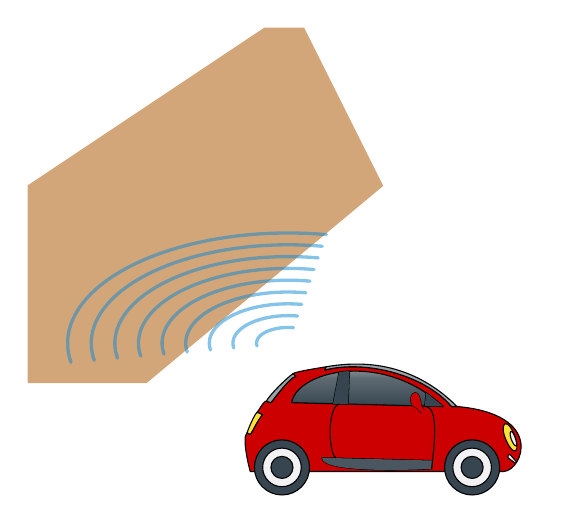
\begin{tikzpicture}[>=latex,line join=round,line cap=round,scale=1,transform shape]
				 \definecolor{bostonuniversityred}{rgb}{0.8,0.0,0.0}
				\definecolor{charcoal}{rgb}{0.21,0.27,0.31} 
				 \definecolor{bananayellow}{rgb}{1.0,0.88,0.21}
				 \definecolor{anti-flashwhite}{rgb}{0.95,0.95,0.96}
				\tikzset{ 
					xeoto/.pic={ 
				\tikzset{xe/.pic={ 
				 \def\N{
					(-2.7,.56)--(-2.5,.56) 
					..controls +(50:1.5) and  +(165:1.5).. (2.1,1.88)--(2.05,2)
					..controls +(-10:.1) and +(130:.1).. (3.25,1.75)--(3.15,1.65) 
					..controls +(-4:.2) and  +(130:.15).. (4.05,.7)--(4.25,.75)
					..controls +(-40:.2) and  +(130:.15).. (4.55,.35)--(4.35,.26)
					 ..controls +(-40:.2) and +(130:.15).. (4.8,-.45)--(4.92,-.4)
					 ..controls +(-40:.25) and +(73:.17).. (4.8,-1.8)--(-4.4,-1.8)
					..controls +(175:.7) and +(-175:3.2)..cycle; 
				 }
				 \fill[bostonuniversityred] \N;
				 \draw \N;
				\def\K{ 
					 (-2.2,.56)--(3.3,.7)
					..controls +(100:1.18) and  +(43:3).. cycle;
				 }
				\fill[bottom color=charcoal,top color=charcoal!20!white,middle  color=charcoal!80!white] \K;
				 \draw \K;
				\def\K1{ 
					(-2.2,.56) 
					..controls  +(43:.2) and +(43:.2).. (-1.58,1.05)--(-1.53,.57)--cycle;
				 }
				\draw \K1; 
				\fill[charcoal] \K1; 
				 \def\K2{
					 (1.2,1.85)
					..controls +(-10:.1) and +(160:.1)..  (1.58,1.8)--(1.8,.65)--(1.25,.65)--cycle;
				} 
				\draw  \K2;
				\fill[charcoal] \K2; 
				 \def\Kt{
					(-2.5,.56) 
					 ..controls +(50:1.5) and +(165:1.5).. (2.1,1.88)--(2.05,2)
					 ..controls +(170:2.2) and +(45:1.5).. (-2.7,.56)--cycle;
				} 
				\fill[charcoal!50]  \Kt;
				 \draw \Kt;
				 \def\Ks{
					 (3.25,1.75)--(3.15,1.65)
					..controls  +(-4:.2) and +(130:.15).. (4.05,.7)--(4.22,.75)
					..controls +(120:.3) and  +(-35:.3).. cycle;
				 }
				\fill[charcoal!50]  \Ks;
				 \draw \Ks;
				\def\D{ 
					(4.55,.35)--(4.35,.26) 
					..controls +(-40:.2) and +(130:.15).. (4.8,-.45)--(4.92,-.4) 
					..controls +(110:.2)  and +(-40:.15)..cycle;
				} 
				 \fill[bananayellow] \D;
				\draw \D; 
				\def\M{ 
					(2.2,-1.3)--(-1.8,-1.4)--(-1.78,-1.7) 
					..controls +(-5:.3) and +(-90:.6)..cycle; 
				 }
				\draw \M; 
				\fill[charcoal!90]  \M;
				\draw (-1.6,.55) 
					..controls +(-170:.5) and +(95:.4).. (-1.78,-1.7) 
					(1.6,.65) 
					..controls +(-30:.5) and +(35:.3)..  (1.7,-1.3);
				\def\G{ 
					(-1.5,.45)--(-1.4,.6) 
					..controls +(85:1)  and +(20:.6).. (-1.25,.5)--(-1.4,.33);
				 }
				 \draw \G;
				 \fill[bostonuniversityred] \G;
				 \def\Dt{
					 (-4.85,-.7)
					..controls +(75:1) and +(65:.8).. (-4.5,-.7) 
					..controls  +(-115:.6) and +(-105:.4).. cycle;
				} 
				\fill[bananayellow] \Dt; 
				 \draw \Dt;
				\def\Dt2{ 
					(-4.85,-.7) 
					..controls +(75:.6) and +(65:.4).. (-4.7,-.7) 
					..controls +(-115:.3) and +(-105:.2)..  cycle;
				 }
				 \fill[anti-flashwhite] \Dt2;
				\draw  \Dt2;
				 \draw[fill=anti-flashwhite] (-4.86,-1.45)--(-4.82,-1.5)--(-4.55,-1.3)
					..controls +(90:.3) and +(45:.2).. cycle; 
					}} 
				\tikzset{banh_xe/.pic={ 
				 \draw[fill=charcoal] (-3.25,-1.65) circle (1);
				\draw[fill=anti-flashwhite]  (-3.25,-1.65) circle (.7);
				\draw[fill=charcoal] (-3.25,-1.65)  circle (.4);
					}} 
				 \path
					 (0,0) pic[scale=1]{xe}
					(0,0) pic[scale=1]{banh_xe} 
					 (6.9,0) pic[scale=1]{banh_xe};
					}} 
				 \def\bc{5}
				\def\ba{2.8} 
				\def\gocM{150} 
				\coordinate (M) at  (0,0);
				\coordinate (C) at  (0:\bc);
				\coordinate (A)  at (\gocM:\ba);
				 \coordinate (B) at (-\gocM:\ba);
				 \pic[scale=0.35,xscale=-1] at (M) [pic type = xeoto];
				\fill[brown!70,draw](-3,0.5)--(0,3)--(-1,5)--(-4,3)--cycle (-3,0.5)--(-4.5,0.5)--(-4.5,3)--(-4,3)--cycle (-4.5,3)--(-1.5,5)--(-1,5)--(-4,3)--cycle; 
				 \foreach \r in {0.4,0.7,1.0,1.3,1.6,1.9,2.2,2.5,2.8}{
					\draw[cyan!70!blue,line  width=1.2pt,opacity=0.5,domain=-10:100,samples=40]
					plot ({-1.2-\r*cos (\x)},{1+\r*sin  (\x)/2});
				} 
			\end{tikzpicture}
	\end{center}
	Một người lái xe đang lùi thẳng về phía một mặt phẳng nghiêng, được cho bởi phương trình là $(E)\colon6x+2y+3z=49$. Xác định được điểm $R(a; b;c)$ trên đoạn $PQ$ trong đó  $P(6;3;1)$ và $Q(6;4;1)$ mà tại đó cảm biến bắt đầu báo động. Tính $a-b+c$ (\textit{làm tròn kết quả đến hàng phần trăm})
	 \shortans{3,05}
	 \loigiai{
		Đường thẳng $PQ$ (dạng tham số)  là
		$\heva{&x=6\\&y=3+t\\&z=1.}$\\ 
		Điểm $R$  trên đoạn $PQ$ khi cảm biến bắt đầu báo động.\\
		Suy ra $R(6;3+t;1)$.\\ 
		Khoảng cách từ $R$  đến $(E)$ là $\mathrm{d}=\dfrac{\left|36+2(3+t)+3-49\right|}{7}=\dfrac{|-4+2t|}{7}$.\\
		Cảm biến bắt  đầu báo động nên $4-2t=\dfrac{21}{10} \Rightarrow t=\dfrac{19}{20}$.\\
		 Suy ra $R\left(6;3+\dfrac{19}{20};1\right)=\left(6;\dfrac{79}{20};1\right)$.
		\\ 
		 Do đó $a-b+c=6-\dfrac{79}{20}+1\approx 3{,}05$.
	} 
\end{bt}

% nguồn: Phan2_Lop_12_Hinh_hoc_Chuong_5
\begin{bt}%[2H5V1-7]%[ma:5750d751]
	Trong hoạt động quay phim và chụp ảnh chuyên nghiệp, tấm hắt sáng là một công cụ không thể thiếu. Một ê-kíp nhận dự án chụp hình cho một căn hộ phục vụ cho mục đích quảng cáo. Tấm hắt sáng được đặt trên một bề mặt gỗ mỏng hình tam giác, mỗi đỉnh của mặt gỗ đặt trên một chiếc cọc lần lượt cao $2$ m, $1$ m và $0{,}5$ m. Cọc cao nhất đặt ở  góc tường, cọc cao $1$ m sẽ đặt ở tường sau nhà, cách tường trái $2$ m, cọc còn lại đặt ở tường bên trái, cách tường sau $1$ m. Để đảm bảo sự chắc chắn, người ta chống một chiếc cọc vuông góc mặt đất và đỡ phía dưới mặt gỗ, cách mỗi bức tường $0{,}5$ m (\textit{chân cọc chống đỡ ở mặt đất}).
	\begin{center}
		\begin{tikzpicture}[line join=round,line cap=round,>=stealth,font=\footnotesize,scale=0.8]
				\clip (-7,-1) rectangle  (7,7);
				\def\g{-150}  \def\d{2cm}
				 \path
					 (-3,0.3) coordinate (A)
					(-2,1.8)  coordinate (B)
					 (-0.5,1) coordinate (C);
				\draw (1,2.5)--(-2,2.5)--++(\g:\d)--++(-90:\d)--++(180+\g:\d)--++(0:3) 
					(-2,0.5)--(-2,2.5); 
				\draw[fill=gray!30]  (A)--(B)--(C)--(A);
				\draw  [line width=1.5pt]
					 (A)--++(-90:0.35)
					(B)--++(-90:1.3) 
					 (C)--++(-90:0.5)
					 (-1.7,0.9)--++(-90:0.6);
			\draw[->] (-1.8,1.4) arc[start angle=-30,end angle=90,radius=1.5cm]node[left]{tấm hắt sáng};
		\end{tikzpicture}
	\end{center}
	Hỏi chiếc cọc chống đỡ  này có chiều dài bao nhiêu mét?
	\shortans{1} 
	 \loigiai{
		Gắn hệ tọa độ  $Oxyz$ vào phía góc tường, điểm $0(0;0;0)$ trùng với chân góc tường, trục cao $Oz$ trùng với cọc cao nhất và hai trục $Ox$, $Oy$ lần lượt là hai đường chân tường. Mỗi đơn vị ứng với $1$ mét thực tế.
		Đỉnh của các cọc có chiều cao giảm dần lần lượt là các điểm $A$, $C$, $B$. Chiếc cọc chống đặt tại điểm $E$ và điểm tiếp xúc giữa mặt gỗ và  cọc chống là điểm $H$.
		\begin{center}
			\begin{tikzpicture}[line join=round,line cap=round,>=stealth,font=\footnotesize,scale=0.8]
					 \def\g{-135}
					 \path
						(0,0) coordinate (O) 
						++(90:4) coordinate  (A)
						(0:4) coordinate (M)++(90:3) coordinate  (C)
						(\g:3) coordinate (N)++(90:2)  coordinate (B)
						($(M)!0.5!(O)+(O)!0.5!(N)-(O)$) coordinate (E)++(90:3.5) coordinate (H) 
						(intersection of B--C and E--H) coordinate (I); 
					\draw [->] (O)--(0:5)  node[above]{$x$};
					 \draw[->] (O)--(\g:4) node[right]{$y$};
					\draw[->]  (O)--(90:5) node[right]{$z$};
					 \draw (A)--(B)--(C)--(A);
					\draw [line width=1.5pt] (O)--(A) 
						 (M)--(C)
						 (N)--(B)
						(E)--(I); 
					\draw  [line width=1.5pt,dashed] (I)--(H);
					\draw  [dashed]($(M)!0.5!(O)$)--(E)--($(O)!0.5!(N)$);
					\foreach \i/\g in {O/180,A/180,C/30,B/160,E/-90,H/90}{\draw (\i) circle (1pt) 
						 ($(\i)+(\g:3mm)$) node[scale=1]{$\i$};}
				\end{tikzpicture}
		\end{center}
		Theo đề bài, ta được tọa độ các điểm: $A\left(  0;0;2\right) $; $C\left( 2;0;1\right) $; $B\left( 0;1;\dfrac{1}{2}\right) $; $E\left( \dfrac{1}{2};\dfrac{1}{2};0\right) $.\\
		Khi đó chiều dài cọc chống chính là độ dài đoạn thẳng $HE$ và $H$ là điểm thỏa mãn nằm trên mp$ (ABC)$ sao cho $EH$ cùng phương với $OA$.\\ 
		 Ta có: $\overrightarrow{AB}=\left( 0;1;-\dfrac{3}{2}\right)$ và $\overrightarrow{AC}=(2;0;-1)$.\\
		Mặt phẳng $(ABC)$ nhận  $\overrightarrow{n}=\left[\overrightarrow{AB}; \overrightarrow{AC}\right]$ là vectơ pháp tuyến.\\
		Có $\overrightarrow{n}=\left[\overrightarrow{AB}; \overrightarrow{AC}\right]=(-1;-3;-2)$.\\ 
		Khi đó mặt  phẳng $(ABC)$ có phương trình
		\begin{align*}
			&-1(x-0)-3(y-0)-2(z-2)=0\\ 
			&\Leftrightarrow x+3y+2z-4=0. 
		\end{align*}
		Gọi điểm $H  (x;y;z) \Rightarrow \overrightarrow{EH}=\left( x-\dfrac{1}{2};y-\dfrac{1}{2};z\right) $.\\
		Có $\overrightarrow{OA}=(0;0;2)$.\\ 
		Mà $\overrightarrow{EH}$  cùng phương với $\overrightarrow{OA} \Rightarrow \overrightarrow{EH}=k\overrightarrow{OA}$.
		\begin{align*}
			\overrightarrow{EH}=\left(0,0,2k \right) \Rightarrow  \heva{&x-\dfrac{1}{2}=0\\&y-\dfrac{1}{2}=0\\&z=2k}\Leftrightarrow\heva{&x=\dfrac{1}{2}\\&y=\dfrac{1}{2}\\&z=2k}\Rightarrow H\left(\dfrac{1}{2}; \dfrac{1}{2};2k \right).
		\end{align*}
		Lại có $H\in\left(ABC \right) \Rightarrow \dfrac{1}{2}+3\cdot \dfrac{1}{2}+2\cdot  2k-4=0 \Rightarrow k=\dfrac{1}{2}\Rightarrow H\left(\dfrac{1}{2}; \dfrac{1}{2};1 \right)$.\\
		Khi đó $\overrightarrow{EH}=  \left(0;0;1 \right) \Rightarrow EH=1 $.\\
		Như  vậy chiều dài cọc chống đỡ này là $1$ mét.
	 }
\end{bt}

% nguồn: Phan2_Lop_12_Hinh_hoc_Chuong_5
\begin{bt}%[2H5V1-7]%[ma:216d1c3b]
	Sân quần vợt được mô hình hóa lý tưởng,  có chiều dài $24$ m và chiều rộng $10$ m. Các ô giao bóng dài $6$ m và rộng $5$ m. Lưới cao liên tục $1$ m. Mọi cú đánh đều bay theo đường thẳng.
	\begin{center}
		\begin{tikzpicture}[>=stealth,line join=round,line cap=round,font=\footnotesize,scale=1]
				\coordinate (O) at  (0,0);
				 \coordinate (A) at (2.5,0);
				\coordinate (B)  at (5,0);
				\coordinate (C)  at (7.5,0);
				\coordinate (E)  at (10,0);
				 \coordinate (D) at (-2,-3);
				\coordinate  (S) at (0.5,-3);
				\coordinate (F)  at (3,-3);
				 \coordinate (I) at (5.5,-3);
				\coordinate (G)  at (8,-3);
				\coordinate (T)  at ($(A)!0.5!(S)$);
				 \coordinate (H) at ($(E)!0.5!(F)$);
				 \coordinate (K) at ($(O)!0.55!(D)$);
				\coordinate (Y) at  ($(D)!1/3!(S)$);
				\coordinate (P) at ($(E)!0.3!(G)$); 
				\fill[green!30!white](-0.5,0.5)--(-3,-3.5)--(8.5,-3.5)--(11,0.5)--cycle; 
				\draw[->,line width=2pt](O)--(10.5,0)  node[below]{$y$};
				 \draw[->,line width=2pt](O)--(0,2) node[left]{$z$};
				\draw[->,line width=2pt](O)--($(O)!1.1!(D)$) node[right]{$x$}; 
				\fill[orange!50!pink,draw](O)--(D)--(G)--(E)--cycle; 
				\draw[white,line  width=2pt](A)--(S)
					(T)--($(C)!0.5!(I)$) 
					(I)--(C); 
				\draw[line width=2pt](K)--($(K)+(0,0.4)$) 
					(P)--($(P)+(0,1)$) 
					($(P)+(0,1.1)$)--($(P)+(0,1.2)$); 
				\fill[yellow,draw]($(K)+(0,0.4)$) circle (2 pt) 
					($(P)+(0,1.3)$) circle (2pt); 
				\fill[white,draw]($(P)+(0,1)$) circle  (2 pt);
				\draw[dashed,cyan,line width=2pt]($(K)+(0.1,0.4)$)--(T); 
				\draw[cyan,line width=2pt]($(P)+(-0.1,1.3)$)--(T); 
				 \draw[red,line width=2pt](B)--($(B)+(0,0.5)$)
					 (F)--($(F)+(0,0.5)$);
				\fill[white,pattern=grid](B)--($(B)+(0,0.5)$)--($(F)+(0,0.5)$)--(F)--cycle; 
				\draw (K)  node[left]{$K$};
				\draw (P)  node[right]{$P$};
				\foreach \i/\g  in {S/-90,Y/-90}{\draw[fill=white](\i) circle (2pt)
					($(\i)+(\g:3mm)$)  node[scale=1]{$\i$};}
				\foreach \i/\g in  {T/90}{\draw[fill=yellow](\i) circle (2pt)
					 ($(\i)+(\g:3mm)$) node[scale=1]{$\i$};}
			\end{tikzpicture}
	\end{center}
	Một vận động viên đứng ở vạch cuối sân tại điểm $P(3;24;0)$ và cố gắng đánh quả bóng với vận tốc $144$ km/h ở độ cao $3{,}10$ m sao cho bóng rơi đúng vào điểm $T(5;6;0)$ của ô giao bóng. Sau khi chạm  đất, bóng phản xạ theo góc $\alpha$ (giữ nguyên vận tốc, không đổi hướng ngang). Tại vị trí $K$ trên vạch cuối sân bên kia đối thủ sẽ đánh trả, hãy tính thời gian đối thủ có để phản ứng là bao nhiêu giây? (\textit{làm tròn kết quả đến hàng phần trăm})
	\shortans{0,15} 
	 \loigiai{
		Quỹ đạo từ $A$ đến $T$ là đường thẳng $AT\colon \heva{&x=3+2 t\\&y=24-18t\\&z=3{,}10-3{,}1t}$, $(0 \le  t \le 1)$ và hướng $\overrightarrow{v}=(2;-18;-3,1)$.\\
		Sau nảy bóng phản xạ giữ nguyên vận  tốc, không đổi hướng ngang.\\
		Hướng mới $\overrightarrow{v'}=(2;-18;  3{,}1)$.\\
		Vậy phương trình mới  của quả bóng là $\heva{&x=5+2s\\&y=6-18s\\&z=3{,}1}$, $(s \in \mathbb{R})$.\\
		Điểm $K$ trên vạch cuối sân bên kia  thuộc mặt phẳng $y=0$.\\
		Suy ra  $6-18 s=0 \Rightarrow s=\dfrac{1}{3} \Rightarrow K\left(\dfrac{17}{3};0;\dfrac{31}{30}\right)$.\\
		Quãng đường  $TK=\sqrt{\left(\dfrac{17}{3}-5\right)^{2}+6^{2}+\left(\dfrac{31}{30}\right)^{2}}=\dfrac{7 \sqrt{689}}{30}$.\\
		Đổi vận tốc $144$  km/h $=40$ m/s.\\
		Thời gian đối thủ có để phản  ứng là $t=\dfrac{TK}{40} \approx 0{,}15$ (s).
	 }
\end{bt}

% nguồn: Phan2_Lop_12_Hinh_hoc_Chuong_5
\begin{bt}%[2H5V1-7]%[ma:27467620]
	Trong không gian $Oxyz$, một cabin cáp treo xuất phát từ điểm $A(10; 3; 0)$ và chuyển động đều theo đường cáp có vectơ chỉ phương là $\vec{u}=(2;-2; 1)$ với tốc độ là $4{,}5$ m/s. Sau thời gian $180$  giây, Cabin dừng ở điểm $B$. Tìm tung độ điểm $B$.
	\shortans{-537} 
	 \loigiai{
		Phương  trình tham số của đường thẳng đi qua điểm $A$ với vectơ chỉ phương $\vec{u}$ là
		$\heva{&x=10+2t \\&y=3-2t \\&z=0+1  t.}$\\
		Với $t$ là tham số đại diện  cho khoảng dịch chuyển trên đường thẳng theo vectơ chỉ phương $\vec{u}$.\\
		Ta có $|\vec{u}|  = \sqrt{2^2 + (-2)^2 + 1^2} = \sqrt{4 + 4 + 1} = \sqrt{9} = 3.$\\
		Quãng đường cabin di chuyển sau thời gian  $t = 180$ giây với tốc độ $v = 4{,}5$ m/s là\\
		$s = v \cdot t = 4{,}5 \cdot 180 = 810$  m.\\
		Giá trị tham số $t$  ứng với quãng đường $s$:
		$s  = |\vec{u}| \cdot t \Rightarrow t = \dfrac{s}{|\vec{u}|} = \dfrac{810}{3} = 270$.\\
		Tọa độ điểm $B$ là $\heva{&x_B = 10 + 2 \cdot 270 =  550 \\&y_B = 3 - 2 \cdot 270 = -537 \\&z_B = 0 + 1 \cdot 270 = 270.}$\\
		Vậy tung độ của điểm $B$  là $-537$.
	} 
\end{bt}

% nguồn: Phan2_Lop_12_Hinh_hoc_Chuong_5
\begin{bt}%[2H5V1-7]%[ma:25811aa1]
	Một hộ gia đình muốn làm chiếc lều. Đáy nằm trên nền đất phẳng, các cột vuông góc với đáy có chiều cao $AA'=DD'=1{,}5$m, $BB'=CC'=2$m, đáy là hình chữ nhật có $AB=2$m, $AD=1{,}5$m (tham khảo hình vẽ minh hoạ). Góc tạo  bởi mái nhà và nền nhà là bao nhiêu độ (làm tròn đến hàng đơn vị)
	\begin{center}
		\begin{tikzpicture}[scale=0.7,>=stealth,x=1cm,y=1cm,font=\footnotesize,line join=round,line cap=round]
				 \path
					 (0,0) coordinate (D)
					(-2,-2) coordinate (A) 
					 (3,-2) coordinate (B)
					(5,0)  coordinate (C)
					 (-2,2) coordinate (A')
					(3,4) coordinate (B') 
					(5,6)  coordinate (C')
					(0,4) coordinate  (D');
				\draw (A)--(B)--(C) 
					 (A')--(B')--(C')--(D')--(A')
					 (B)--(B')
					(C)--(C') 
					 (A)--(A');
				 \draw[dashed] (A)--(D)--(D');
				\foreach \x/\g in {A/180,B/0,C/0,D/180,A'/180,B'/0,C'/0,D'/180} 
				\fill (\x) circle  (0.8pt)
					($(\x)+(\g:3mm)$) node{\x}; 
				 \draw[dashed,fill=pink,opacity=0.7] (D)--(A)--(B)--(C)--(D)-- cycle;
			\end{tikzpicture}
	\end{center}
	 \shortans{14}
	\loigiai{ 
		\begin{center}
			\begin{tikzpicture}[scale=0.7,>=stealth,x=1cm,y=1cm,font=\footnotesize,line join=round,line cap=round]
					 \draw[->](5,0)--(6,0);
					\draw[->](-2,-2)--(-3,-3); 
					\draw[->](0,4)--(0,5); 
					\draw (6,0)  node[above]{$y$}
						(-3,-3) node[left]{$x$} 
						(0,5)  node[left]{$z$};
					 \path
						 (0,0) coordinate (D)
						(-2,-2) coordinate  (A)
						(3,-2) coordinate (B) 
						(5,0) coordinate  (C)
						(-2,2) coordinate  (A')
						(3,4)  coordinate (B')
						(5,6) coordinate  (C')
						(0,4) coordinate  (D');
					 \draw (A)--(B)--(C)
						(A')--(B')--(C')--(D')--(A') 
						(B)--(B') 
						(C)--(C') 
						 (A)--(A');
					\draw[dashed]  (A)--(D)--(D');
					\foreach \x/\g  in {A/180,B/0,C/40,D/180,A'/180,B'/0,C'/0,D'/180}
					\fill  (\x) circle (0.8pt)
						($(\x)+(\g:3mm)$) node{\x}; 
					\draw[dashed,fill=pink,opacity=0.7] (D)--(A)--(B)--(C)--(D)-- cycle; 
				\end{tikzpicture}
		\end{center}
		Chọn hệ trục $Oxyz$ với gốc tọa độ $D(0;0;0)$. Khi đó ta có $D'(0; 0; 1{,}5), A'(1{,}5; 0; 1{,}5), B'(1{,}5; 2; 2)$.\\ 
		 $$
		\begin{aligned}
			& \overrightarrow{D'A'}=(1{,}5; 0; 0)=1{,}5(1;  0; 0)\,\, \overrightarrow{D'B'}=(1{,}5; 2; 0{,}5)=0{,}5(3; 4; 1) . \\& \left[\overrightarrow{D'A'}, \overrightarrow{D' B'}\right]=(0;-1;-4)=-(0; 1; 4) \text {là véctơ pháp tuyến của }\left(A' B'C'D'\right).
		\end{aligned}
		$$ 
		Mặt $(A B C D)$ có vecto pháp tuyến là $\vec{k}=(0; 0;  1)$.\\
		Ta có$ 
		\cos \left((A B C D),\left(A' B'C'D'\right)\right)=\dfrac{|4|}{\sqrt{17}}=\dfrac{4}{\sqrt{17}}  \Rightarrow\left((A B C D),\left(A'B'C'D'\right)\right) \approx 14^{\circ}. $
	 }
\end{bt}

% nguồn: Phan2_Lop_12_Hinh_hoc_Chuong_5
\begin{bt}%[2H5V1-7]%[ma:5a58f70f]
	Một buổi biểu diễn sân khấu diễn ra trên một sân khấu nghiêng về  phía khán giả.
	\begin{center}
		\begin{tikzpicture}[line join=round,line cap=round,>=stealth,font=\footnotesize,scale=0.7]
				 \def\d{1}
				 \path
					 (0,0) coordinate (O)
					(-150:2*\d) coordinate  (A)
					(0:7*\d) coordinate  (C)
					 ($(A)+(C)-(O)$) coordinate (D)
					 (90:\d) coordinate (F)
					(C)++(90:\d)  coordinate (E)
					++(90:2.5*\d) coordinate  (B);
				\draw (D)--(A)--(F)--(E)--(D)--(C) node[midway,below right]{$8$}--(E)  node[midway,right]{$2$};
				\draw [dashed] (E)--(B) 
					 (A)--(O)--(C)
					(O)--(F); 
				 \draw [->] (O)--(90:\d/2) node[left]{$z$};
				\draw  [->] (O)--(0:\d) node[below]{$y$};
				\draw [->] (O)--(-150:\d/2)  node[below right]{$x$};
				\foreach \i/\g in {A/180,O/-45,D/-30,E/0,B/0}{\draw (\i) circle (1pt) 
					 ($(\i)+(\g:3mm)$) node[scale=1]{$\i$};}
			\end{tikzpicture}
	\end{center}
	Cuối buổi biểu diễn, nữ diễn viên chính rời sân khấu trong một chiếc ghế treo trên dây, di chuyển từ điểm $A(8;0;0)$ đến điểm $B(0;20;10)$. Sau khi đi được $\dfrac{3}{4}$ quãng đường, cô ấy dừng lại để  thực hiện động tác cuối. Hãy tính khoảng cách của cô ấy đến mặt phẳng sân khấu tại thời điểm đó (\textit{làm tròn kết quả đến hàng phần trăm}).
	\shortans{5,82} 
	 \loigiai{
		Gắn hệ trục tọa  độ $Oxyz$ như hình vẽ, ta có $A(8;0;0)$, $D(8;20;0)$ và $E (0;20;2)$.\\
		Xét mặt phẳng sân  khấu $\left(ADE\right)$ có vectơ pháp tuyến $\overrightarrow{n}=(40;0;160)$ rút gọn được $\overrightarrow{n}=(1;0;4)$.\\
		Phương trình mặt phẳng  $\left(ADE \right)$ qua điểm $A(8;0;0)$ nên ta có
		\begin{align*}
			1(x-8)+0(y- 0)+4(z-0)=0 \\ 
			\Leftrightarrow  x+4z-8=0
		\end{align*}
		Di chuyển treo  dây từ $A(8;0;0)$ đến $B(0;20;10)$ và dừng ở $\dfrac{3}{4}$ quãng đường.\\
		Do đó điểm dừng  là điểm $C$ thỏa mãn: $\overrightarrow{AC}=\dfrac{3}{4} \overrightarrow{AB} \Rightarrow C(2;15;7{,}5)$.\\
		Khoảng cách  vuông góc của diễn viên đến mặt phẳng sân khấu là
		\begin{align*}
			d(C,E)=\dfrac{2+4\cdot7{,}5-8}{\sqrt{1+4^2}}=\dfrac{24}{\sqrt{17}} \approx 5{,}82. 
		\end{align*}
	} 
\end{bt}

% nguồn: Phan2_Lop_12_Hinh_hoc_Chuong_5
\begin{bt}%[2H5V1-7]%[ma:a35bcfef]
	Hình ảnh bên minh hoạ một cánh cửa hình chữ nhật có chiều rộng $1$ m và chiều cao $2$ m khi đang mở. Chọn hệ toạ độ như hình vẽ, biết cánh  cửa tạo với bức tường một góc $30^{\circ}$, bờ tường vuông góc với mặt sàn. Bỏ qua bề dày của cánh cửa thì phương trình mặt phẳng chứa cánh cửa là $x + by + cz + d = 0$. Tính giá trị $9b^2 + 3c^2 + d$.
	\begin{center}
		\begin{tikzpicture}[line join=round,line cap=round,>=stealth,scale=0.8]
				 \def\a{4} \def\b{0.5}
				\path (0,0) coordinate (O) 
					(20:0.1*\a) coordinate  (I)
					($(I)+(0,1.53*\a)$) coordinate (J) 
					(-25:0.5*\a)  coordinate (x)
					(20:\a) coordinate  (y)
					 (90:1.63*\a) coordinate (z)
					(90:1.45*\a) coordinate (A) 
					(220:.6*\a) coordinate  (B)
					($(B)+(-0.1,0.05)$)  coordinate (b)
					 ($(y)!2.2!(O)$) coordinate (t)
					 ($(O)!.5!(y)$) coordinate (L)
					($(O)!.6!(y)$)  coordinate (w)
					 ($(A)+(B)-(O)$) coordinate (C)
					($(b)+(C)-(B)$) coordinate  (c)
					($(c)+(A)-(C)$) coordinate  (q)
					 ($(y)+(B)-(O)$) coordinate (v)
					(intersection of B--v and O--x) coordinate (N) 
					($(O)+(B)-(N)$) coordinate (M) 
					 ($(A)+(M)-(O)$) coordinate (D)
					(intersection of c--q and A--D)  coordinate (a)
					($(O)!1.125!(M)$) coordinate (H) 
					($(H)+(0,0.1*\a)$)  coordinate (h)
					 ($(t)+(h)-(H)$) coordinate (T)
					($(I)+(0,0.1*\a)$) coordinate (i) 
					 ($(L)+(0,0.1*\a)$) coordinate (l)
					 ($(H)+(J)-(I)$) coordinate (K)
					($(A)!0.5!(O)$)  coordinate (E)
					 ($(A)!0.5!(C)$) coordinate (F)
					($(C)!0.45!(B)$) coordinate (r) 
					($(r)+(0.2,0)$) coordinate (X) 
					($(A)!0.5!(C)$)  coordinate (F)
					 ($(O)!0.5!(B)$) coordinate (p)
					($(H)!0.5!(M)$) coordinate (m); 
				\draw[->] (O)--(z)  node[above]{$z$};
				\fill  [orange!30](O)--(I)--(J)--(K)--(H)--(M)--(D)--(A)--cycle;
				\draw (I)--(J)--(K)--(H) 
					 (A)--(J)
					(D)--(K) 
					(t)--(M); 
				 \draw (O)--(A)--(D)--(M);
				 \draw (O)--(A)--(C)--(B)--cycle;
				\draw  (t)--(T)--(h)--(H)--cycle;
				 \fill [orange!30](t)--(T)--(h)--(H)--cycle;
				\draw (I)--(L)--(l)--(i)--cycle; 
				\fill [orange!30](I)--(L)--(l)--(i)--cycle; 
				 \draw (B)--(b)--(c)--(C)--cycle;
				\fill  [orange!10](B)--(b)--(c)--(C)--cycle;
				\draw (C)--(c)--(a)--(A)--cycle; 
				\fill  [orange!10](C)--(c)--(a)--(A)--cycle;
				\fill [orange!30](A)--(O)--(B)--(C)--cycle; 
				\draw[->] (O)--(w) node[above  right]{$y$};
				\draw[->] (O)--(x)  node[below right]{$x$};
				\draw [fill=orange!10,rotate=-5] (X) ellipse (4pt and 5pt); 
				\draw (r)+(180:4 mm) node[rotate=90]  {$2\text{ m}$};
				\draw (p)+(0:4  mm) node[rotate=45] {$1\text{ m}$};
				\draw[->] 
					(m)..  controls (-2.7,-1.6) and (-2.2,-1.6).. (b);
				\draw (-2.7,-1.7) node  {$30^\circ$};
			\end{tikzpicture}
	\end{center}
	 \shortans{3}
	 \loigiai{
		\begin{tikzpicture}[line join=round,line cap=round,>=stealth]
				 \def\a{4}
				 \path (0,0) coordinate (O)
					(-25:\a) coordinate  (x)
					(20:\a) coordinate  (y)
					(90:1.3*\a) coordinate  (z)
					(90:1.1*\a) coordinate  (A)
					(230:.6*\a) coordinate  (B)
					 ($(y)!2!(O)$) coordinate (t)
					($(A)+(B)-(O)$) coordinate  (C)
					($(y)+(B)-(O)$) coordinate (v) 
					(intersection of B--v and  O--x) coordinate (N)
					 ($(O)+(B)-(N)$) coordinate (M)
					($(A)!0.5!(O)$)  coordinate (E)
					($(A)!0.5!(C)$) coordinate  (F);
				\draw (A)--(O)--(B)--(C)--cycle; 
				 \fill [orange!30](A)--(O)--(B)--(C)--cycle;
				\draw[dashed] (M)--(B)--(N); 
				\draw[->] (t)--(y) node[above right]{$y$}; 
				 \draw[->] (O)--(x) node[below right]{$x$};
				\draw[->] (O)--(z) node[above]{$z$}; 
				\foreach \x/\g  in {B/-85,O/50,M/90,N/20}
				\fill  (\x) circle (1pt)
					($(\g:3mm)+(\x)$)  node {$\x$};
				 \draw (A) circle (1pt) node [right]{$A (0; 0; 2)$};
				\draw (E) circle (0pt)  node [right]{$2\text{ m}$};
				\draw (F)  circle (0pt) node [above left]{$1\text{ m}$};
				\begin{scope}
					\clip (M)--(O)--(B); 
					\draw  (O) circle (4.5mm);
				\end{scope}
				 \draw (O)+(218:9 mm) node[font=\footnotesize] {$30^\circ$};
			\end{tikzpicture}
		\hspace{2cm} 
		\begin{tikzpicture}[line join=round,line cap=round,>=stealth]
				 \def\a{4}
				 \path (0,0) coordinate (M)
					 (5,0) coordinate (O)
					(0,3) coordinate  (B);
				 \draw (M)--(O)--(B)--cycle;
				\begin{scope}
					\clip (M)--(O)--(B); 
					 \draw (O) circle (4.5mm);
				\end{scope}
				\draw (O)+(167:8  mm) node[font=\footnotesize] {$30^\circ$};
				 \foreach \x/\g in {B/90,O/0,M/200}
				 \fill (\x) circle (1pt)
					($(\g:3mm)+(\x)$)  node {$\x$};
			\end{tikzpicture}
		\noindent 
		Giả sử $(H) \colon x + by  + cz + d = 0$.\\
		Vì ta đã có dạng của phương trình mặt phẳng chứa cánh  cửa (chứa 3 ẩn $b$, $c$, $d$) nên để viết được phương trình mặt phẳng $(H)$, ta cần đi tìm được 3 điểm thuộc mặt phẳng đó.\\
		Ta  vẽ lại hình như và kí hiệu các điểm như hình sau\\
		Với $A$, $B$, $O$ là các điểm thuộc  mặt phẳng $(H)$. Kẻ
		$\heva{ 
		 &BM \perp Oy\\
		 &BN \perp Ox
		.}$\\ 
		Dựa vào hình vẽ, ta thấy mặt phẳng  cần tìm đi qua các điểm $A(0;0;2)$, $O(0;0;0)$, $B(BM;-OM;0)$.\\
		 Trong tam giác $OBM$ vuông tại $M$, ta có\\
		$\cos{\widehat{BOM}}  = \dfrac{OM}{OB} \Rightarrow OM = OB \cdot \cos{\widehat{BOM}} = 1 \cdot \cos{30^{\circ}} = \dfrac{\sqrt{3}}{2}$.\\
		$\sin{\widehat{BOM}} = \dfrac{BM}{OM} \Rightarrow BM =  OB\cdot \sin{\widehat{BOM}} = 1 \cdot \sin{30^{\circ}} = \dfrac{1}{2}$.\\
		 Suy ra $B\left(\dfrac{1}{2};-\dfrac{\sqrt{3}}{2};0\right)$.\\
		Vì $A(0;0;2)$, $O(0;0;0)$, $B\left(\dfrac{1}{2};-\dfrac{\sqrt{3}}{2};0\right)$ đều thuộc  mặt phẳng $(H)$ nên ta có hệ phương trình
		$$\heva{ 
		 &2c + d = 0\\
		&d  = 0\\
		&\dfrac{1}{2} - \dfrac{\sqrt{3}}{2}b + d  = 0
		 } \Leftrightarrow
		 \heva{
		 &c = 0\\
		&d  = 0\\
		&b =  \dfrac{1}{\sqrt{3}}.
		 }$$\\
		Vậy $9b^2 + 3c^2 + d = 9 \cdot \left(\dfrac{1}{\sqrt{3}}\right)^2 =  3$.
	} 
\end{bt}

% nguồn: Phan2_Lop_12_Hinh_hoc_Chuong_5
\begin{bt}%[2H5V1-7]%[ma:d08ace7d]
	Chọn hệ trục tọa độ $Oxyz$ sao cho $O$ nằm trên  mặt nước, mặt phẳng $(Oxy)$ là mặt nước, trục $Oz$ hướng lên trên (đơn vị độ dài trên các trục tọa độ là mét), một con chim bói cá đang ở vị trí (có hoành độ, tung độ và cao độ là các số thực dương) cách mặt nước $2m$, cách mặt phẳng $(Oxz)$, $(Oyz)$ lần lượt là $3\mathrm{m}$ và $1\mathrm{m}$ phóng thẳng xuống vị trí con cá, biết con cá ở vị trí (có hoành độ và tung độ là các số thực dương) cách mặt nước $50\mathrm{cm}$, cách mặt phẳng $(Oxz)$, $(Oyz)$ lần lượt là $1\mathrm{m}$ và $1{,}5\mathrm{m}$. Tọa độ điểm $B$ lúc chim bói cá vừa tiếp xúc với mặt nước là $(a;b;c)$. Tính $T=4a+3b-25c$.
	\begin{center}
		\begin{tikzpicture}[>=stealth,line cap=round,line join=round]
				\path 
					(0,0)  coordinate (O) node [left]{$O$}
					(5,0)  coordinate (Y)
					(0,5) coordinate  (Z)
					 (-120:5) coordinate (X)
					(3.5,3) coordinate (C) 
					(1,-1) coordinate (B) 
					($(C)!1.2!(B)$) coordinate (A) 
					 ($(X)+(Y)-(O)$) coordinate (M);
				\fill[blue!3]  (O)--(Y)--(M)--(X);
				\draw[->] (O)--(Y) node  [above] {$y$};
				 \draw [->] (O)--(Z) node[left] {$z$};
				\draw[->] (O)--(X) node [left] {$x$}; 
				\fill (3.5,3) circle (1.5pt) node [above] {$C$}; 
				\fill (1,-1) circle (1.5pt) node  [left] {$B$};
				\fill (A) circle (1.5pt)  node [left] {$A$};
				 \draw (C)--(B);
				\draw[dashed] (B)--(A); 
			\end{tikzpicture}
	\end{center}
	\shortans{9,8} 
	\loigiai{ 
		Dựa vào đề bài ta có tọa độ các điểm  $C(1;3;2)$, $A\left(\dfrac{3}{2};1;-\dfrac{1}{2}\right)$, khi đó $\overrightarrow{AC}=\left(-\dfrac{1}{2};2;\dfrac{5}{2}\right)$.\\
		Phương  trình đường thẳng $AC\colon \heva{&x=1-\dfrac{1}{2}t\\&y=3+2t\\&z=2+\dfrac{5}{2}t.}$\\
		Gọi  $B\left(1-\dfrac{1}{2}t; 3+2t; 2-\dfrac{5}{2}t\right)\in AC$.\\
		Ta lại có $B\in (Oxy)$ nên  $2+\dfrac{5}{2}t=0\Leftrightarrow t=-\dfrac{4}{5}$.\\
		Suy  ra $B\left(\dfrac{7}{5};\dfrac{7}{5};0 \right)$.\\
		Vậy  $T=4a+3b-25c=4\cdot\dfrac{7}{5}+3\cdot\dfrac{7}{5}-25\cdot0=\dfrac{49}{5}=9{,}8$.
	} 
\end{bt}

% nguồn: Phan2_Lop_12_Hinh_hoc_Chuong_5
\begin{bt}%[2H5V1-7]%[ma:e748f7e3]
	\immini{Do có ánh kim loại và màu vàng óng, pyrit($FeS_2$) còn được gọi là \textit{vàng găm}. Thường gặp dưới dạng lập phương hoặc bát diện hoàn hảo, đôi khi nhiều tinh thể dính liền nhau. Thỉnh thoảng cũng thấy các khối lập phương pyrit bị mất một góc, tạo thành một hình chóp tam giác đều.  Xét một khối lập phương pyrit cạnh $3$ cm, bị mất một góc dưới dạng hình chóp tam giác đều có các cạnh bên dài $1$ cm. Phương trình của mặt phẳng vỡ có dạng $ax+by+cz+2=0$. Tìm $a+b+c$.}{
	\begin{tikzpicture}[line join=round,line cap=round,>=stealth,font=\footnotesize,scale=0.8]
			 \def\d{4} \def\r{2} \def\h{4} \def\g{-140}
			 \path
				(0,0)  coordinate (O)++(90:\h) coordinate (D) node[above left]{$3$}
				 (0:\d) coordinate (M) node[below]{$3$} ++(90:\h) coordinate (E)++(\g:0.6*\r) coordinate (B)
				(\g:\r)  coordinate (P) node[below right]{$3$}++(90:\h) coordinate (F)++(0:2/3*\d) coordinate (A)
				($(M)+(P)-(O)$)  coordinate (N)++(90:2/3*\h) coordinate (C);
			\draw  (M)--(N)--(P)
				(A)--(B)--(C)--(A)--(F)--(D)--(E)--(B) 
				(C)--(N) 
				 (M)--(E)
				 (P)--(F);
			\draw  [dashed](P)--(O)--(M)
				(O)--(D); 
			\draw[->] (D)--($(D)+(90:1)$) node[right]{$z$}; 
			\draw[->] (M)--($(M)+(0:1)$) node[above]{$y$}; 
			\draw[->] (P)--($(P)+(\g:1)$)  node[left]{$x$};
			\foreach  \i/\g in {O/-45,A/90,B/90,C/-150}{\draw (\i) circle (1pt)
				($(\i)+(\g:3mm)$) node[scale=1]{$\i$};} 
		\end{tikzpicture}
	} 
	 \shortans{-3}
	\loigiai{ 
		\begin{center}
			\begin{tikzpicture}[line join=round,line cap=round,>=stealth,font=\footnotesize,scale=0.8]
					\def\d{4}  \def\r{2} \def\h{4} \def\g{-140}
					\path 
						(0,0) coordinate (O)++(90:\h)  coordinate (D) node[above left]{$3$}
						(0:\d) coordinate (M) node[below]{$3$}  ++(90:\h) coordinate (E)++(\g:0.6*\r) coordinate (B)
						(\g:\r)  coordinate (P) node[below right]{$3$}++(90:\h) coordinate (F)++(0:2/3*\d) coordinate (A)
						($(M)+(P)-(O)$) coordinate (N)++(90:2/3*\h)  coordinate (C);
					 \draw (M)--(N)--(P)
						 (A)--(B)--(C)--(A)--(F)--(D)--(E)--(B)
						 (C)--(N)
						(M)--(E) 
						(P)--(F); 
					\draw  [dashed](P)--(O)--(M)
						 (O)--(D);
					 \draw[->] (D)--($(D)+(90:1)$) node[right]{$z$};
					 \draw[->] (M)--($(M)+(0:1)$) node[above]{$y$};
					 \draw[->] (P)--($(P)+(\g:1)$) node[left]{$x$};
					\foreach \i/\g in  {O/-45,A/90,B/90,C/-150}{\draw (\i) circle (1pt)
						($(\i)+(\g:3mm)$)  node[scale=1]{$\i$};}
				\end{tikzpicture}
		\end{center}
		Ta có $A(3;2;3)$, $B(2;3;3)$,  $C(3;3;2)$.\\
		$\overrightarrow{AB}=(2-3;3-2; 3 -  3)=(-1;1; 0)$.\\
		$\overrightarrow{AC}=(3-3; 3-2; 2 - 3)=(0;1;  -1)$.\\
		vectơ pháp tuyến của mặt phẳng $\left( ABC\right) $ là  $\overrightarrow{n}=\left[\overrightarrow{AB}, \overrightarrow{AC}\right]=(-1;-1;-1)$.\\
		Phương trình mặt phẳng $\left( ABC\right) $ đi qua điểm điểm $A(3;2;3)$ nên  có dạng
		\begin{align*}
			 &-1(x-3)-1(y-2)-1(z-3)=0\\
			&\Leftrightarrow -x+3-y+2-z+3=0\\ 
			 &\Leftrightarrow -x-y-z+8=0.
		\end{align*}
		Do đó  $a+b+c=-3$.
	} 
\end{bt}

% nguồn: Phan2_Lop_12_Hinh_hoc_Chuong_5
\begin{bt}%[2H5V1-7]%[ma:67379034]
	\immini{Khi gắn hệ tọa độ $Oxyz$ (đơn vị trên mỗi trục tính theo kilômét) vào một sân bay, mặt phẳng $(Oxy)$ trùng với mặt sân bay. Một máy bay bay theo đường thẳng từ vị trí $A(5;0;5)$ đến vị trí $B(10;10;3)$ và hạ cánh tại vị trí $M(a;b;0)$. Giá trị của $a+b$ bằng bao nhiêu (\textit{viết kết quả dưới dạng số thập phân})?}{\begin{tikzpicture}[declare function={a=6; b=3; goc=-110; }]
		\path (0,0) coordinate  (O)
			(a,0) coordinate  (E)
			 (goc:b) coordinate (D)
			 ($(D)+(E)$) coordinate (C)
			(-1.25,-1.5)  coordinate (A)
			 (2.25,2) coordinate (B)
			(3.75,-1.5) coordinate (M); 
		\draw (O)--(E)--(C)--(D)--cycle (A)--(B)--(M); 
		\draw [->](O)--++(-110:1)  node[right]{$y$};
		 \draw [->](O)--++(0:1) node[above]{$x$};
		 \draw [->](O)--++(90:1) node[left]{$z$};
		\foreach \t/\g in {O/40,B/0,A/90,M/-100}{ 
			\draw[fill=white] (\t)  circle (1pt) node[shift={(\g:9pt)},font=\scriptsize]{$ \t $};
		 }
		\begin{scope}[shift={(M)},canvas is xy plane at z=0,scale=0.7]
			\draw[line width=1.5pt] (0.2,0.3) --  (1.0,0.3);
			\draw[line  width=1.5pt] (0.2,0) -- (1.0,0);
			\draw[line width=1.5pt] (0.2,-0.3) -- (1.0,-0.3); 
		\end{scope}
		\tikzset{MayBay/.pic={ 
		\begin{scope}
			\draw[teal] (-8.14,0.88)..controls++(9.87:0.42) and++(222.06:0.26)..(-7.12,0.82)..controls++(22.47:0.35) and++(209.19:1.13)..(-6.47,0.97)..controls++(15.84:0.62) and++(25.26:0.77)..(-6.56,0.57)..controls++(224.13:0.07) and++(221.73:0.17)..(-6.41,0.52)..controls++(1.09:0.07) and++(19.23:0.22)..(-6.47,0.34)..controls++(308.61:0.44) and++(335.04:0.39)..(-6.73,0.24)..controls++(199.4:0.12) and++(243.97:0.14)..(-6.84,0.3)..controls++(192.06:0.4) and++(19.61:0.83)..(-7.35,0.22)..controls++(198.78:0.14) and++(129.96:0.2)..(-7.52,0.09)..controls++(211.53:0.07) and++(21.46:0.25)..(-7.92,0.11)..controls++(145.89:0.15) and++(347.01:0.59)..(-8.21,0.31)..controls++(62.65:0.07) and++(344.74:0.02)..(-7.85,0.29)..controls++(47.6:0.08) and++(301.95:0.48)..(-7.89,0.58)..controls++(359.29:0.01) and++(159.44:0.02)..(-7.83,0.61)..controls++(323.66:0.34) and++(208.66:0.32)..(-7.34,0.49)..controls++(92.98:0.19) and++(286.7:0.08)..(-7.51,0.53)..controls++(172.15:0.06) and++(349.29:0.15)..(-7.57,0.62)..controls++(154.9:0.24) and++(321.52:0.1)..(-8.14,0.88); 
		\end{scope}
			}} 
		 \pic[scale=0.5] at (4.5,1) {MayBay};
	\end{tikzpicture}
	 }
	\shortans{42,5} 
	 \loigiai{
		Phương trình đường thẳng $AB$ là  $\dfrac{x-5}{5}=\dfrac{y}{10}=\dfrac{z-5}{-2}$.\\
		Vì $M$ thuộc $AB$ nên tồn tại số thực $t$ sao cho  $M(5t+5;10t;-2t+5)$.\\
		Ngoài  ra, $M$ thuộc mặt phẳng $(Oxy)$ nên $-2t+5=0\Leftrightarrow t=\dfrac{5}{2}$.\\
		 Suy ra $M(17{,}5;25;0)$.\\
		Vậy $a+b=17{,}5+25=42{,}5$. 
	} 
\end{bt}

% nguồn: Phan2_Lop_12_Hinh_hoc_Chuong_5
\begin{bt}%[2H5V1-7]%[ma:949ecccf]
	Trong một cảnh dựng phim có một ngôi nhà, mái nhà là một hình chóp tứ giác đều với đáy là hình vuông có các đỉnh $A(6; 4; 2)$, $B(6; 6; 2)$, $C(4; 6; 2)$, $D(4; 4; 2)$ và đỉnh chóp là $S$. Chiều cao của hình  chóp mái là $2$ m.
	\begin{center}
		\begin{tikzpicture}[>=stealth,line join=round,line cap=round,font=\footnotesize,scale=0.7]
				\coordinate (O) at  (0,0);
				\coordinate (A) at (1,-1); 
				\coordinate (B) at (3,-1); 
				 \coordinate (C) at (4,0);
				\coordinate (L) at  (6.5,-0.5);
				\coordinate  (S) at (2.5,1);
				\coordinate (S') at ($(L)!2.3!(S)$); 
				\coordinate (C') at  ($(L)!3!(C)$);
				\coordinate (B')  at ($(L)!3!(B)$);
				\fill[gray!20](O)--(9,0)--(4,-5)--(-5,-5)--cycle; 
				 \fill[green!20](O)--(0,7)--(-5,2)--(-5,-5)--cycle;
				 \draw[->](O)--(9,0) node[above]{$y$};
				 \draw[->](O)--(0,7) node[above]{$z$};
				\draw[->](O)--(-5,-5)  node[left]{$x$};
				 \draw[yellow!70!black](L)--(S')
					 (L)--(C');
				 \fill[orange!50,draw](A)--(1,-3)--(3,-3)--(B)--cycle (B)--(C)--(4,-2)--(3,-3)--cycle (B)--(S)--(C)--cycle (S)--(A)--(B)--cycle;
				\draw[yellow!70!black](L)--(B'); 
				\fill[pink!80,draw,blue!80](S')--(B')--(C')--cycle; 
				\draw[line  width=2pt](L)--($(L)+(0,-2)$);
				 \foreach \i/\g in {A/180,B/-45,C/-45,S/90,S'/90,C'/-90,B'/-90,O/-90,L/0}{\draw (\i) circle (1pt)
					($(\i)+(\g:3mm)$) node[scale=1]{$\i$};} 
			\end{tikzpicture}
	\end{center}
	Một đèn chiếu tại $L(5;  10; 2)$ chiếu sáng ngôi nhà từ phía bên phải.\\
	Trong mặt phẳng $xOz$ có một  tấm màn, trên đó sẽ xuất hiện bóng của ngôi nhà.\\
	Biết rằng các đỉnh  $B$, $C$ và $S$ có các điểm chiếu lần lượt là $B'$ và $C'$ và $S'$.\\
	Tính $S'B'+S'C'$ (\textit{làm tròn kết quả  đến hàng phần mười}).
	\shortans{9,4} 
	 \loigiai{
		Các đỉnh đáy (hình vuông, nằm trên $z=2$) là  $A(6; 4; 2)$, $B(6; 6; 2)$, $C(4; 6; 2)$, $D(4; 4; 2)$.\\
		Tâm đáy $O(5;5;2)$, đèn chiếu $L(5; 10; 2)$ và màn chiếu là  mặt phẳng $xOz\colon y=0$.\\
		Chiều cao mái bằng $2$ vuông góc với đáy $z=2  \Rightarrow S(5; 5; 4)$\\
		Hình chiếu $S'$  của $S$ lên màn $y=0$ theo đèn $L$.\\
		Phương trình đường thẳng $LS$ là $\heva{&x=5\\&y=10-5t\\&z=2+2t.}$\\ 
		Ta có $S'=LS\cap  (Oxz)$.\\
		Suy ra $t=2 \Rightarrow  S^{\prime}(5; 0; 6)$.\\
		 Tương tự ta tìm được $B'(7{,}5;0;2)$, $C'(2,5; 0; 2)$.\\
		Suy ra  $\overrightarrow{B'C'}=(-2{,}5;0;4)$ và $\overrightarrow{S'C'}=(2{,}5;0;4)$.\\
		Suy ra $S'B'+S'C'=\sqrt{(-2{,}5)^2+4^2}+\sqrt{2{,}5^2+4^2}=\sqrt{89}\approx  9{,}4$.
	} 
\end{bt}

% nguồn: Phan2_Lop_12_Hinh_hoc_Chuong_5
\begin{bt}%[2H5V1-7]%[ma:673321e8]
	Một chiếc trực thăng bay trong điều kiện tầm nhìn kém  tiến về phía một sườn núi dốc lên, được mô tả bởi các điểm $P(0;5;0)$, $Q(5;10;2)$, $R(10;10;2)$.
	\begin{center}
		\begin{tikzpicture}[>=stealth,line join=round,line cap=round,font=\footnotesize,scale=0.6]
				 \coordinate (O) at (-2,-2);
				\fill[green!20,draw](O)--(-4,-4.5)--(4,-4.5)--(6,-2)--cycle; 
				\fill[pink!20,draw](4,-4.5)--(6,-2)--(13,1)--(11,-1)--cycle; 
				\draw[->,line width=2pt](O)--($(O)!1/3!(-4,-4.5)$) node[left]{$x$}; 
				\draw[->,line width=2pt](O)--($(O)+(2,0)$) node[below]{$y$}; 
				 \draw[->,line width=2pt](O)--($(O)+(0,4)$) node[left]{$z$};
				 \fill[gray!20]
					(0,0).. controls (1,0.6)  and (2,0.6).. (3,0.3)
					.. controls (3.6,0.2) and (3.6,-0.2).. (3,-0.3) 
					 .. controls (2,-0.6) and (1,-0.6).. (0,-0.3)
					--  cycle;
				\draw[fill=yellow!40] (0.5,-0.3).. controls (1,0.2) and (2,0.2).. (2.5,-0.1) 
					 -- (2.5,-0.3).. controls (2,-0.5) and (1,-0.5).. (0.5,-0.3) -- cycle;
				\draw[fill=gray!20] (3,0.1) -- (4.2,0.2) -- (4.2,-0.2)  -- (3,-0.1) -- cycle;
				\draw[line width=2pt] (0,0.5) -- (3,0.5); 
				\draw[line width=1pt] (4.2,0) -- (4.6,0.3); 
				 \draw[line width=1pt] (4.2,0) -- (4.6,-0.3);
				 \draw[line width=1pt] (4.2,0) -- (4.7,0);
				\fill (4.2,0) circle  (0.03);
				\draw[line width=1pt] (0,-0.4) -- (2.8,-0.4); 
				\draw[line width=1pt] (0.2,-0.4) --  (0.2,-0.6);
				\draw[line width=1pt] (2.6,-0.4) --  (2.6,-0.6);
				\draw 
					 (0,0).. controls (1,0.6) and (2,0.6).. (3,0.3)
					.. controls (3.6,0.2)  and (3.6,-0.2).. (3,-0.3)
					.. controls (2,-0.6) and (1,-0.6)..  (0,-0.3)
					 -- cycle;
			\end{tikzpicture}
	\end{center}
	Trực thăng bay qua các điểm $A(1;6;1)$ và $B(2;7;1)$  (đơn vị km).\\
	Nếu trực thăng tiếp tục giữ nguyên hướng bay hiện tại, sẽ va vào sườn núi. Vì thế để tránh tai nạn, tại điểm $B$ phi công giữ nguyên hướng theo phương $x-y$ nhưng bay lên với góc nâng sao cho đường bay song song với sườn núi. Tính góc mà phi công đã thay đổi hướng bay tại điểm $B$ (\textit{làm tròn kết quả đến hàng phần mười, đơn  vị độ}).
	 \shortans{15,8}
	 \loigiai{
		Ta có $\overrightarrow{PQ}=(5;  5; 2)$, $\overrightarrow{P R}=(10; 5; 2)$, $\overrightarrow{n}=\left[\overrightarrow{P Q},\overrightarrow{P R}\right]=(0; 10;-25)$.\\
		Vậy phương  trình mặt phẳng sườn núi là $2y-5z-10=0$.\\
		Hướng bay mới là $\overrightarrow{v}=(1;1;k)$,  $k\in \mathbb{R}$.\\
		Điều kiện $\overrightarrow{v} \perp \overrightarrow{n}\Leftrightarrow (1;1;k)\cdot(0;2;-5)=0 \Rightarrow 2-5 k=0 \Rightarrow k=\dfrac{2}{5}$.\\ 
		Đường bay mới qua $B$ có  phương trình là $\heva{&x=2+t\\&y=7+t\\&z=1+\dfrac{2}{5}t.}$\\
		Góc đổi hướng tại $B$ là  góc giữa $\overrightarrow{v}_{0}=(1; 1; 0)$ và $\overrightarrow{v}=\left(1; 1; \dfrac{2}{5}.\right)$\\
		Ta có 
		$\cos \theta=\dfrac{\overrightarrow{v}_{0} \cdot \overrightarrow{v}}{\left|\overrightarrow{v}_{0}\right||\overrightarrow{v}|}=\dfrac{2}{\sqrt{2}\cdot\sqrt{2+\dfrac{4}{25}}}=\dfrac{5\sqrt{3}}{9} \Rightarrow \theta \approx 15,8^{\circ}$. 
	} 
\end{bt}

% nguồn: Phan2_Lop_12_Hinh_hoc_Chuong_5
\begin{bt}%[2H5V1-7]%[ma:eef1c1f3]
	\immini{Một phần sân trường được định vị bởi các điểm $A$, $ B$, $ C$, $ D$, như hình vẽ bên. Bước đầu chúng được lấy \lq\lq thăng bằng\rq\rq\, để có cùng độ cao, biết $ABCD$ là hình thang vuông ở $A$ và $B$ với độ dài $AB=25$ m, $AD=15$ m, $BC=18$ m. Do yêu cầu kĩ thuật, khi lát phẳng phần sân trường phải thoát nước về góc sân ở $C$ nên người ta lấy độ cao ở các điểm $B$, $ C$, $ D$ xuống thấp hơn so với độ cao ở $A$ là $10$ cm, $ a$ cm, $6$ cm tương ứng. Giá trị của $a$ bằng bao nhiêu?}{\begin{tikzpicture}[scale=.7]
		\coordinate [label=above:$A$](A)  at (0,0);
		\coordinate [label=above:$B$](B)  at (6.25,0);
		\coordinate [label=below:$C$](C) at  (6.25,-4.5);
		\coordinate [label=below:$D$](D) at (0,-3.75); 
		\draw[pattern=horizontal lines gray,] (A) --  (B) -- (C)-- (D)--cycle;
		 \foreach \diem in {A,B,C,D} \fill (\diem) circle (1pt);
		\draw ($(A)!.5 ! (B)$)  node[above]{$25$ m};
		\draw  ($(C)!.5 ! (B)$) node[right]{$18$ m};
		 \draw ($(A)!.5 ! (D)$) node[left]{$15$ m};
		\draw[smooth](A)--(B)--(C)--(D)--(A); 
	\end{tikzpicture}
	} 
	 \shortans{17,2}
	\loigiai{ 
		\begin{center}
			\begin{tikzpicture}[scale=0.7,line join=round,line cap=round,>=stealth]
					\coordinate [label=left:$A$](A)  at (0,0);
					\coordinate  [label=above:$B$](B) at (6.25,0);
					\coordinate [label=below  left:$C$](C) at (4.5,-4.5);
					\coordinate  (E) at ($(A)+(C)-(B)$);
					 \coordinate [label=left:$D$](D) at ($(A)! 5/6 ! (E)$);
					\draw[smooth](A)--(B)--(C)--(D)--(A); 
					\draw[->](B)--($(A)! 1.5  ! (B)$) node[above]{$y$};
					\draw[->](A)--($(A)+ (0,4)$) node[above right]{$z$}; 
					\draw[->](D)--($(A)! 1.75 !  (D)$) node[left]{$x$};
					\coordinate [label=below:$D'$](D')  at ($(D)- (0,1.5)$);
					\coordinate [label=below right:$B'$](B') at ($(B)-  (0,2)$);
					\coordinate [label=below:$C'$](C') at ($(C)-  (0,2)$);
					 \draw[dashed](D)--(D')--(C')--(C)
						(B)--(B')--(C'); 
					\foreach  \diem in {A,B,C,D,D',C',B'} \fill (\diem) circle (1pt);
				\end{tikzpicture}
		\end{center}
		Chọn hệ trục tọa độ $Oxyz$ sao cho $O \equiv A$, tia $Ox \equiv AD$; tia $Oy \equiv  AB$.\\
		Khi đó $A(0;0;0)$; $B(0;2\,500;0)$; $C(1\,800;2\,500;0)$; $D(1\,500;0;0)$.\\ 
		Khi hạ độ  cao các điểm ở các điểm $B$, $C$, $D$ xuống thấp hơn so với độ cao ở $A$ là $10$ cm, $a$ cm, $6$ cm tương ứng ta có các điểm mới $B'(0;2\,500;-10)$; $C'(1\,800;2\,500;-a)$; $D'(1\,500;0;-6)$.\\ Theo bài ra có bốn điểm $A $; $ B' $; $ C' $; $ D'$ đồng phẳng.\\Mặt phẳng $\left(A B' D'\right)$ có hai vectơ chỉ phương $$\vec{AB'}=(0;2\,500;-10),~ \vec{AD'}=(1\,500;0;-6)$$ nên có một vectơ pháp tuyến $$\vec{n}=\left[\vec{AB'},\vec{AD'}\right]=(-15\,000;-15\,000;-3\,750\,000)\text{ hay }\vec{n}_1= (1;1;250).$$
		Mặt phẳng $\left(A B' D'\right)$ đi qua $A(0;0;0)$ và có vectơ pháp tuyến $\vec{n}_1=(1;1;250)$ nên có phương  trình $$\left(A B' D'\right)\colon 1\cdot (x-0)+1\cdot (y-0)+250\cdot (z-0)=0\Leftrightarrow x+y+250z=0.$$
		Do $C'(1\,800;2\,500;-a) \in\left(AB'D'\right)$ nên ta có $$1800+2500-250 a=0 \Leftrightarrow  a=17{,}2.$$
		Vậy $a=17{,}2  \mathrm{~cm}$.
	 }
\end{bt}

% nguồn: Phan2_Lop_12_Hinh_hoc_Chuong_5
\begin{bt}%[2H5V1-7]%[ma:8bfd7b6f]
	Một tàu ngầm nghiên cứu bị  mất tích. Được hai tàu trên mặt biển tìm kiếm phát hiện tàu ngầm cùng lúc.
	\begin{itemize}
		\item Tàu $1$ phát hiện  tàu ngầm theo hướng của vectơ $\overrightarrow{v}_1=(-1;3;-1)$.
		\item Tàu $2$ phát hiện tàu ngầm cùng lúc theo hướng của vectơ  $\overrightarrow{v}_2=(4; 2;-1)$.
	\end{itemize}
	Tàu  $1$ ở vị trí $P(6; 2; 0)$, còn tàu $2$ ở vị trí $Q(-4; 4; 0)$ đang neo đậu.\\
	Bốn phút sau, các tàu lại đo hướng và xác định rằng tàu ngầm hiện đang ở vị trí  $B(6; 10;-1)$ ($1$ đơn vị độ dài $=100$ m).\\
	Tàu ngầm tiếp tục di chuyển thẳng từ $B$ cho đến khi nổi lên mặt nước (tức  $z=0$).\\
	Tại thời  điểm xác định vị trí $B$, một trực thăng rời khỏi tàu $1$ , bay thẳng đứng lên tới độ cao $1\,100$ m (vị trí $R$), rồi hướng thẳng tới vị trí nổi $W$ của tàu ngầm. Vận tốc của trực thăng là $20$ m/s. Tính thời gian bay của trực thăng để đến $W$ là bao nhiêu giây?
	 \shortans{130}
	\loigiai{ 
		Vẽ lại mô  hình bài toán
		\begin{center}
			\begin{tikzpicture}[>=stealth,line join=round,line cap=round,font=\footnotesize,scale=1]
					\coordinate (P)  at (0,0);
					 \coordinate (Q) at (-2,-0.2);
					\coordinate (R) at  (0,2.5);
					 \coordinate (W) at (5,0.2);
					\coordinate (A) at (2.5,-3.5); 
					\coordinate  (B) at ($(W)!0.6!(A)$);
					 \fill[cyan!20](-2.5,0.5)--(-3,-0.5)--(5.5,-0.5)--(6,0.5)--cycle;
					\draw (P)--(R)--(W); 
					\draw[dashed](Q)--(A)--(P) 
						 (A)--(W);
					\foreach \i/\g in {Q/180,P/180,R/90,W/0,B/180,A/-90}{\draw  (\i) circle (1pt)
						($(\i)+(\g:3mm)$)  node[scale=1]{$\i$};}
					\path (2,0.3) node[below]{$z=0$}; 
				\end{tikzpicture}
		\end{center}
		Gọi $A$ là giao điểm của $2$ đường thẳng của  hai tàu ngầm $1$ và $2$.\\
		Ta tìm được phương trình đường duy chuyển của tàu $1$ và $2$ lần lượt là \[AP\colon\heva{&x=6-t\\&y=2+3y\\&z=-t},\ (t  \geq 0)\ \text{ và}\ AQ\colon \heva{&x=-4+4s\\&y=4+2s\\&z=-s},\ (s \geq 0).\]
		Giải hệ phương trình ta tìm được $t=s=2$.\\ 
		Suy ra  $A(4;8;-2)$.\\
		Do đó hướng di chuyển  của tàu ngầm là $\overrightarrow{A B}=(2; 2; 1)$.\\
		Phương trình  đường thẳng duy chuyển của tàu ngầm là
		 $\heva{&x=6+2u\\&y=10+2u\\&z=-1+u}$, $u\in \mathbb{R}$.\\
		Khi nổi lên  mặt biển $z=0\Rightarrow u=1 \Rightarrow W(8;12;0)$.\\
		Trực thăng rời tàu  $1$, bay thẳng đứng lên $1\,100$ m (điểm $R$) rồi bay thẳng đến $W$ với $v=20$ m/s.\\
		Tàu $1$  ở $P(6;2;0) \Rightarrow R(6;2;11)$.\\
		 Suy ra $RW=\sqrt{(2)^2+(10)^2+(-11)^2}=15$ (đvđd) $=1\,500$ m.\\
		\begin{itemize}
			\item Thời  gian bay thẳng đứng lên của trực thăng là $t_{1}=\dfrac{1\,100}{20}=55$ s.
			\item Thời gian bay từ $R$ đến  $W$ là $t_{2}=\dfrac{1\,500}{20}=75$ s.
		\end{itemize}
		Vậy tổng thời gian là $55+75=130$  s.
	} 
\end{bt}

% nguồn: Phan2_Lop_12_Hinh_hoc_Chuong_5
\begin{bt}%[2H5V1-7]%[ma:dc8d97c4]
	Một sân vận động  được xây dựng theo mô hình là hình chóp cụt $OAGD\cdot BCFE$ có hai đáy song song với nhau. Mặt sân $OAGD$ là hình chữ nhật và được gắn hệ trục $Oxyz$ như hình vẽ (đơn vị trên mỗi trục tọa độ là mét). Mặt sân $OAGD$ có chiều dài $OA = 100$ m, chiều rộng $OD = 60$ m và tọa độ điểm $B(10;10;8)$. Giả sử phương trình tổng quát của mặt phẳng $(OACB)$ có dạng $ax + y + cz + d = 0$. Tính giá trị biểu thức $4(a + c + d)$.
	\begin{center}
		\begin{tikzpicture}[>=stealth]
				 \def\a{2.5}
				 \path (0:0) coordinate (O)
					 (20:\a) coordinate (A)
					 (150:\a) coordinate (D)
					(75:.7*\a)  coordinate (G)
					($(O)+(75:1.5*\a)$) coordinate (S) 
					($(S)!.7!(O)$)  coordinate (B)
					 ($(S)!.7!(A)$) coordinate (C)
					($(S)!.7!(G)$) coordinate (F) 
					($(S)!.7!(D)$) coordinate (E) 
					($(O)!1.3!(A)$) coordinate (A') 
					($(O)!1.3!(D)$) coordinate  (D')
					($(O)+(90:\a)$) coordinate  (I);
				 \draw[dashed] (A)--(G)--(D)
					(F)--(G); 
				\draw (A)--(O)--(D) 
					 (B)--(C)--(F)--(E)--cycle
					(E)--(D) 
					 (B)--(O)
					 (C)--(A);
				 \draw[->](A)--(A') node[below]{$x$};
				 \draw[->](D)--(D') node[left]{$y$};
				\draw[->](O)--(I)  node[left]{$z$};
				\foreach \x/\g in  {A/-90,B/-25,C/0,D/-90,E/180,F/90,G/25,O/-90}
				\fill (\x)  circle (1pt)
					($(\g:3mm)+(\x)$)  node {$\x$};
			\end{tikzpicture}
	\end{center}
	 \shortans{-5}
	 \loigiai{
		Từ giả thiết, ta  có $O(0;0;0)$, $B(10;10;8)$.
		$$\heva{ 
		&A\in Ox\\ 
		&OA =  100\text{ m}
		} \Rightarrow A(100;0;0);\quad 
		 \heva{
		 &D\in Oy\\
		 &OD = 60m
		 } \Rightarrow D(0;60;0).$$
		Suy ra $\overrightarrow{OG} = \overrightarrow{OA} + \overrightarrow{OD} = (100;60;0)  \Rightarrow G(100;60;0)$.\\
		Do $\overrightarrow{OA} = (100;0;0)$, $\overrightarrow{OB} = (10;10;8) \Rightarrow \overrightarrow{n} = \left[\overrightarrow{OA},\overrightarrow{OB}\right] = (0;-800;1000)  = -200(0;4;-5)$.\\
		Suy ra mặt phẳng $(OACB)$ có một véc-tơ pháp tuyến là  $\overrightarrow{n_1} = (0;4;-5)$.\\
		Phương trình tổng quát của mặt  phẳng $(OACB)$ là
		$$4y - 5z = 0\Leftrightarrow y - \dfrac{5}{4}z = 0.$$ 
		Do đó $a = d =  0$, $c = - \dfrac{5}{4}$. Vậy $4(a + c + d) = 4 \left(0 - \dfrac{5}{4} + 0\right) = -5$.
	} 
\end{bt}

% nguồn: Phan2_Lop_12_Hinh_hoc_Chuong_5
\begin{bt}%[2H5V1-7]%[ma:f88366f2]
	\immini{Kim tự tháp Giza ở Ai Cập  có dạng một hình chóp tứ giác đều. Biết rằng cạnh đáy của kim tự tháp dài $230$\,m và chiều cao của kim tự tháp là $146{,}6$\,m. Tính độ dốc của mặt bên kim tự tháp so với mặt phẳng nằm ngang (\textit{kết quả làm tròn đến hàng đơn vị của độ}).}{
	\begin{tikzpicture}[declare function={goc=-150; a=4; b=a/2; h=4;}]
			\path (0,0)  coordinate (A)
				(a,0) coordinate (B) 
				(goc:b)  coordinate (D)
				+(a,0) coordinate (C) 
				 ($(A)!.5!(C)$) coordinate (O)
				+(0,h) coordinate (S) 
				($(B)!0.5!(C)$) coordinate  (M);
			 \draw (S)--(D)--(C)--(S)--(B)--(C)--cycle;
		\end{tikzpicture}
	 }
	 \shortans{52}
	 \loigiai{
	\immini{Minh họa kim tự tháp Giza bằng hình chóp tứ giác $S.ABCD$ như hình bên.\\ 
		 Gọi $M$ là trung điểm của $BC$.\\
		Xét $\triangle  SOM$ vuông tại $O$ ta có
		\[\tan  \widehat{SOM}=\dfrac{SO}{SM}=\dfrac{146{,}6}{115}\Rightarrow \widehat{SOM}\approx 52^{\circ}.\]
		Vậy độ dốc của mặt  bên kim tự tháp so với mặt phẳng nằm ngang là $52^{\circ}$.}
		 {
		\begin{tikzpicture}[declare function={goc=-150; a=4; b=a/2; h=4;}]
				\path (0,0) coordinate (A) 
					(a,0) coordinate  (B)
					(goc:b) coordinate  (D)
					+(a,0)  coordinate (C)
					($(A)!.5!(C)$) coordinate  (O)
					+(0,h)  coordinate (S)
					 ($(B)!0.5!(C)$) coordinate (M);
				\draw pic[angle radius=3mm,draw] {right angle  = S--O--D};
				\draw[dashed] (S)--(A) 
					(D)--(A)--(B) 
					 (S)--(O)
					(A)--(C) 
					(D)--(B) 
					 (O)--(M);
				\draw (S)--(D)--(C)--(S)--(B)--(C)--cycle (S)--(M); 
				\foreach \x/\goc  in {S/180,A/150,B/0,C/-60,D/-180,O/-90,M/0}
				\draw[fill=white] (\x)  node[shift={(\goc:7pt)},font=\scriptsize]{$\x$} circle (1pt);
			\end{tikzpicture}
		} 
	 }
\end{bt}

% nguồn: Phan2_Lop_12_Hinh_hoc_Chuong_5
\begin{bt}%[2H5V1-7]%[ma:220e90a9]
	Trong quá trình ông An xây nhà thì phải đổ bê tông cho một mái vát để lợp ngói. Ông tính toán việc ghép cốt pha đi qua điểm $B$ trên một chân tường và điểm $C$ trên cột góc nhà và tận dụng một chiếc cột có sẵn cách đều hai bức tường $1$ m và chiều cao $1$ m (\textit{đỉnh cột là điểm $M$}) để chống mặt ghép, đồng thời mặt ghép cốt pha phải đi qua điểm $A$ trên một chân  tường còn lại cách điểm $O$ một khoảng $4$ m (\textit{tham khảo hình vẽ}). Biết rằng hai bức tường được xây vuông góc với nhau, mỗi bức tường đều vuông góc với sàn mái nhà. Diện tích nhỏ nhất của khung ghép cốt pha $ABC$ là bao nhiêu mét vuông (\textit{kết quả làm tròn đến hàng phần trăm})?
	\begin{center}
		\begin{tikzpicture}[line join=round,line cap=round,>=stealth,font=\footnotesize,scale=0.8]
				 \def\d{4} \def\g{-135}
				 \path
					 (0,0) coordinate (O)
					(0:1.3*\d) coordinate (A) 
					(90:\d) coordinate (C) 
					(\g:\d) coordinate  (B)
					($(O)!0.45!(A)$) coordinate  (D)
					($(O)!0.45!(B)$)  coordinate (E)
					($(O)!0.6!(C)$) coordinate (F) 
					 ($(D)+(E)-(O)$) coordinate (N)
					($(N)+(F)-(O)$) coordinate (M); 
				\draw (A)--(B)--(C)--(A)--(M); 
				\draw  [dashed] (O)--(A) node[above,pos=0.45]{\scriptsize Chân tường 1}
					 (O)--(B) node[above,pos=0.4,sloped]{\scriptsize Chân tường 2}
					(O)--(C) node[above,pos=0.4,sloped]{\scriptsize Góc nhà} 
					 (O)--(N)--(M)--(F)
					 (D)--(N)--(E);
				 \draw [->] (C)--($(C)+(90:\d/4)$) node[left]{$z$};
				\draw [->]  (A)--($(A)+(0:\d/4)$) node[above]{$y$};
				\draw  [->] (B)--($(B)+(\g:\d/4)$) node[left]{$x$};
				\foreach \i/\g in {A/90,B/180,C/180,O/135,M/60}{\draw (\i)  circle (1pt)
					 ($(\i)+(\g:3mm)$) node[scale=1]{$\i$};}
			\end{tikzpicture}
	\end{center}
	 \shortans{8,34}
	 \loigiai{
		Gọi mặt phẳng đi qua $A(4;0;0)$, $B(0;b;0)$, $C(0;0;c)$ với $\left( b,c>0\right) $ có phương trình  là
		\begin{align*}
			\left(ABC \right): \dfrac{x}{4} + \dfrac{y}{b} + \dfrac{z}{c} = 1. 
		\end{align*}
		Mặt khác  ta có $(ABC)$ đi qua điểm $M(1;1;1)$
		\begin{align*}
			\Rightarrow \dfrac{1}{b} +  \dfrac{1}{c} &= \dfrac{3}{4}\\
			\Rightarrow 3bc &= 4(b + c)  \\
			\Rightarrow 3bc  &\ge 8\sqrt{bc} \\
			\Rightarrow  bc &\ge \dfrac{64}{9}.
		\end{align*}
		Mặt  khác
		\begin{align*}
			S_{\triangle ABC}  =\dfrac{1}{2}\bigg|\left[\overrightarrow{AB}; \overrightarrow{AC} \right]\bigg|
			 = \dfrac{1}{2}\sqrt{(bc)^2 + 16(b^2 + c^2)}.
		\end{align*}
		Lại có $3bc = 4(b + c) \Rightarrow 16(b^2 + c^2) = 9(bc)^2 - 32bc$.\\ 
		 Khi đó
		\begin{align*}
			S_{\triangle ABC} = \dfrac{1}{2}\sqrt{10(bc)^2 -  32bc}, \quad bc \ge \dfrac{64}{9}.
		\end{align*}
		Xét hàm số $f(x) = 10x^2 - 32x$, với $x \ge \dfrac{64}{9} \Rightarrow \min f(x) = f\left(\dfrac{64}{9}\right)$. 
		 Vậy
		\begin{align*}
			\min S_{\triangle ABC} = \dfrac{1}{2}\sqrt{f\!\left(\dfrac{64}{9}\right)} \approx 8{,}34. 
		\end{align*}
	} 
\end{bt}

% nguồn: Phan2_Lop_12_Hinh_hoc_Chuong_5
\begin{bt}%[2H5V1-7]%[ma:6e65cc92]
	Cho tờ giấy có hình dạng như sau: một hình vuông $ABCD$ có cạnh bằng $8$, ở hai cạnh đối diện $AB$ và $CD$ lần lượt gắn hai nửa đường tròn có đường kính là mỗi cạnh ấy. Trên cung tròn $AB$ lấy $2$ điểm chia thành ba đoạn bằng nhau, lấy điểm gần $B$ là $P$. Trên cung tròn $CD$, lấy điểm $Q$ chia cung tròn $CD$ thành hai đoạn bằng nhau. Gấp tờ giấy lên theo hai đường thẳng $AB$ và $CD$ sao cho hai nửa đường tròn dựng đứng (cùng phía) lên khỏi mặt phẳng $ABCD$. Khi đó, từ hai điểm $P$ và $Q$ ta hạ các đường vuông góc xuống mặt phẳng $(ABCD)$ được các hình chiếu là  $G$ và $H$.
	\begin{center}
		\begin{tikzpicture}[line join=round,line cap=round,>=stealth,font=\footnotesize,scale=0.9]
				\def\d{3cm} 
				\path 
					(0,0) coordinate  (A)
					(-90:\d) coordinate  (B)
					 (0:\d) coordinate (D)
					($(B)+(D)-(A)$) coordinate (C) 
					($(A)!0.5!(B)$) coordinate (F)++(-150:\d/2) coordinate (P); 
				\draw (A)--(B)--(C)--(D)--(A); 
			\draw (C) arc[start angle=-90,end angle=90,radius=\d/2];
		\draw (A) arc[start angle=90,end angle=270,radius=\d/2];
		\foreach \i/\g in {A/90,D/90,B/-90,C/-90,P/-150}{\draw (\i)  circle (1pt)
			($(\i)+(\g:3mm)$) node[scale=1]{$\i$};} 
		\end{tikzpicture}
		$\xrightarrow{\text{  sau dựng}}$
		\begin{tikzpicture}[line join=round,line cap=round,>=stealth,font=\footnotesize,scale=0.75]
				\def\d{4cm} 
				\path 
					(0,0)  coordinate (A)
					(-150:\d)  coordinate (B)
					(-30:\d*1.2)  coordinate (D)
					($(B)+(D)-(A)$) coordinate  (C)
					 ($(A)!0.2!(D)$) coordinate (E)
					($(A)!0.45!(D)$) coordinate (F); 
				\draw (B).. controls  +(-10:1.5) and +(-80:1).. (E) coordinate[pos=0.4] (P).. controls +(100:0.4) and +(10:0.4)..(A);
				\draw (C).. controls +(120:1.3) and +(-160:1.5).. (F) coordinate[pos=0.8] (Q).. controls  +(20:1) and +(120:1)..(D);
				 \draw (A)--(B)--(C)--(D)
					 (E)--(F)
					 (C)--(P)--(Q)--(C);
				\draw  [dashed] (A)--(E)
					(F)--(D) 
					(P)--++(-90:1) coordinate (G) 
					(Q)--++(-90:1.5)  coordinate (H);
				\pic[draw,angle radius=0.15cm]{right  angle=H--G--P};
				\pic[draw,angle  radius=0.15cm]{right angle=Q--H--G};
				\foreach \i/\g in {A/90,B/180,D/0,C/-90,P/90,Q/90,G/180,H/0}{\draw (\i) circle  (1pt)
					 ($(\i)+(\g:3mm)$) node[scale=1]{$\i$};}
			\end{tikzpicture}
	\end{center}
	Người ta cho biết $G$ và $H$ nằm bên  trong hình vuông $ABCD$ sao cho $PG=\sqrt{3};QH=2\sqrt{3}$. Gọi $\theta$ là góc giữa mặt phẳng $(PCQ)$ và mặt phẳng $(ABCD)$. Hỏi giá trị của $70cos^2 \theta$ bằng bao nhiêu?
	 \shortans{40}
	 \loigiai{
		Gắn hệ trục tọa độ $Oxyz$, sao cho $O\equiv C(0;0;0)$, tia $Ox\equiv CD$, tia $Oy\equiv CB$, tia $Oz$ thẳng đứng  lên.\\
		Gọi $E(4;0;0)$ là trung điểm  của $CD$, khi đó $QE=4$, $EH=\sqrt{QE^2 – QH^2}=2$.\\
		Suy ra tọa độ $H (4;2;0)$ và $Q(4;2;2\sqrt{3})$.\\ 
		Gọi $F$ là trung điểm $AB$, khi đó tam giác $PFB$  là tam giác đều có cạnh dài bằng $4$.\\
		 Kẻ $PI \perp AB$ tại $I$, khi đó $PI=2\sqrt{3}$, từ đó ta suy ra được $IG=\sqrt{PI^2 – PG^2}=3$.\\
		 Suy ra tọa độ $G(2;5;0)$ và $P(2;5;\sqrt{3})$ suy ra $PC=4\sqrt{2}$.
		\begin{center}
			\begin{tikzpicture}[line join=round,line cap=round,>=stealth,font=\footnotesize,scale=1]
					 \def\d{3cm}
					 \path
						(0,0) coordinate  (A)
						 (-90:\d) coordinate (B)
						(0:\d) coordinate  (D)
						($(B)+(D)-(A)$) coordinate  (C)
						($(A)!0.5!(B)$)  coordinate (F)++(-150:\d/2) coordinate (P)
						($(F)!0.5!(B)$) coordinate (I); 
				\draw (C) arc[start angle=-90,end angle=90,radius=\d/2];
			\draw (A) arc[start angle=90,end angle=270,radius=\d/2];
			\draw (A)--(I)--(B)  node[midway,right]{$2$}--(C)--(D)--(A) node[midway,above]{$8$}
				(B)--(P)--(F) 
				(P)--(I); 
			\draw pic["$60^{\circ}$",draw,angle eccentricity=2,angle  radius=0.25cm]{angle=P--F--I};
			\foreach \i/\g in  {A/90,D/90,B/-90,C/-90,P/-150,I/0,F/0}{\draw (\i) circle (1pt)
				 ($(\i)+(\g:3mm)$) node[scale=1]{$\i$};}
			\end{tikzpicture}
			\begin{tikzpicture}[line join=round,line cap=round,>=stealth,font=\footnotesize,scale=0.75]
					 \def\d{4cm}
					 \path
						 (0,0) coordinate (A)
						(-150:\d) coordinate (B) 
						(-30:\d*1.2)  coordinate (D)
						($(B)+(D)-(A)$) coordinate  (C)
						 ($(A)!0.2!(D)$) coordinate (e)
						($(A)!0.45!(D)$) coordinate  (f)
						($(C)!1.2!(D)$) coordinate (x) 
						 ($(C)!1.2!(B)$) coordinate (y);
					\draw (B).. controls +(-10:1.5) and +(-80:1).. (e) coordinate[pos=0.5] (P).. controls +(100:0.4) and  +(10:0.4)..(A);
					\draw (C).. controls +(120:1.3) and +(-160:1.5).. (f) coordinate[pos=0.8] (Q).. controls  +(20:1) and +(120:1)..(D);
					\draw  (A)--(B)--(C)--(D)
						 (e)--(f)
						(C)--(P)--(Q)--(C); 
					\draw [dashed]  (A)--(e)
						 (f)--(D)
						(P)--++(-90:1) node[midway,left]{$\sqrt{3}$} coordinate (G) 
						 (Q)--++(-90:1.5) node[midway,right]{$2\sqrt{3}$} coordinate (H);
					\pic[draw,angle  radius=0.15cm]{right angle=H--G--P};
					\pic[draw,angle radius=0.15cm]{right  angle=Q--H--G};
					 \path
						($(C)!0.5!(D)$) coordinate (E) 
						($(B)!0.22!(A)$) coordinate  (I)
						($(C)!0.22!(D)$) coordinate (J) 
						($(C)!0.5!(B)$)  coordinate (g);
					 \draw (Q)--(E)
						 (P)--(I);
					 \draw [dashed](G)--(g) node[below]{$5$}
						 (C)--(G)--(P)
						(C)--(H)--(E) 
						(G)--(H) 
						(I)--(J)  node[below right]{$2$};
					\draw [->](D)--(x)  node[above left]{$x$};
					\draw [->](B)--(y) node[above]{$y$}; 
					\draw [->](C)--++(90:5)  node[right]{$z$};
					\foreach  \i/\g in {A/90,B/-90,D/-90,C/-90,P/90,Q/90,G/180,H/40,I/90}{\draw (\i) circle (1pt)
						($(\i)+(\g:3mm)$)  node[scale=1]{$\i$};}
				\end{tikzpicture}
		\end{center}
		Xét $\Delta PCQ$ có $\heva{&PC=4\sqrt{2}\\ &CQ=4\sqrt{2}\\&PQ=4}$ là một tam giác cân tại $C$, suy ra  $S_{\Delta PCQ}=\dfrac{1}{2}\cdot 2\sqrt{7}\cdot 4=4\sqrt{7}$.\\
		 Xét $\Delta CGH \in (Oxy)$ ta có: $G(2;5); H(4;2)$.
		\begin{center}
			\begin{tikzpicture}[line join=round,line cap=round,>=stealth,font=\footnotesize,scale=0.6]
					 \path
						(0,0) coordinate (C) 
						(2,5) coordinate (G) 
						(4,2) coordinate  (H);
					 \draw [->] (C)--(90:6) node[right]{$y$};
					\draw  [->] (C)--(0:5) node[above]{$x$};
					\draw[fill=gray!30,dashed] (C)--(H)--(G)--(C); 
					\draw (4,0)--(4,5)--(0,5); 
					\draw [dashed]  (0,2)--(H)
						(G)--(2,0); 
					\foreach \x/\nx  in {2/2,4/4}
					 \draw[thin] (\x,0) circle (1pt) node [below] {$\nx$};
					\foreach \y/\ny in  {2/2,5/5}
					 \draw[thin] (0,\y) circle (1pt) node [left] {$\ny$};
					\foreach \i/\g in {C/-135,G/90,H/0}{\draw (\i) circle  (1pt)
						($(\i)+(\g:3mm)$)  node[scale=1]{$\i$};}
				\end{tikzpicture}
		\end{center}
		Suy ra  $S_{\Delta GCH}=20-(5+3+4)=8$.\\
		Ta dễ thấy được $\Delta CGH$ là hình chiếu vuông góc của tam giác $\Delta CPQ$ lên mặt phẳng $\left( ABCD\right)  $ nên
		\begin{align*}
			cos \theta=\dfrac{S_{\Delta GCH}}{S_{\Delta PCQ}}=\dfrac{8}{4\sqrt{7}} \Rightarrow 70cos^2  \theta=70\cdot \left( \dfrac{2}{\sqrt{7}}\right) ^2=40.
		\end{align*}
	} 
\end{bt}

% nguồn: Phan2_Lop_12_Hinh_hoc_Chuong_5
\begin{bt}%[2H5C1-7]%[ma:51b5511a]
	\immini{Biết góc quan sát ngang của một camera là $116^\circ$. Trong không gian $Oxyz$, camera được đặt tại điểm $A(2;1;5)$ và chiếu thẳng về phía mặt phẳng $(P)\colon 2x  - y - 2z + 13 = 0 $. Hỏi vùng quan sát được trên mặt phẳng $(P)$ của camera là hình tròn có đường kính bằng bao nhiêu? (làm tròn kết quả đến chữ số hàng chục).}
	{{\begin{tikzpicture}[scale=0.7]
		 \colorlet{cameraBody}{gray!20}
		 \colorlet{cameraFront}{gray!80}
		 \colorlet{cameraLens}{black}
		 \colorlet{cameraAntenna}{gray!40}
		 \def\majorAxis{4}
		\def\minorAxis{1} 
		\def\cameraHeight{3.5} 
		\coordinate (H) at (0,0); 
		\coordinate (A) at (0,\cameraHeight); 
		\coordinate (B) at (-\majorAxis,0); 
		 \coordinate (C) at (\majorAxis,0);
		\coordinate (P1)  at (-5.5,-1.5);
		\coordinate  (P2) at (5.5,-1.5);
		\coordinate  (P3) at (6.5,1.5);
		\coordinate (P4) at (-4.5,1.5); 
		\draw (P1) -- (P2)  -- (P3) -- (P4) -- cycle;
		\draw (H) ellipse  (\majorAxis cm and \minorAxis cm);
		\draw (B)  -- (C);
		\draw  (A) -- (B);
		\draw (A)  -- (C);
		 \draw[dashed] ($(A)+(-2,0)$) -- ($(A)+(2,0)$);
		\fill (B) circle (1.5pt); 
		\fill (C) circle (1.5pt); 
		\draw (P1)  ++(0.5,0) arc (0:45:0.9);
		 \node at ($(P1)+(0.25,0.15)$) {$P$};
		 \pic[draw,angle eccentricity=1.3,angle radius=0.7cm,"116°"] {angle = B--A--C};
		\begin{scope}[shift={(A)},scale=0.45,transform shape]
			\begin{scope}[yshift=1.2cm]
				\draw[fill=cameraBody,draw,gray] (0,0.5) ellipse  (1.2cm and 0.25cm);
				\draw[fill=cameraBody,draw,gray] (-1.2,0.5) -- (-1.2,-0.5) arc (180:360:1.2cm and 0.25cm)  -- (1.2,0.5);
				\draw[fill=cameraBody,draw,gray] (-1.2,-0.5) arc (180:0:1.2cm and  0.25cm);
			\end{scope}
			\draw[fill=white,line width=1.5pt,rotate around={-20:(-0.7,2.2)}] (-0.7,2.2) -- (-0.7,3.8) arc (180:0:0.15cm and 0.05cm) -- (-0.4,2.2)  -- cycle;
			\draw[fill=white,line width=1.5pt,rotate around={20:(0.7,2.2)}] (0.7,2.2) -- (0.7,3.8) arc (180:0:0.15cm and 0.05cm)  -- (1,2.2) -- cycle;
			\shade[ball color=cameraFront,opacity=0.9] (0,0)  circle (1.1cm);
			\draw[fill=gray!60,draw] (0,0.1) circle  (0.8cm);
			\draw[fill=gray!40,draw] (0,0.1)  circle (0.7cm);
			\shade[ball color=cameraLens]  (0,0.1) circle (0.55cm);
			\fill[white,opacity=0.7] (0.1,0.3) ellipse (0.1cm and 0.2cm); 
			\fill[white,opacity=0.5] (-0.3,-0.1)  circle (0.05cm);
			\foreach \angle in  {45,135,225,315}{
				\shade[ball color=red!50!black] (\angle:0.65cm) ++(0,0.1) circle  (0.1cm);
			 }
			 \shade[ball color=blue!70!black] (0,0.85) circle (0.08cm);
			\node[white,scale=0.8] at (0,1.9)  {\texttt{imou}};
			\node[white,circle,inner  sep=1pt,scale=2] at (0,0.1) {$A$};
		\end{scope}
	\end{tikzpicture}
	 }}
	 \shortans{6,4}
	 \loigiai{
	 \immini{
		 Gọi $A,B,C$ là các điểm như hình vẽ bên dưới và $H$ là hình chiếu vuông góc của $A$ lên mặt phẳng $(P)$.\\
		Theo đề $\widehat{BAC} = 116^\circ \Rightarrow \widehat{BAH} = 58^\circ$.  Khi đó $AH = d(A,(P)) = \dfrac{|2 \cdot 2 - 1 - 2 \cdot 5 + 13|}{\sqrt{4+1+4}} = 2$ (đvđd).\\
		Xét tam giác $ABH$ vuông tại $H$, ta có $\tan\widehat{BAH} = \dfrac{BH}{AH} \Rightarrow BH =  \tan 58^\circ \cdot 2 = 2\tan 58^\circ$ (đvđd).\\
		Suy ra $BC = 2BH = 2 \cdot 2\tan 58^\circ \approx 6,4$ (đvđd).\\ 
		Vậy vùng quan  sát của camera trên mặt phẳng $(P)$ là hình tròn có đường kính khoảng $6{,}4$ (đvđd).}
		{\begin{tikzpicture}[scale=0.7]
		 \colorlet{cameraBody}{gray!20}
		 \colorlet{cameraFront}{gray!80}
		 \colorlet{cameraLens}{black}
		 \colorlet{cameraAntenna}{gray!40}
		\def\majorAxis{4} 
		 \def\minorAxis{1}
		 \def\cameraHeight{3.5}
		\coordinate (H) at  (0,0);
		\coordinate (A) at  (0,\cameraHeight);
		 \coordinate (B) at (-\majorAxis,0);
		\coordinate (C)  at (\majorAxis,0);
		\coordinate (P1)  at (-5.5,-1.5);
		 \coordinate (P2) at (5.5,-1.5);
		\coordinate (P3) at (6.5,1.5); 
		\coordinate (P4) at  (-4.5,1.5);
		\draw (P1) -- (P2) -- (P3) -- (P4)  -- cycle;
		\draw (H) ellipse (\majorAxis cm and \minorAxis  cm);
		 \draw (B) -- (C);
		 \draw (A) -- (H);
		\draw (A)  -- (B);
		\draw (A) -- (C); 
		\draw[dashed] ($(A)+(-2,0)$)  -- ($(A)+(2,0)$);
		\fill (H) circle  (1.5pt) node[below right] {$H$};
		\fill (B)  circle (1.5pt) node[left] {$B$};
		\fill (C)  circle (1.5pt) node[right] {$C$};
		\draw (H)  rectangle ++(0.3,0.3);
		\draw  (P1) ++(0.5,0) arc (0:45:0.9);
		\node at ($(P1)+(0.25,0.15)$) {$P$}; 
		\pic[draw,angle eccentricity=1.3,angle radius=0.7cm,"58°"] {angle  = B--A--H};
		\begin{scope}[shift={(A)},scale=0.45,transform shape]
			\begin{scope}[yshift=1.2cm]
				\draw[fill=cameraBody,draw,gray] (0,0.5)  ellipse (1.2cm and 0.25cm);
				\draw[fill=cameraBody,draw,gray] (-1.2,0.5) --  (-1.2,-0.5) arc (180:360:1.2cm and 0.25cm) -- (1.2,0.5);
				\draw[fill=cameraBody,draw,gray] (-1.2,-0.5) arc (180:0:1.2cm and 0.25cm); 
			\end{scope}
			\draw[fill=white,line width=1.5pt,rotate around={-20:(-0.7,2.2)}] (-0.7,2.2) -- (-0.7,3.8) arc (180:0:0.15cm and 0.05cm) -- (-0.4,2.2) -- cycle; 
			\draw[fill=white,line width=1.5pt,rotate around={20:(0.7,2.2)}] (0.7,2.2) -- (0.7,3.8) arc (180:0:0.15cm  and 0.05cm) -- (1,2.2) -- cycle;
			\shade[ball color=cameraFront,opacity=0.9] (0,0) circle (1.1cm); 
			\draw[fill=gray!60,draw] (0,0.1)  circle (0.8cm);
			\draw[fill=gray!40,draw] (0,0.1) circle (0.7cm); 
			 \shade[ball color=cameraLens] (0,0.1) circle (0.55cm);
			\fill[white,opacity=0.7] (0.1,0.3) ellipse  (0.1cm and 0.2cm);
			\fill[white,opacity=0.5] (-0.3,-0.1) circle (0.05cm); 
			\foreach \angle in  {45,135,225,315}{
				\shade[ball  color=red!50!black] (\angle:0.65cm) ++(0,0.1) circle (0.1cm);
			 }
			\shade[ball color=blue!70!black] (0,0.85) circle (0.08cm); 
			\node[white,scale=0.8] at  (0,1.9) {\texttt{imou}};
			\node[white,circle,inner  sep=1pt,scale=2] at (0,0.1) {$A$};
		\end{scope}
	\end{tikzpicture}
		} 
	} 
\end{bt}

% nguồn: Phan2_Lop_12_Hinh_hoc_Chuong_5
\begin{bt}%[2H5C1-7]%[ma:8b5e1b73]
	Trong một bể  hình lập phương cạnh $1$\,m có chứa một ít nước. Người ta đặt đáy bể nghiêng so với mặt phẳng nằm ngang. Biết rằng, lúc đó mặt nước có dạng hình bình hành $ABCD$ và khoảng cách từ các điểm $A$, $C$ đến đáy bể tương ứng là $25$\,cm, $75$\,cm.
	Tìm khoảng cách từ điểm $B$ đến mặt đáy bể khi góc  giữa mặt nước và mặt đáy bể đạt giá trị nhỏ nhất (đơn vị tính là cm).
	\begin{center}
		\begin{tikzpicture}[line cap=round,line join=round,smooth,font=\footnotesize,scale=1]
				\path 
					(0,0) coordinate (E) 
					 (3,0) coordinate (F)
					($(F)+(-1,-1)$) coordinate (G) 
					($(E)+(G)-(F)$) coordinate (H) 
					($(E)+(0,3)$) coordinate (E') 
					($(F)+(0,3)$) coordinate  (F')
					 ($(G)+(0,3)$) coordinate (G')
					 ($(H)+(0,3)$) coordinate (H');
				\path 
					 ($(E)+(0,1.2)$) coordinate (E1)
					($(F)+(0,1.2)$) coordinate (F1) 
					 ($(G)+(0,1.2)$) coordinate (G1)
					 ($(H)+(0,1.2)$) coordinate (H1);
				\fill[cyan!70,opacity=0.6] (F) -- (G) -- (G1) --  (F1) -- cycle;
				\fill[cyan!70,opacity=0.6] (H) -- (G) -- (G1) -- (H1) --  cycle;
				\fill[cyan!50,opacity=0.5] (F1) -- (G1) -- (H1) -- (E1)  -- cycle;
				\draw (E')--(F')--(G')--(H')--cycle (F)--(G)--node[below]{$1$\,m} 
					 (H)
					(F)--node[right]{$1$\,m} 
					 (F')
					(G)--(G') 
					(H)--(H'); 
				\draw[dashed]  (F)--(E)--(H)
					(E)--(E'); 
			\end{tikzpicture}
		\begin{tikzpicture}[line cap=round,line join=round,smooth,font=\footnotesize,scale=1]
				 \path
					(0,0.5)  coordinate (E)
					(3,0) coordinate  (F)
					($(F)+(-1,-1)$) coordinate  (G)
					($(E)+(G)-(F)$)  coordinate (H)
					($(E)+(1,3)$) coordinate (E') 
					($(F)+(1,3)$)  coordinate (F')
					($(G)+(1,3)$)  coordinate (G')
					($(H)+(1,3)$)  coordinate (H');
				\path 
					($(E)!0.3!(E')$) coordinate  (E1) node[left]{$B$}
					($(F)!0.6!(F')$) coordinate (F1)  node[right]{$C$}
					($(G)!0.5!(G')$) coordinate  (G1) node[right]{$D$}
					 ($(H)!0.2!(H')$) coordinate (H1) node[left]{$A$};
				 \fill[cyan!70,opacity=0.6] (F) -- (G) -- (G1) -- (F1) -- cycle;
				\fill[cyan!70,opacity=0.6] (H) -- (G) -- (G1) --  (H1) -- cycle;
				\fill[cyan!50,opacity=0.5] (F1) -- (G1) --  (H1) -- (E1) -- cycle;
				\draw (E')--(F')--(G')--(H')--cycle (F)--(G)--node[below]{$1$\,m} 
					(H) 
					(F)--(F') 
					 (G)--(G')
					 (H)--(H');
				\draw[dashed] (F)--(E)--(H) 
					 (E)--(E');
			\end{tikzpicture}
	\end{center}
	\shortans{50} 
	 \loigiai{
		\begin{center}
			\begin{tikzpicture}[line cap=round,line join=round,smooth,font=\footnotesize,scale=1]
					\path 
						(0,0.5) coordinate  (E) coordinate (O) node[shift=(30:0.3)]{$O$}
						(3,0) coordinate (F) 
						 ($(F)+(-1,-1)$) coordinate (G)
						($(E)+(G)-(F)$) coordinate  (H)
						($(E)+(1,3)$) coordinate (E') 
						($(F)+(1,3)$) coordinate (F') 
						($(G)+(1,3)$) coordinate (G') 
						 ($(H)+(1,3)$) coordinate (H');
					\path 
						($(E)!0.3!(E')$) coordinate (E1)  node[left]{$B$}
						($(F)!0.6!(F')$) coordinate (F1)  node[right]{$C$}
						($(G)!0.5!(G')$) coordinate  (G1) node[right]{$D$}
						 ($(H)!0.2!(H')$) coordinate (H1) node[left]{$A$};
					\fill[cyan!70,opacity=0.6]  (F) -- (G) -- (G1) -- (F1) -- cycle;
					\fill[cyan!70,opacity=0.6] (H)  -- (G) -- (G1) -- (H1) -- cycle;
					\fill[cyan!50,opacity=0.5] (F1) -- (G1)  -- (H1) -- (E1) -- cycle;
					\draw (E')--(F')--(G')--(H')--cycle  (F)--(G)--node[below]{$1$\,m}
						(H) 
						(F)--(F') 
						 (G)--(G')
						(H)--(H'); 
					\draw[dashed]  (F)--(E)--(H)
						(E)--(E'); 
					\path 
						($(E)!1.2!(H)$) coordinate (X) 
						 ($(E)!1.2!(F)$) coordinate (Y)
						($(E)!1.2!(E')$)  coordinate (Z);
					\draw[->] (H)--(X)  node[left]{$x$};
					 \draw[->] (F)--(Y) node[above]{$y$};
					 \draw[->] (E')--(Z) node[left]{$z$};
				\end{tikzpicture}
		\end{center}
		Gắn  hệ trục tọa độ $Oxyz$ sao cho gốc tọa độ $O$ trùng với một góc đáy bể, mặt đáy bể trùng với mặt phẳng $(Oxy)$, $A$ và $B$ nằm trên mặt phẳng $(Oxz)$.\\
		Đổi $25\text{ \,cm}=0{,}25\text{ \,m}$  và $75\text{ \,cm}=0{,}75\text{ \,m}$.\\
		Khi đó:  $A(1;0;0{,}25)$, $C(0;1;0{,}75)$, $B(0;0;z_B)$ và $D(1;1;z_D)$.\\
		Gọi $I$ là tâm của hình bình hành $ABCD$, suy  ra $I$ là trung điểm của $AC$. Do đó $I\left(\dfrac{1}{2};\dfrac{1}{2}; \dfrac{1}{2}\right)$.\\
		Mặt khác $I$ cũng là trung điểm  của $BD$ nên $\dfrac{z_B+z_D}{2}=\dfrac{1}{2}\Leftrightarrow z_B+z_D=1$ hay $z_D=1-z_B$.\\
		Phương trình mặt phẳng $(ABCD)$ có dạng $\colon ax+by+cz+d=0$, ($a^2+b^2+c^2+d^2 >  0$).\\
		\begin{itemize}
			\item Do $A(1;0;0{,}25)$ nằm trên mặt  phẳng $(ABCD)$ suy ra $a+0{,}25c+d=0$.
			\item Do $C(0;1;0{,}75)$ nằm trên mặt phẳng $(ABCD)$ suy  ra $b+0{,}75c+d=0$.
			 \item Do $B(0;0;z_B)$ nằm trên mặt phẳng $(ABCD)$ suy ra $cz_B+d=0$.
			\item  Do $D(1;1;z_D)$ nằm trên mặt phẳng $(ABCD)$ suy ra $a+b+cz_D+d=0$.
		\end{itemize}
		Ta có hệ phương  trình
		$\heva{&a+0{,}25c+d=0\\&b+0{,}75c+d=0\\&cz_B+d=0\\&a+b+cz_D+d=0}\Leftrightarrow \heva{&a=c(z_B-0{,}25)\\&b=c(z_B-0{,}75)\\&d=-cz_B\\&a+b+cz_D+d=0.}$\\ 
		Véc-tơ pháp tuyến của mặt  phẳng $(ABCD)$ là $\overrightarrow{n}=(a;b;c)$.\\
		Véc-tơ pháp tuyến  của mặt phẳng đáy bể là $\overrightarrow{k}=(0;0;1)$.\\
		Gọi $\theta$ là góc giữa mặt nước $(ABCD)$ và mặt đáy bể. Ta  có
		\begin{eqnarray*}
			\cos  \theta&=&\dfrac{|\overrightarrow{n} \cdot \overrightarrow{k}|}{|\overrightarrow{n}|\cdot |\overrightarrow{k}|}=\dfrac{|c|}{\sqrt{a^2+b^2+c^2}}=\dfrac{1}{\sqrt{\dfrac{a^2+b^2}{c^2}+1}}=\dfrac{1}{\sqrt{\dfrac{c^2(z_B-0{,}25)^2+c^2(z_B-0{,}75)^2}{c^2}+1}}\\
			&=&\dfrac{1}{\sqrt{2z_B^2-2z_B+1{,}625}}. 
		\end{eqnarray*}
		Góc giữa mặt nước $(ABCD)$ và mặt đáy bể nhỏ nhất khi $\cos \theta$ lớn nhất. Điều này xảy ra khi và chỉ khi  biểu thức $M=2z_B^2-2z_B+1{,}625$ nhỏ nhất.\\
		Ta có $M=2z_B^2-2z_B+1{,}625=2(z_B-0{,}5)^2+1{,}125 \geq  1{,}125$.\\
		Suy ra giá trị nhỏ  nhất của biểu thức $M$ là $1{,}125$, đạt được khi $z_B-0{,}5=0\Leftrightarrow z_B=0{,}5$.\\
		Khi đó khoảng cách từ điểm $B$ đến mặt đáy bể là $\mathrm{d}(B,(Oxy))=|z_B|=0{,}5\text{ \,m}=50\text{ \,cm}$. 
	} 
\end{bt}

% nguồn: Phan2_Lop_12_Hinh_hoc_Chuong_5
\begin{bt}%[2H5C1-7]%[ma:90f3c002]
	\immini{Đường ống dẫn trên không là hệ thống đường ống được treo trên các giá đỡ hoặc cột cao, dùng để vận chuyển dầu thô hoặc các sản phầm dầu mỏ từ nơi này đến nơi khác mà không cần chôn dưới lòng đất. Hệ thống này thường  được sử dụng trong các khu vực có địa hình khó khăn, vùng băng giá, rừng rậm,$\ldots$những nơi mà việc đào đường ống ngầm không khả thi.
	 }{
	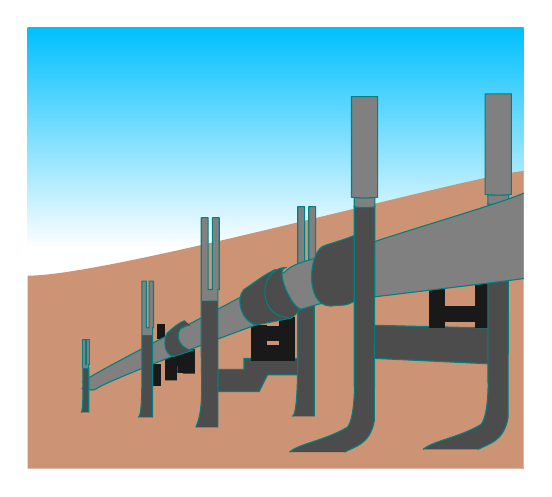
\begin{tikzpicture}[font=\footnotesize,scale=1,x=0.35cm,y=0.35cm]
			 \definecolor{antiquebrass}{rgb}{0.8,0.58,0.46}
			\definecolor{forestgreen  (web)}{rgb}{0.13,0.55,0.13}
			 \definecolor{deepskyblue}{rgb}{0.0,0.75,1.0}
			\fill[top color=deepskyblue,middle color=white] (-9,-7) rectangle (9,9); 
			\fill[antiquebrass](-9,0)..controls++(0:3)  and++(-175:2)..(9,3.8)--(9,-7)--(-9,-7)--cycle;
			\tikzset{ongdan/.pic={\draw[teal,fill=black!50]  (9,3)..controls++(-150:0.5) and++(25:0.4)..(3.5,1.2)..controls++(-130:0.4) and++(45:0.7)..(0.4,0.2)..controls++(-130:0.5) and++(40:0.7)..(-7,-3.85)..controls++(-10:0.4) and++(-170:0.3)..(-6.95,-4.1)..controls++(90:0.1) and++(-150:0.3)..(-6.5,-4.1)..controls++(40:0.5) and++(-170:1)..(1.7,-1)..controls++(10:0.3) and++(-170:0.5)..(9,-0.1);}}
			 \tikzset{cot/.pic={\draw[teal,fill=black!70] (0.5,-6.4)..controls++(40:0.5) and++(-150:1)..(2.6,-5.5)..controls++(50:0.5) and++(90:0.5)..(2.85,-4)--(2.85,2.5)..controls++(-10:0.2) and++(-170:0.2)..(3.6,2.5)..controls++(-90:0.5) and++(90:0.5)..(3.58,-5.25)..controls++(-100:0.9) and++(30:0.4)..(2.5,-6.4);
			 \draw[teal,fill=black!50] (2.85,2.5)..controls++(-10:0.2) and++(-170:0.2)..(3.6,2.5)--(3.6,2.85)..controls++(-170:0.2) and++(-10:0.2)..(2.85,2.85)--cycle;
			\draw[teal,fill=black!50] (3.7,2.85)..controls++(-170:0.2)  and++(-10:0.2)..(2.75,2.85)--(2.75,6.5)--(3.7,6.5)--cycle;}}
			\draw[teal,fill=black!70] (3.6,-1.8)--(7.8,-1.9)--(7.8,-3.2)--(3.6,-3); 
			\tikzset{cot1/.pic={\draw[teal,fill=black!70]  (-2.9,-5.6)..controls++(65:0.7) and++(-90:1)..(-2.7,-3)--(-2.7,-1)--(-2.1,-1)--(-2.1,-5.6);
			\draw[teal,fill=black!50](-2.7,-1)--(-2.7,2)..controls++(10:0.05) and++(170:0.05)..(-2.45,2)--(-2.45,-0.6)--(-2.3,-0.6)--(-2.3,2)..controls++(10:0.05) and++(170:0.05)..(-2.05,2)--(-2.05,-0.6)--(-2.1,-0.6)--(-2.1,-1);}} 
			\tikzset{cot2/.pic={\draw[teal,fill=black!70] (-2.9,-5.6)..controls++(8:0.2) and++(-90:1)..(-2.7,-3)--(-2.7,-1)--(-2.1,-1)--(-2.1,-5.6); 
			\draw[teal,fill=black!50](-2.7,-1)--(-2.7,2)..controls++(10:0.05) and++(170:0.05)..(-2.45,2)--(-2.45,-0.6)--(-2.3,-0.6)--(-2.3,2)..controls++(10:0.05) and++(170:0.05)..(-2.05,2)--(-2.05,-0.6)--(-2.1,-0.6)--(-2.1,-1);}} 
			\draw[teal,fill=black!70]  (-2.1,-3.4)--(-1.15,-3.4)--(-1.15,-3)--(1,-3)--(1,-3.6)--(-0.3,-3.6)--(-0.6,-4.2)--(-2.1,-4.2)--cycle;
			\draw[teal,black!90,line width=2mm] (0.4,-1.5)--(0.4,-2.8)--(-0.6,-2.8)--(-0.6,-1.8) 
				 (-0.6,-2.1)--(0.4,-2.1);
			\draw[teal,black!90,line width=2mm] (5.85,-0.5)--(5.85,-1.9) 
				 (7.5,-0.3)--(7.5,-1.9)
				(5.85,-1.4)--(7.5,-1.4); 
			\draw[teal,black!90,line width=1.5mm] (-3.8,-2.95)--(-3.8,-3.8) 
				 (-3.15,-2.66)--(-3.15,-3.55)
				(-3.35,-2.7)--(-3.35,-3.53) 
				 (-3.8,-3.1)--(-3.15,-3);
			 \draw[teal,black!90,line width=1mm] (-4.3,-4)--(-4.3,-3.2)
				(-4.15,-2.3)--(-4.15,-1.75); 
			\path (3.5,0.5) pic[scale=1]{cot2}; 
			 \path (4.85,0.1) pic[scale=1]{cot};
			\path (0,0)  pic[scale=1]{ongdan};
			\draw[teal,fill=black!70]  (1.8,1.1)..controls++(-170:0.6) and++(180:1)..(2,-1.1)..controls++(10:0.4) and++(-150:0.5)..(2.9,-0.9)..controls++(90:0.3) and++(-90:0.3)..(3.1,1.6)..controls++(-140:0.3) and++(20:0.3)..(1.8,1.1);
			\path (0,0.1) pic[scale=1]{cot1}; 
			 \path (-3.1,-1.5) pic[scale=0.65]{cot2};
			\path (0,0)  pic[scale=1]{cot};
			\path  (-6.05,-3) pic[scale=0.35]{cot2};
			\path (-6,1) node[rotate=12]{}; 
			\draw[teal,fill=black!70](0,0.23)..controls++(-155:0.4) and++(35:0.4)..(-1,-0.4)..controls++(-160:0.5)  and++(160:0.7)..(-0.73,-1.79)--(0.5,-1.55);
			\draw[teal,fill=black!70] (0.4,0.3)..controls++(180:1)  and++(170:1)..(0.3,-1.5)..controls++(0:0.2) and++(-130:0.7)..(0.9,-1.2)..controls++(180:0.3) and++(180:0.5)..(0.4,0.3);
			\draw[teal,fill=black!70]  (-3.1,-1.8)..controls++(180:0.7) and++(180:0.6)..(-3,-2.7)--(-3.7,-2.93)..controls++(170:0.4) and++(-120:0.2)..(-3.95,-2.1)..controls++(45:0.3) and++(-160:0.2)..(-3.3,-1.63);
			\path (6.5,0.8)  node[yellow,rotate=13]{};
		\end{tikzpicture}
	} 
	\noindent Với  hệ trục tọa độ $Oxyz$ thích hợp, đơn vị trên mỗi trục là mét, người ta thiết lập một đường ống dẫn dầu trên không dọc theo đường thẳng $d\colon
	\heva{&x=t\\&y=0\\&z=16}$ ($t$ là tham  số). Vì địa hình phức tạp, người ta đành chọn điểm $A(12;10;15)$ cạnh vách núi để làm điểm trung chuyển từ mặt đất (mặt phẳng $(Oxy)$) đến đường ống này. Dựa vào kinh nghiệm của mình họ phải chọn vị trí $B$ thuộc đường ống và vị trí $C$ thuộc mặt đất sao cho tổng độ dài các đoạn đường $AB$, $BC$, $AC$ là bé nhất, tìm giá trị bé nhất đó theo đơn vị mét, làm tròn đến hàng phần chục.
	 \shortans{42,6}
	 \loigiai{
		Vì điểm $A(12;10;15)$ và đường  thẳng $d$ cố định, nên khoảng cách từ $A$ đến $d$ không đổi.\\
		Vậy khoảng cách từ điểm $A$ đến điểm $B$ nhỏ nhất bằng khoảng cách  từ $A$ đến đường thẳng $d$.\\
		Gọi $(\alpha)$ là mặt  phẳng đi qua $A$ và vuông góc với $d$, $(\alpha)$ nhận $\overrightarrow{n}=(1;0;0)$ làm vectơ pháp tuyến $(\alpha)\colon x-12=0$.\\
		Khi đó $B$ là giao  điểm của đường thẳng $d$ và mặt phẳng $(\alpha)\Rightarrow B(12;0;16)$.\\
		Gọi $A'$ là điểm đối xứng của $A$ qua mặt phẳng $(Oxy)$ khi đó $A'(12;10;-15)$  và $CA=CA'$.\\
		Ta có  $AB+AC+BC=AB+BC+A'C$.\\
		Để tổng độ dài các đoạn đường  $AB$, $BC$, $AC$ là bé nhất.\\
		Suy ra $B$, $C$,  $A'$ thẳng hàng.\\
		Do đó $AB+BC+A'C=AB+BA'$.\\ 
		 Lại có $\overrightarrow{AB}(0;-10;1)$; $\overrightarrow{BA'}(12;10;-15)$.\\
		Vậy $AB+BC+A'C=AB+BA'=\sqrt{10^2+31^2}+\sqrt{10^2+1^2}\approx  42{,}6$.
	} 
\end{bt}


%%%%%%%%%%%%%%%% TỰ LUẬN %%%%%%%%%%%%%%%%

% nguồn: Phan2_Lop_12_Hinh_hoc_Chuong_5
\begin{bt}%[2H5H1-7]%[ma:ffc1432b]
	Ba chiếc máy bay không người lái cùng bay lên tại  một địa điểm. Sau một thời gian bay
	\begin{itemize}
		 \item Chiếc máy bay thứ nhất ở vị trí $A$ cách điểm xuất phát về phía Đông $60$ (km) và về phía Nam $40$ (km), đồng thời cách mặt đất $2$ (km).
		\item Chiếc máy bay thứ hai ở vị trí $B$ cách điểm xuất phát về phía Bắc $80$ (km), về phía Tây $50$ (km),  đồng thời cách mặt đất $4$ (km).
		\item Chiếc máy bay  thứ ba ở vị trí $I$ nằm chính giữa của chiếc máy bay thứ nhất và thứ hai, đồng thời ba chiếc máy bay này thẳng hàng.
	\end{itemize}
	Viết phương trình mặt phẳng $(P)$ đi qua  $I$ và vuông góc với đường thẳng $AB$.
	\loigiai{ 
	\immini{Chọn hệ trục tọa độ $Oxyz$, với gốc đặt tại điểm xuất phát của ba chiếc máy bay, mặt phẳng trùng với mặt đất, trục $Ox$ hướng về phía Bắc, trục $Oy$ hướng về phía Tây, trục $Oz$  hướng thẳng đứng lên trời, đơn vị đo lấy theo kilômét.
		Sau một thời gian bay }{ 
		\begin{tikzpicture}[scale=1,font=\footnotesize,line join=round,line cap=round,>=stealth]
				 \path
					 (0,0) coordinate (O)
					 (-2,-1) coordinate (A) node [below]{\text{ Bắc}}
					(4,0) coordinate (B)  node[right]{\text{ Tây}}
					($(O)!0.8!(A)$) coordinate  (x) node[above left]{$x$}
					($(O)!0.8!(B)$)  coordinate (y) node[above]{$y$}
					($(x)+(y)-(O)$) coordinate (m); 
				\draw[->] (O)--(A); 
				\draw[->]  (O)--(B);
				\draw[->] (O)--+(90:2)  node[above]{$z$};
				\draw[dashed]  (x)--(m)--(y);
			\end{tikzpicture}
		 }
		\begin{itemize}
			\item  Toạ độ chiếc máy bay thứ nhất là $A(-40;-60;2)$
			\item Toạ độ chiếc máy bay  thứ hai là $B(80;50;4)$
			\item Do chiếc máy bay thứ ba nằm chính giữa của chiếc máy bay thứ nhất và thứ hai, đồng thời ba chiếc máy bay này thẳng  hàng nên máy bay thứ ba ở vị trí trung điểm $I$ của $AB$, suy ra toạ độ chiếc máy bay thứ ba là $I(20;-5;3)$
		\end{itemize}
		Ta có $\vec{AB}=(120;110;2)\Rightarrow \vec{n}=(60;55;1)$  là vectơ pháp tuyến của $(P)$.\\
		Phương trình mặt  phẳng $(P)$ là
		$$60(x-20)+55(y+5)+(z-3)=0\Leftrightarrow 60x+55y+z-928=0$$ 
	 }
\end{bt}

% nguồn: Phan2_Lop_12_Hinh_hoc_Chuong_5
\begin{bt}%[2H5H1-7]%[ma:ce5904d6]
	Phần mềm của máy tiện kỹ  thuật số CNC (Computer Numerical Control) đang biểu diễn một chi tiết máy như Hinh $2$.
	\begin{enumerate}
		\item Tìm  toạ độ các điểm $A$, $B$, $C$, $D$.
		\item Viết phương trình mặt phẳng $(A  B C)$ và mặt phẳng $(ACD)$.
		\item  Viết phương trình tham số của đường thẳng $A C$.
		\item Cho  biết đầu mũi tiện đang đặt tại điêm $M(0; 60; 40)$. Tính khoảng cách từ $M$ đến mặt phẳng $(A B C)$
	\end{enumerate}
	 \loigiai{
		\begin{enumerate}
			\item Theo hình vẽ ta có toạ độ các điểm $A\left(70; 0; 0\right)$, $B\left(70; 0; -60\right)$,  $C\left(70; 80; 0\right)$, $D\left(50; 0; 0\right)$
			\item Ta có $\overrightarrow{AB}=\left(0; 0; -60\right)$, $\overrightarrow{AC}=\left(0;  80; 0\right)$.\\
			Mặt phẳng $(A B C)$ đi qua $A\left(70; 0; 0\right)$ và nhận $\left[\overrightarrow{AB},\overrightarrow{AC} \right]=\left(6400; 0; 0\right)$ làm  vectơ pháp tuyến.\\
			Phương trình $\left(ABC\right)$ là  $$6400\left(x-70\right)+0\left(y-0\right)+0\left(z-0\right)=0\Leftrightarrow x-70=0$$.
			Mặt phẳng $(A C D)$ đi qua $A\left(70; 0; 0\right)$ và nhận $\overrightarrow{k}=\left(0; 0; 1\right)$ làm vectơ pháp tuyến.\\  Phương trình $\left(A C D\right)$ là $z=0$.\\ Mặt phẳng $\left(ACD\right)$ cũng là mặt phẳng $\left(Oxy\right)$.
			\item Đường thẳng $A C$ đi qua điểm $A\left(70; 0; 0\right)$ và nhận $\overrightarrow{AC}=\left(0; 80; 0\right)$ làm vectơ chỉ phương. Phương trình tham số  của đường thẳng $AC$ là $\heva{&x=70\\&y=t\\&z=0}$.
			\item Khoảng cách từ $M$ đến  mặt phẳng $(A B C)$ là $\mathrm{d}\left(M,\left(A B C\right)\right)=\dfrac{\left|0-70 \right| }{\sqrt{1^2+0^2+0^2}}=70$.
		\end{enumerate}
	} 
\end{bt}

% nguồn: Phan2_Lop_12_Hinh_hoc_Chuong_5
\begin{bt}%[2H5H1-7]%[ma:bfd11348]
	Trong không gian $Oxyz$, một ngôi nhà có sàn nhà thuộc mặt phẳng $Oxy$ và trần nhà tầng $1$ thuộc mặt phẳng $z-1=0$, mái nhà tầng $2$ thuộc mặt phẳng $x+y+50z-100=0$. Hỏi trong $3$ mặt phẳng tương  ứng chứa sàn nhà, trần nhà tầng $1$, mái nhà tầng $2$, hai mặt nào song song với nhau?
	 \loigiai{
		Vì mặt phẳng $Oxy$ vuông góc với $Oz$ nên mặt phẳng $Oxy$ nhận $\vec{k}=(0; 0; 1)$ làm một vectơ pháp  tuyến.\\
		Vì mặt phẳng $Oxy$ đi qua điểm $O(0; 0; 0)$ và có vectơ pháp tuyến $\vec{k}=(0; 0; 1)$ nên  có phương trình là $z-0=0\Leftrightarrow z=0$.\\
		Mặt phẳng $z-1=0$  có vectơ pháp tuyến là $\overrightarrow{n}_1=(0; 0; 1)$.\\
		Vì $\overrightarrow{n}_1=\vec{k}$  và $-1\neq 0$ nên mặt phẳng chứa sàn nhà song song với trần tầng $1$.\\
		Mặt mái tầng $2$ có phương trình $x+y+50z-100=0$ và có nhận một vectơ pháp tuyến là $\overrightarrow{n}_2=(1; 1; 50)$ không cùng phương với $\overrightarrow{n}_1$, $\vec{k}$ nên không song song với hai mặt  phẳng còn lại.
	} 
\end{bt}

% nguồn: Ok_TuanLuan_Toan11_Lan2
\begin{ex}%[2H5V1-7]%[ma:44564a6c]
	Trong không gian $Oxyz$ (đơn vị trên mỗi trục tọa độ là mét), một ngôi nhà có sàn nhà nằm trên mặt phẳng $(Oxy)$. Hai mái nhà lần lượt nằm trên các mặt phẳng $(P)\colon x-2y+5=0$ và $(Q)\colon x-2y-3z+20=0$. Hỏi là chiều cao của ngôi nhà tính  từ sàn nhà lên nóc nhà (điểm cao nhất của mái nhà) là bao nhiêu?
	\loigiai{ 
		Những điểm thuộc đường  nóc nhà có tọa độ thỏa mãn hệ $\heva{&x-2y+5=0\\&x-2y-3z+20=0.}$\\
		Từ phương trình thứ nhất chọn $x=-5\Rightarrow  y=0$.\\
		Thay vào phương trình còn  lại ta được $z=5$.\\
		Vậy điểm $A(-5;0;5)$ là một điểm  thuộc đường nóc nhà.\\
		Khi  đó chiều cao cần tìm của của ngôi nhà là khoảng cách từ điểm $A$ đến mặt phẳng $(Oxy)$ và bằng $5$ mét.
	} 
\end{ex}

% nguồn: Ok_TuanLuan_Toan11_Lan2
\begin{ex}%[2H5V1-7]%[ma:7a353a49]
	Phần mềm điều khiển máy in 3D cho biết đầu in phun của máy đang đặt tại điểm $M(3;4;24)$ (đơn vị: cm). Tính khoảng cách từ đầu in đến khay đặt vật in có phương  trình $z-4=0$.
	 \loigiai{
		Ta  có phương trình mặt phẳng là $(P)\colon z-4=0$.\\
		Khoảng cách từ đầu  in đến khay đặt vật in là $\mathrm{d}\Big(M,(P)\Big)=\dfrac{\left|24-4\right|}{1}=20$.
	} 
\end{ex}

% nguồn: Ok_TuanLuan_Toan11_Lan2
\begin{ex}%[2H5V1-7]%[ma:56d404ba]
	\immini[thm]{Một phần sân trường được định vị bởi các điểm $A$, $B$, $C$, $D$ như hình vẽ. Bước đầu chúng được lấy \lq\lq thăng bằng\rq\rq \ \ để có cùng độ cao, biết $ABCD$ là hình thang vuông ở $A$ và $B$ với độ dài $AB=25$\,m, $AD=15$\,m, $BC=18$\,m. Do yêu cầu kĩ thuật, khi lát phẳng phàn  sân trường phải thoát nước về góc sân ở $C$ nên người ta lấy độ cao ở các điểm $B$, $C$, $D$ xuống thấp hơn so với độ cao ở $A$ là $10$\,cm, $a$\,cm, $6$\,cm tương ứng. Giá trị của $a$ bằng bao nhiêu?
	}{ 
	\begin{tikzpicture}[thick]
			\coordinate (A)  at (0,0);
			\coordinate (B) at (3.75,0); 
			\coordinate (D) at  (0,-2.25);
			\coordinate (C)  at (3.75,-2.7);
			\fill[gray!30] (A) -- (B) -- (C) --  (D) -- cycle;
			\draw(A) -- (B)  -- (C) -- (D) -- cycle;
			\node[above left]  at (A) {$A$};
			\node[above right] at (B) {$B$}; 
			 \node[below right] at (C) {$C$};
			\node[below left] at  (D) {$D$};
			\node[above] at ($(A)!0.5!(B)$)  {$25$\,m};
			 \node[left] at ($(A)!0.5!(D)$) {$15$\,m};
			\node[right] at  ($(B)!0.5!(C)$) {$18$\,m};
		\end{tikzpicture}
	 }
	 \loigiai{
		\begin{center}
			\begin{tikzpicture}[line join=round,line cap=round,>=stealth]
					 \coordinate (A) at (0,0);
					\coordinate  (y) at ($(A)+(0:5)$);
					\coordinate (z) at  ($(A)+(90:2)$);
					\coordinate (x) at  ($(A)+(-120:3)$);
					 \coordinate (B) at ($(A)+(0:4)$);
					\coordinate  (C) at ($(A)+(-40:3)$);
					 \coordinate (D) at ($(A)+(-120:1.5)$);
					 \coordinate (B') at ($(B)+(-90:1)$);
					\coordinate (C')  at ($(C)+(-90:1)$);
					\coordinate  (D') at ($(D)+(-90:1)$);
					\draw[->] (A) -- (x) node[left]  {$x$};
					 \draw[->] (A) -- (y) node[below] {$y$};
					\draw[->] (A) -- (z) node[left] {$z$}; 
					\draw  (B)--(C)--(D);
					\draw [dashed](D)--(D')--(C')--(C) 
						 (C')--(B')--(B);
					\foreach \i/\g in {A/180,B/90,C/100,D/180,B'/0,C'/-90,D'/-90}{\draw[fill](\i)  circle (1pt)
						($(\i)+(\g:3mm)$)  node[scale=1]{$\i$};}
				\end{tikzpicture}
		\end{center}
		Chọn hệ trục  tọa độ $Oxyz$ sao cho $O\equiv A$, tia $Ox\equiv AD$, tia $ Oy\equiv AB$.\\
		Khi  đó $A(0;0;0)$; $B(0;2\,500;0)$; $C(1\,800;2\,500;0)$; $D(1\,500;0;0)$.\\
		Khi hạ độ cao các điểm  ở các điểm $B$, $C$, $D$ xuống thấp hơn so với độ cao ở $A$ là $10$\,cm; $a$\,cm; $6$\,cm tương ứng ta có các điểm mới $B'(0;2\,500;-10)$; $C'(1\,800;2\,500;-a)$; $D'(1\,500;0;-6)$.\\
		Theo  bài ra có bốn điểm $A$; $B'$; $C'$; $D'$ đồng phẳng.\\
		Phương trình mặt phẳng  $(AB'D')\colon x+y+250z=0$.\\
		Do $C'(1\,800;2\,500;-a)\in (AB'D')$  nên ta có $1\,800+2\,500-250a=0\Leftrightarrow a=17{,}2$\,cm.\\
		Vậy $a=17{,}2$. 
	} 
\end{ex}

% nguồn: Ok_TuanLuan_Toan11_Lan2
\begin{ex}%[2H5V1-7]%[ma:7742a6b8]
	\immini[thm]{Một sân vận động được xây dựng theo mô hình là hình chóp cụt $OAGD.BCFE$ có hai đáy song song với nhau. Mặt sân $OAGD$ là hình chữ nhật và được gắn hệ trục $Oxyz$ như hình vẽ (đơn vị trên mỗi trục tọa độ là mét). Mặt sân $OAGD$ có chiều dài $OA=100$\,m, chiều rộng $OD=60$\,m và tọa độ điểm $B(10;10;8)$. Giả sử phương trình tổng quát của mặt phẳng $(OACB)$ có dạng $ax+y+cz+d=0$. Tính giá trị biểu thức $a+c+d$. 
	 }{
	\begin{tikzpicture}[>=stealth,scale=0.8]
			\coordinate  (O) at (0,0);
			 \coordinate (A) at (3.75,1.875);
			 \coordinate (D) at (-2,2);
			 \coordinate (G) at (1.5,3);
			\coordinate (B)  at ($(O)+(0.5,1.5)$);
			\coordinate (E) at ($(B)+(-1.6,1.6)$); 
			\coordinate (F) at  ($(E)+(2.8,0.8)$);
			 \coordinate (C) at ($(B)+(3.2,1.6)$);
			\fill[gray!10] (O)--(D)--(G)--(A)--cycle; 
			\fill[gray!40]  (D)--(E)--(F)--(G)
				(G)--(F)--(C)--(A); 
			\draw[->] (O) -- (4.5,2.25)  node[below] {$x$};
			 \draw[->] (O) -- (-2.5,2.5) node[left] {$y$};
			\draw[->] (O) --  (0,3) node[left] {$z$};
			\draw (O)  -- (A)
				(O)  -- (D)
				(B)--(C)--(F)--(E)--cycle (D)--(E) 
				(O)--(B) 
				(A)--(C); 
			 \draw[dashed](D)--(G)--(A)
				(G)--(F); 
			\foreach  \i/\g in {O/-90,A/-60,D/200,G/-110,B/-40,F/30,E/90,C/30}{\draw[fill](\i) circle (1pt)
				($(\i)+(\g:3.5mm)$)  node[scale=0.8]{$\i$};}
		\end{tikzpicture}
	} 
	\loigiai{ 
		Gắn hình chóp cụt vào hệ trục $Oxyz$  ta có $O(0;0;0)$, $A(100;0;0)$, $G(100;60;0)$, $D(0;60;0)$, $B(10;10;8)$.\\
		Do $\overrightarrow{OA}=(100;0;0)$, $\overrightarrow{OB}=(10;10;8)$  nên $\overrightarrow{n}=\left[\overrightarrow{OA},\overrightarrow{OB}\right]=(0;-100;1000)$.\\
		Suy ra mặt phẳng $(OACB)$ có véc-tơ pháp tuyến là $\overrightarrow{n}_1=(0;1;-10)$.\\ 
		Phương  trình tổng quát của mặt phẳng $(OACB)$ là $y-10z=0$ .\\
		Do đó $a=0$,  $c=-10$, $d=0$.\\
		 Vậy $a+c+d=0-10+0=-10$.
	 }
\end{ex}

% nguồn: Ok_TuanLuan_Toan11_Lan2
\begin{ex}%[2H5V1-7]%[ma:256dd61d]
	Một khu nhà đang được xây dựng, được gắn hệ trục tọa độ $Oxyz$ (đơn  vị trên các trục là mét). Mỗi cột bê tông có dạng hình lăng trụ tứ giác đều cạnh đáy dài $1$\,m và tâm của mặt đáy trên lần lượt là các điểm $A(2;1;3)$, $B(4;3;3)$, $C(6;3;3)$, $D(4;0;2{,}5)$. Giám sát công trình tính toán nhận thấy $A$, $B$, $C$, $D$ không đồng phẳng, yêu cầu bên nhà thầu tính khối lượng bê tông cần bổ sung để độ cao các cột bê tông bằng nhau. Tính thể tích bê tông cần bổ sung (giả sử thể tích phần cốt thép là $3\%$ trên một mét khối bê tông).
	 \loigiai{
		 Ta có $\overrightarrow{AB}=(2;2;0)$, $\overrightarrow{AC}=(4;2;0)\Rightarrow \left[\overrightarrow{AB},\overrightarrow{AC}\right]=(0;0;-4)$.\\
		 Phương trình $(ABC)$ đi qua $A(2;1;3)$ và nhận $\overrightarrow{n}=\left[\overrightarrow{AB},\overrightarrow{AC}\right]=(0;0;-4)$ làm một véctơ pháp tuyến là $-4(z-3)=0\Leftrightarrow z-3=0$.\\
		Khoảng cách từ $D$ đến mặt phẳng  $(ABC)$ là $\mathrm{d}\Big(D,(ABC)\Big)=\dfrac{\left|2{,}5-3\right|}{1}=0{,}5$\,(m).\\
		Vì mỗi cột bê tông  là hình lăng trụ tứ giác đều và thể tích phần cốt thép là $3\%$ trên một mét khối bê tông, do đó thể tích phần bê tông cần bổ sung là
		\[V=1\cdot 1\cdot 0{,}5(100-3)\%=0{,}5\cdot  97\%=0{,}485\,(\text{m}^3).\]
	 }
\end{ex}

% nguồn: Ok_TuanLuan_Toan11_Lan2
\begin{ex}%[2H5V1-7]%[ma:16eb9874]
	Trong tiết thể dục học về kĩ thuật chuyền bóng hơi, Nam và An đang tập chuyền bóng cho nhau, Nam ném bóng cho An đỡ, quả bóng bay lên cao nhưng lại lệch sang phải của Nam và rơi xuống vị trí cách An $0{,}5$\,m và cách  Nam $4{,}5$\,m được mô tả bằng hình vẽ bên dưới
	\begin{center}
		\begin{tikzpicture}[scale=.7,>=stealth,line join=round,line cap=round,font=\footnotesize]
				\path (0,0)  coordinate (O) coordinate (peo)
					 +(0:1) coordinate (i)
					 +(-135:2.5) coordinate (j)
					+(90:1) coordinate (k) 
					($4.472*(i)$) coordinate (M) coordinate (pe) 
					($4.472*(i)+.5*(j)$) coordinate (N); 
				\begin{scope}[scale=.45]
					\draw  [fill] (pe) ++(-.34,.26).. controls +(-.58,-.19) and +(-.61,-.03).. ++(.34,-.26)
						.. controls  +(.05,.13) and +(.11,-.03).. ++(-.11,.26)
						(pe)++(.85,.24).. controls +(.21,-.08) and +(-.48,-.26).. ++(.26,-.19) 
						.. controls  +(.16,.13) and +(.24,-.11).. ++(-.05,.37)
						(pe)++(.9,1.16).. controls  +(.26,.26).. ++(.08,.5)
						.. controls +(-.19,-.13) and +(.13,-.03).. ++(-.56,-.05) 
						.. controls +(-.03,-.13) and  +(-.08,.11).. ++(-.24,-.16)
						.. controls +(-.05,-.13) and  +(-.13,.16).. cycle
						(pe)++(.37,2.54).. controls +(-.16,.03) and +(.19,.05).. ++(-.56,.26) 
						.. controls +(.11,.24) and +(.11,.61)..  cycle;
					\draw  [fill=gray!20] (pe)++(-.11,.26)
						.. controls  +(-.03,.85) and +(-.42,-.24).. ++(.48,.95)
						.. controls  +(-.32,-.5) and +(-.79,.48).. ++(.48,-.98)--++(.21,.19)
						.. controls +(-.63,.37) and +(-.37,-.26)..  ++(-.16,.73)
						.. controls +(-.13,.16)  and +(-.05,-.13).. ++(-.71,.29)
						.. controls +(-.82,-.24) and  +(-.11,.69).. ++(-.53,-1.19)
						(pe)++(.98,1.67).. controls +(.11,.34)  and +(.32,-.16).. ++(-.61,.87)
						.. controls  +(-.19,-.26).. ++(-.45,-.11)
						.. controls +(-.26,-.48) and  +(.56,.58).. ++(-.66,-1.32)
						.. controls  +(.16,-.34) and +(-.11,-.42).. ++(.74,.82)
						.. controls +(.24,.13)..  ++(.21,-.13)
						 .. controls +(.19,.21) and +(.19,.16).. ++(.21,-.19)
						 .. controls +(.13,-.03) and +(-.19,-.13).. cycle
						(pe)++(.37,2.54).. controls +(-.16,.03) and  +(.19,.05).. ++(-.56,.26)
						.. controls +(-.11,-.11) and +(-.13,.08)..  ++(.11,-.37)
						.. controls +(.26,-.16).. cycle; 
					\draw [fill=gray!20](pe)++(.21,1.8).. controls  +(-.03,-.19) and +(.43,.23).. ++(-.45,-.41)
						.. controls  +(-.95,-.67) and +(-.5,-.58).. ++(.67,.23);
				\end{scope}
				\begin{scope}[scale=.3]
					\draw [fill] (peo).. controls +(1.08,-.13) and +(.03,-.29)..  ++(.16,.45)--++(-.32,0)
						.. controls +(-.37,-.34) and +(-.45,-.08)..  cycle
						(peo)++(-1.53,.56).. controls +(-.21,.08) and  +(0,.85).. ++(-.4,-.69)
						.. controls +(.29,-.11)  and +(.03,-.66).. cycle
						(peo)++(.48,2.17)..  controls +(-.66,-.13).. ++(-1.27,-.03)
						.. controls +(0,.61).. ++(.24,.85) 
						..  controls +(.42,-.11).. ++(.9,0)
						.. controls  +(.26,-.45).. cycle
						(peo)++(-.56,4.8).. controls +(-.29,.12)  and +(-.77,-.5).. ++(-.08,.92)
						..  controls +(.4,.11) and +(.26,.13).. ++(.13,-.24)
						.. controls +(-.26,-.24) and +(-.18,.17)..  ++(.15,-.54)--cycle;
					\draw [fill=gray!20] (peo)++(-.35,4.93).. controls +(-.18,.17) and +(-.26,-.24)..  ++(-.15,.54)
						 .. controls +(.24,.24) and +(-.03,.48).. ++(.45,-.53)--cycle;
					\draw [fill=gray!20] (peo)++(.16,.45).. controls  +(.34,1.03) and +(.19,-.37).. ++(.32,1.72)
						.. controls  +(-.66,-.13).. ++(-1.27,-.03)
						.. controls +(.03,-.69) and +(.06,1).. ++(-1.04,-1.6) 
						.. controls +(.48,-.04) and +(-.5,-.79).. ++(1.78,1.71) 
						.. controls +(.13,-.56) and ++(-.11,.58)..  ++(-.11,-1.8)--cycle
						(peo)++(.34,2.99).. controls  +(.24,.77) and +(.4,-.03).. ++(-.32,1.61)
						.. controls  +(.79,.74) and +(.11,-.56).. ++(1.27,1.88) coordinate (bo)
						.. controls +(-.11,.34) and +(0,.66).. ++(-.34,-.26) 
						.. controls +(-.05,-.32)  and +(.69,.77).. ++(-1.01,-1.27)
						.. controls +(-.24,.16) and  +(-.21,.34).. ++(-.69,-.69)
						..  controls +(.21,-.24) and +(.03,.56).. ++(.19,-1.27)
						..  controls +(.42,-.11).. cycle;
				\end{scope}
				 \draw [->] (O)--($6*(i)$) node [below,xshift=-3pt] {$x$};
				\draw [->] (O)--(j) node [left]  {$y$};
				\draw [->] (O)--($4*(k)$) node [left,yshift=-4pt] {$z$}; 
				\draw [fill] (0,0) circle (1pt)  node [below] {$O$}
					 (N) circle (1pt)
					 (M) circle (1pt)
					 (bo) circle (.15);
				 \draw (O)--(N) node [midway,sloped,below] {$4{,}5$ m};
				\draw [densely  dashed] (N)--(M) node [midway,sloped,below] {$0{,}5$ m}
					 (bo).. controls +(60:2.5) and +(100:3).. (N);
			\end{tikzpicture}
	\end{center}
	Biết rằng quỹ đạo của quả bóng nằm trong mặt phẳng $(\alpha)\colon ax+\dfrac{1}{2}y+cx+d=0$ và vuông góc với mặt đất. Khi  đó giá trị của $a+c+d$ bằng (kết quả làm tròn đến hàng phần chục).
	\loigiai{ 
		\begin{center}
			\begin{tikzpicture}[scale=.7,>=stealth,line join=round,line cap=round,font=\footnotesize]
					\path (0,0) coordinate (O)  coordinate (peo)
						+(0:1)  coordinate (i)
						 +(-135:2.5) coordinate (j)
						+(90:1) coordinate  (k)
						($4.472*(i)$) coordinate (M) coordinate  (pe)
						($4.472*(i)+.5*(j)$) coordinate (N); 
					\begin{scope}[scale=.45]
						\draw [fill] (pe) ++(-.34,.26).. controls +(-.58,-.19) and +(-.61,-.03).. ++(.34,-.26) 
						.. controls +(.05,.13)  and +(.11,-.03).. ++(-.11,.26)
						(pe)++(.85,.24)..  controls +(.21,-.08) and +(-.48,-.26).. ++(.26,-.19)
						.. controls +(.16,.13) and  +(.24,-.11).. ++(-.05,.37)
						(pe)++(.9,1.16).. controls +(.26,.26).. ++(.08,.5) 
						.. controls +(-.19,-.13) and  +(.13,-.03).. ++(-.56,-.05)
						.. controls +(-.03,-.13) and +(-.08,.11).. ++(-.24,-.16) 
						.. controls  +(-.05,-.13) and +(-.13,.16).. cycle
						(pe)++(.37,2.54)..  controls +(-.16,.03) and +(.19,.05).. ++(-.56,.26)
						 .. controls +(.11,.24) and +(.11,.61).. cycle;
						 \draw [fill=gray!20] (pe)++(-.11,.26)
						..  controls +(-.03,.85) and +(-.42,-.24).. ++(.48,.95)
						.. controls +(-.32,-.5) and +(-.79,.48).. ++(.48,-.98)--++(.21,.19) 
						.. controls +(-.63,.37) and +(-.37,-.26)..  ++(-.16,.73)
						.. controls +(-.13,.16)  and +(-.05,-.13).. ++(-.71,.29)
						.. controls  +(-.82,-.24) and +(-.11,.69).. ++(-.53,-1.19)
						(pe)++(.98,1.67).. controls +(.11,.34)  and +(.32,-.16).. ++(-.61,.87)
						.. controls  +(-.19,-.26).. ++(-.45,-.11)
						..  controls +(-.26,-.48) and +(.56,.58).. ++(-.66,-1.32)
						..  controls +(.16,-.34) and +(-.11,-.42).. ++(.74,.82)
						.. controls +(.24,.13).. ++(.21,-.13) 
						 .. controls +(.19,.21) and +(.19,.16).. ++(.21,-.19)
						.. controls +(.13,-.03)  and +(-.19,-.13).. cycle
						(pe)++(.37,2.54).. controls +(-.16,.03) and +(.19,.05).. ++(-.56,.26) 
						 .. controls +(-.11,-.11) and +(-.13,.08).. ++(.11,-.37)
						 .. controls +(.26,-.16).. cycle;
						\draw [fill=gray!20](pe)++(.21,1.8).. controls  +(-.03,-.19) and +(.43,.23).. ++(-.45,-.41)
						.. controls +(-.95,-.67) and  +(-.5,-.58).. ++(.67,.23);
					\end{scope}
					\begin{scope}[scale=.3]
						\draw [fill] (peo).. controls  +(1.08,-.13) and +(.03,-.29).. ++(.16,.45)--++(-.32,0)
						.. controls +(-.37,-.34) and +(-.45,-.08).. cycle 
						(peo)++(-1.53,.56)..  controls +(-.21,.08) and +(0,.85).. ++(-.4,-.69)
						.. controls +(.29,-.11) and +(.03,-.66)..  cycle
						(peo)++(.48,2.17).. controls +(-.66,-.13).. ++(-1.27,-.03) 
						.. controls +(0,.61).. ++(.24,.85) 
						.. controls +(.42,-.11)..  ++(.9,0)
						.. controls +(.26,-.45)..  cycle
						(peo)++(-.56,4.8).. controls  +(-.29,.12) and +(-.77,-.5).. ++(-.08,.92)
						.. controls  +(.4,.11) and +(.26,.13).. ++(.13,-.24)
						.. controls +(-.26,-.24) and +(-.18,.17)..  ++(.15,-.54)--cycle;
						\draw  [fill=gray!20] (peo)++(-.35,4.93).. controls +(-.18,.17) and +(-.26,-.24).. ++(-.15,.54)
						.. controls +(.24,.24) and +(-.03,.48)..  ++(.45,-.53)--cycle;
						\draw [fill=gray!20] (peo)++(.16,.45).. controls +(.34,1.03)  and +(.19,-.37).. ++(.32,1.72)
						..  controls +(-.66,-.13).. ++(-1.27,-.03)
						.. controls +(.03,-.69) and +(.06,1).. ++(-1.04,-1.6) 
						.. controls +(.48,-.04) and +(-.5,-.79).. ++(1.78,1.71) 
						 .. controls +(.13,-.56) and ++(-.11,.58).. ++(-.11,-1.8)--cycle
						(peo)++(.34,2.99).. controls +(.24,.77) and +(.4,-.03).. ++(-.32,1.61) 
						 .. controls +(.79,.74) and +(.11,-.56).. ++(1.27,1.88) coordinate (bo)
						.. controls  +(-.11,.34) and +(0,.66).. ++(-.34,-.26)
						.. controls +(-.05,-.32) and +(.69,.77)..  ++(-1.01,-1.27)
						.. controls +(-.24,.16) and +(-.21,.34).. ++(-.69,-.69) 
						.. controls +(.21,-.24)  and +(.03,.56).. ++(.19,-1.27)
						.. controls +(.42,-.11)..  cycle;
					\end{scope}
					\draw [->] (O)--($6*(i)$)  node [below,xshift=-3pt] {$x$};
					\draw [->]  (O)--(j) node [left] {$y$};
					\draw [->] (O)--($4*(k)$) node [left,yshift=-4pt]  {$z$};
					\draw [fill]  (0,0) circle (1pt) node [below] {$O$}
						(N) circle (1pt) 
						(M) circle (1pt) 
						(bo)  circle (.15);
					\draw (O)--(N) node [midway,sloped,below] {$4{,}5$ m}; 
					\draw [densely dashed] (N)--(M) node [midway,sloped,below]  {$0{,}5$ m}
						(bo).. controls +(60:2.5) and +(100:3).. (N); 
				\end{tikzpicture}
		\end{center}
		Chọn hệ trục như hình vẽ. Gọi $M$  là điểm mà quả bóng chạm đất.\\
		Khi đó  $x_M=0{,}5$, $y_M=\sqrt{4{,}5^2-0{,}5^2}=2\sqrt{5}$.\\
		Vì $(\alpha)\perp(Oxy)$ nên $(\alpha)$ có véc-tơ  chỉ phương $\overrightarrow{k}=(0;0;1)$.\\
		Mà $(\alpha)$ có véc-tơ chỉ  phương $\overrightarrow{OM}=(0{,}5;2\sqrt 5;0)$.\\
		Khi  đó vec tơ pháp tuyến của $(\alpha)$ là $\overrightarrow{n}_{\alpha}=\left[\overrightarrow{k},\overrightarrow{OM}\right]=(-2\sqrt{5};0{,}5;0)$.\\
		Suy ra  $(\alpha)\colon -2\sqrt{5}x+0{,}5y=0$ nên $a=-2\sqrt{5}$; $b=0{,}5$; $c=0$; $d=0$.\\
		Vậy  $a+b+c+d\approx -4{,}5$.
	 }
\end{ex}

% nguồn: Ok_TuanLuan_Toan11_Lan2
\begin{ex}%[2H5V1-7]%[ma:036a2e32]
	Một ngôi nhà có các bậc thang của cầu thang đã thiết lập hệ tọa độ  $Oxyz$. Biết hai mặt bậc thang song song nằm trên hai mặt phẳng phân biệt $(P)\colon 2x-y+2z+8=0$ và $(Q)\colon 2x-y+2z+2=0$. Khoảng cách giữa hai bậc thang này bằng bao nhiêu?
	\loigiai{ 
		Khoảng cách giữa hai bậc  thang này bằng khoảng cách giữa hai mặt phẳng $(P)$ và $(Q)$ là
		 \[\mathrm{d}\Big((P),(Q)\Big)=\dfrac{\left|2-8\right|}{\sqrt{2^2+(-1)^2+2^2}}=\dfrac{6}{3}=2.\]
		Vậy khoảng cách giữa hai bậc  thang bằng $2$.
	 }
\end{ex}

% nguồn: Ok_TuanLuan_Toan11_Lan2
\begin{ex}%[2H5V1-7]%[ma:1ecb38f8]
	\immini[thm]{Phần mềm của máy tiện kĩ thuật số CNC (Computer Numerical Control) đang biểu diễn một chi tiết máy như hình  vẽ
	\begin{enumerate}[a)]
		\item  Tìm tọa độ các điểm $A$, $B$, $C$, $D$.
		\item Viết phương trình mặt phẳng $(ABC)$  và mặt phẳng $(ACD)$.
		\item Cho biết đầu mũi tiện đang đặt tại điểm $M(0;60;40)$. Tính khoảng  cách từ điểm $M$ đến mặt phẳng $(ABC)$.
	\end{enumerate}
	}{ 
	\begin{tikzpicture}[line join = round,line cap = round,>=stealth,font=\footnotesize,scale=.65]
			\coordinate  (0) at (0,0);
			\def \gocx{-20} 
			 \def \gocy{25}
			 \def \gocz{90}
			\def \xp{8}  \def \yp{10}\def \zp{5}
			 \def \xt{-3}\def \yt{-3}\def \zt{-7}
			\def \scalex{0.7} \def \scaley{0.7}  \def \scalez{0.6}
			\draw[->]({\gocx+180}:{-\xt*\scalex})--({\gocx}:{\xp*\scalex}) node[below]{$x$}; 
			\draw[->] ({\gocy+180}:{-\yt*\scaley})--({\gocy}:{\yp*\scaley}) node[below]{$y$}; 
			 \draw[->]({\gocz+180}:{-\zt*\scalez})--({\gocz}:{\zp*\scalez}) node[left]{$z$};
			\coordinate (i) at  ({\gocx}:{\scalex});
			\coordinate  (j) at ({\gocy}:{\scaley});
			\coordinate  (k) at ({\gocz}:{\scalez});
			\fill  (0,0) circle (1pt) node[below left]{$0$};
			\foreach  \x/\y/\z/\diem in
				{2/8/0/P,0/8/4/M,2/0/-2/Q,2/8/-2/R,5/0/-2/S,5/8/0/T,7/8/0/C,7/0/0/A,7/0/-6/B,7/8/-6/U,5/8/-2/V,5/0/0/D} 
				 {
			\coordinate  (\diem1) at ($(0)!\x!(i)$);
			 \coordinate (\diem2) at ($(0)!\y!(j)$);
			\coordinate  (\diem3) at ($(0)!\z!(k)$);
			\coordinate (\diem)  at ($($(\diem1)+(\diem2)-(0)$)+(\diem3)-(0)$);
			} 
			 \foreach \x/\goc in {-2/90,2/90,5/-135,7/90}\fill($(0)!\x!(i)$) circle (1pt)
				($($(0)!\x!(i)$)+(\goc:4mm)$) node{$\x0$}; 
			\foreach \y  in {-2,2,4,6,8}\fill($(0)!\y!(j)$) circle (1pt)
				($($(0)!\y!(j)$)+(120:4mm)$) node{$\y0$}; 
			\foreach \z in  {-6,-4,-2,2,4}\fill($(0)!\z!(k)$) circle (1pt)
				($($(0)!\z!(k)$)+(180:5mm)$) 
				node{$\z0$}; 
			\coordinate  (X) at (intersection of R--V and T--D);
			 \draw(0)--(M2)--(P)--(P1)--cycle (P1)--(Q)--(R)--(P)
				 (Q)--(S)--(S1)--(T)--(C)--(A)--(B)--(B3)--(0)
				(B)--(U)--(C) 
				 (R)--(X);
			 \draw[dashed] (M2)--(M)--(M3);
			\foreach \diem/\goc  in {M/0,D/-45,A/-135,B/135,C/90
				}  \fill(\diem) circle (1pt)
				($(\diem)+(\goc:3mm)$) node{$\diem$}; 
		\end{tikzpicture}
	} 
	 \loigiai{
		\begin{enumerate}[a)]
			\item Ta  có $A(70;0;0)$, $B(70;0;-60)$, $C(70;80;0)$, $D(50;0;0)$.
			\item Mặt phẳng $(ABC)$ đi qua $A(70;0;0)$ và vuông góc với trục $Ox$ nên có véc-tơ  pháp tuyến là $\overrightarrow{i}=(1;0;0)$.\\
			 Suy ra mặt phẳng $(ABC)$ có phương trình là $1(x-70)=0\Leftrightarrow x-70=0$.\\
			Mặt phẳng $(ACD)$ đi qua $A(70;0;0)$ và vuông góc với trục $Oz$ nên có véc-tơ pháp  tuyến là $\overrightarrow{k}=(0;0;1)$.\\
			Suy ra mặt phẳng $(ACD)$ có phương trình là $1(z-0)=0\Leftrightarrow  z=0$.
			\item Khoảng cách từ điểm $M$ đến mặt phẳng $(ABC)$ là  $\mathrm{d}\Big(M,(ABC)\Big)=\dfrac{\left|0-70\right|}{1}=70$.
		\end{enumerate}
	} 
\end{ex}

% nguồn: Phan2_Lop_12_Hinh_hoc_Chuong_5
\begin{bt}%[2H5V1-7]%[ma:6d18ed58]
	Trong tiết thể dục học về kĩ thuật chuyền bóng hơi, Nam và An đang tập chuyền bóng cho nhau, Nam ném bóng cho An đỡ, quả bóng bay lên cao nhưng lại lệch sang phải của Nam và rơi  xuống vị trí cách An $0{,}5$\,m và cách Nam $4{,}5$\,m được mô tả bằng hình vẽ bên dưới
	\begin{center}
		\begin{tikzpicture}[scale=.7,>=stealth,line join=round,line cap=round,font=\footnotesize]
				 \path (0,0) coordinate (O) coordinate (peo)
					+(0:1)  coordinate (i)
					+(-135:2.5) coordinate  (j)
					+(90:1) coordinate (k) 
					($4.472*(i)$) coordinate (M) coordinate  (pe)
					($4.472*(i)+.5*(j)$)  coordinate (N);
				\begin{scope}[scale=.45]
					 \draw (pe) ++(-.34,.26).. controls +(-.58,-.19) and +(-.61,-.03).. ++(.34,-.26)
						.. controls  +(.05,.13) and +(.11,-.03).. ++(-.11,.26)
						(pe)++(.85,.24).. controls +(.21,-.08) and +(-.48,-.26).. ++(.26,-.19) 
						..  controls +(.16,.13) and +(.24,-.11).. ++(-.05,.37)
						(pe)++(.9,1.16).. controls +(.26,.26)..  ++(.08,.5)
						.. controls  +(-.19,-.13) and +(.13,-.03).. ++(-.56,-.05)
						 .. controls +(-.03,-.13) and +(-.08,.11).. ++(-.24,-.16)
						.. controls  +(-.05,-.13) and +(-.13,.16).. cycle
						 (pe)++(.37,2.54).. controls +(-.16,.03) and +(.19,.05).. ++(-.56,.26)
						 .. controls +(.11,.24) and +(.11,.61).. cycle;
					\draw [fill=gray!20] (pe)++(-.11,.26) 
						.. controls  +(-.03,.85) and +(-.42,-.24).. ++(.48,.95)
						.. controls +(-.32,-.5) and  +(-.79,.48).. ++(.48,-.98)--++(.21,.19)
						..  controls +(-.63,.37) and +(-.37,-.26).. ++(-.16,.73)
						.. controls +(-.13,.16) and +(-.05,-.13)..  ++(-.71,.29)
						 .. controls +(-.82,-.24) and +(-.11,.69).. ++(-.53,-1.19)
						(pe)++(.98,1.67)..  controls +(.11,.34) and +(.32,-.16).. ++(-.61,.87)
						.. controls  +(-.19,-.26).. ++(-.45,-.11)
						.. controls +(-.26,-.48) and +(.56,.58)..  ++(-.66,-1.32)
						.. controls  +(.16,-.34) and +(-.11,-.42).. ++(.74,.82)
						.. controls +(.24,.13).. ++(.21,-.13) 
						.. controls  +(.19,.21) and +(.19,.16).. ++(.21,-.19)
						..  controls +(.13,-.03) and +(-.19,-.13).. cycle
						(pe)++(.37,2.54).. controls +(-.16,.03)  and +(.19,.05).. ++(-.56,.26)
						.. controls +(-.11,-.11) and +(-.13,.08).. ++(.11,-.37) 
						.. controls +(.26,-.16).. cycle; 
					\draw [fill=gray!20](pe)++(.21,1.8).. controls +(-.03,-.19) and  +(.43,.23).. ++(-.45,-.41)
						.. controls  +(-.95,-.67) and +(-.5,-.58).. ++(.67,.23);
				\end{scope}
				\begin{scope}[scale=.3]
					\draw (peo)..  controls +(1.08,-.13) and +(.03,-.29).. ++(.16,.45)--++(-.32,0)
						.. controls +(-.37,-.34) and  +(-.45,-.08).. cycle
						(peo)++(-1.53,.56).. controls +(-.21,.08) and +(0,.85)..  ++(-.4,-.69)
						.. controls +(.29,-.11)  and +(.03,-.66).. cycle
						(peo)++(.48,2.17).. controls +(-.66,-.13)..  ++(-1.27,-.03)
						.. controls  +(0,.61).. ++(.24,.85)
						 .. controls +(.42,-.11).. ++(.9,0)
						.. controls +(.26,-.45)..  cycle
						(peo)++(-.56,4.8).. controls +(-.29,.12) and +(-.77,-.5).. ++(-.08,.92) 
						.. controls +(.4,.11) and  +(.26,.13).. ++(.13,-.24)
						.. controls  +(-.26,-.24) and +(-.18,.17).. ++(.15,-.54)--cycle;
					\draw [fill=gray!20] (peo)++(-.35,4.93).. controls  +(-.18,.17) and +(-.26,-.24).. ++(-.15,.54)
						.. controls +(.24,.24) and +(-.03,.48).. ++(.45,-.53)--cycle; 
					\draw  [fill=gray!20] (peo)++(.16,.45).. controls +(.34,1.03) and +(.19,-.37).. ++(.32,1.72)
						.. controls  +(-.66,-.13).. ++(-1.27,-.03)
						.. controls  +(.03,-.69) and +(.06,1).. ++(-1.04,-1.6)
						.. controls +(.48,-.04) and +(-.5,-.79)..  ++(1.78,1.71)
						.. controls +(.13,-.56)  and ++(-.11,.58).. ++(-.11,-1.8)--cycle
						(peo)++(.34,2.99).. controls +(.24,.77)  and +(.4,-.03).. ++(-.32,1.61)
						.. controls +(.79,.74)  and +(.11,-.56).. ++(1.27,1.88) coordinate (bo)
						.. controls +(-.11,.34)  and +(0,.66).. ++(-.34,-.26)
						.. controls +(-.05,-.32)  and +(.69,.77).. ++(-1.01,-1.27)
						.. controls +(-.24,.16) and +(-.21,.34).. ++(-.69,-.69) 
						 .. controls +(.21,-.24) and +(.03,.56).. ++(.19,-1.27)
						..  controls +(.42,-.11).. cycle;
				\end{scope}
				\draw [->] (O)--($6*(i)$)  node [below,xshift=-3pt] {$x$};
				\draw  [->] (O)--(j) node [left] {$y$};
				\draw [->]  (O)--($4*(k)$) node [left,yshift=-4pt] {$z$};
				\draw  (0,0) circle (1pt) node [below] {$O$}
					(N) circle  (1pt)
					(M) circle  (1pt)
					(bo)  circle (.15);
				\draw (O)--(N)  node [midway,sloped,below] {$4{,}5$ m};
				\draw [densely dashed] (N)--(M)  node [midway,sloped,below] {$0{,}5$ m}
					(bo).. controls +(60:2.5) and  +(100:3).. (N);
			\end{tikzpicture}
	\end{center}
	Biết rằng quỹ đạo của quả bóng nằm trong mặt phẳng $(\alpha)\colon ax+\dfrac{1}{2}y+cx+d=0$ và vuông góc với mặt đất. Khi đó giá trị của  $a+c+d$ bằng (kết quả làm tròn đến hàng phần chục).
	\loigiai{ 
		\begin{center}
			\begin{tikzpicture}[scale=.7,>=stealth,line join=round,line cap=round,font=\footnotesize]
					\path (0,0) coordinate  (O) coordinate (peo)
						+(0:1) coordinate (i) 
						+(-135:2.5)  coordinate (j)
						 +(90:1) coordinate (k)
						 ($4.472*(i)$) coordinate (M) coordinate (pe)
						($4.472*(i)+.5*(j)$) coordinate  (N);
					\begin{scope}[scale=.45]
						\draw (pe) ++(-.34,.26).. controls +(-.58,-.19) and +(-.61,-.03)..  ++(.34,-.26)
						.. controls +(.05,.13) and  +(.11,-.03).. ++(-.11,.26)
						(pe)++(.85,.24).. controls  +(.21,-.08) and +(-.48,-.26).. ++(.26,-.19)
						.. controls +(.16,.13)  and +(.24,-.11).. ++(-.05,.37)
						(pe)++(.9,1.16).. controls +(.26,.26)..  ++(.08,.5)
						.. controls +(-.19,-.13) and +(.13,-.03)..  ++(-.56,-.05)
						.. controls +(-.03,-.13) and +(-.08,.11).. ++(-.24,-.16) 
						.. controls +(-.05,-.13) and  +(-.13,.16).. cycle
						(pe)++(.37,2.54).. controls +(-.16,.03) and +(.19,.05).. ++(-.56,.26) 
						.. controls +(.11,.24) and +(.11,.61).. cycle; 
						\draw [fill=gray!20]  (pe)++(-.11,.26)
						..  controls +(-.03,.85) and +(-.42,-.24).. ++(.48,.95)
						.. controls +(-.32,-.5)  and +(-.79,.48).. ++(.48,-.98)--++(.21,.19)
						.. controls +(-.63,.37)  and +(-.37,-.26).. ++(-.16,.73)
						.. controls +(-.13,.16) and  +(-.05,-.13).. ++(-.71,.29)
						 .. controls +(-.82,-.24) and +(-.11,.69).. ++(-.53,-1.19)
						(pe)++(.98,1.67)..  controls +(.11,.34) and +(.32,-.16).. ++(-.61,.87)
						 .. controls +(-.19,-.26).. ++(-.45,-.11)
						.. controls  +(-.26,-.48) and +(.56,.58).. ++(-.66,-1.32)
						 .. controls +(.16,-.34) and +(-.11,-.42).. ++(.74,.82)
						.. controls  +(.24,.13).. ++(.21,-.13)
						.. controls +(.19,.21)  and +(.19,.16).. ++(.21,-.19)
						.. controls +(.13,-.03)  and +(-.19,-.13).. cycle
						(pe)++(.37,2.54).. controls +(-.16,.03)  and +(.19,.05).. ++(-.56,.26)
						.. controls +(-.11,-.11)  and +(-.13,.08).. ++(.11,-.37)
						.. controls +(.26,-.16)..  cycle;
						\draw [fill=gray!20](pe)++(.21,1.8)..  controls +(-.03,-.19) and +(.43,.23).. ++(-.45,-.41)
						.. controls +(-.95,-.67) and +(-.5,-.58)..  ++(.67,.23);
					\end{scope}
					\begin{scope}[scale=.3]
						\draw (peo).. controls  +(1.08,-.13) and +(.03,-.29).. ++(.16,.45)--++(-.32,0)
						.. controls +(-.37,-.34)  and +(-.45,-.08).. cycle
						(peo)++(-1.53,.56).. controls +(-.21,.08) and  +(0,.85).. ++(-.4,-.69)
						.. controls +(.29,-.11) and +(.03,-.66).. cycle 
						(peo)++(.48,2.17).. controls +(-.66,-.13).. ++(-1.27,-.03) 
						..  controls +(0,.61).. ++(.24,.85)
						..  controls +(.42,-.11).. ++(.9,0)
						 .. controls +(.26,-.45).. cycle
						(peo)++(-.56,4.8).. controls +(-.29,.12)  and +(-.77,-.5).. ++(-.08,.92)
						.. controls  +(.4,.11) and +(.26,.13).. ++(.13,-.24)
						.. controls +(-.26,-.24) and +(-.18,.17).. ++(.15,-.54)--cycle; 
						 \draw [fill=gray!20] (peo)++(-.35,4.93).. controls +(-.18,.17) and +(-.26,-.24).. ++(-.15,.54)
						.. controls +(.24,.24) and  +(-.03,.48).. ++(.45,-.53)--cycle;
						 \draw [fill=gray!20] (peo)++(.16,.45).. controls +(.34,1.03) and +(.19,-.37).. ++(.32,1.72)
						.. controls +(-.66,-.13)..  ++(-1.27,-.03)
						.. controls  +(.03,-.69) and +(.06,1).. ++(-1.04,-1.6)
						.. controls +(.48,-.04) and +(-.5,-.79)..  ++(1.78,1.71)
						.. controls +(.13,-.56) and  ++(-.11,.58).. ++(-.11,-1.8)--cycle
						(peo)++(.34,2.99).. controls +(.24,.77) and  +(.4,-.03).. ++(-.32,1.61)
						.. controls  +(.79,.74) and +(.11,-.56).. ++(1.27,1.88) coordinate (bo)
						..  controls +(-.11,.34) and +(0,.66).. ++(-.34,-.26)
						.. controls  +(-.05,-.32) and +(.69,.77).. ++(-1.01,-1.27)
						.. controls +(-.24,.16) and +(-.21,.34).. ++(-.69,-.69) 
						.. controls +(.21,-.24) and  +(.03,.56).. ++(.19,-1.27)
						..  controls +(.42,-.11).. cycle;
					\end{scope}
					\draw [->] (O)--($6*(i)$)  node [below,xshift=-3pt] {$x$};
					\draw [->] (O)--(j) node  [left] {$y$};
					\draw [->] (O)--($4*(k)$) node  [left,yshift=-4pt] {$z$};
					\draw (0,0) circle  (1pt) node [below] {$O$}
						 (N) circle (1pt)
						(M) circle (1pt) 
						(bo)  circle (.15);
					\draw (O)--(N) node  [midway,sloped,below] {$4{,}5$ m};
					\draw [densely dashed] (N)--(M) node [midway,sloped,below] {$0{,}5$  m}
						(bo)..  controls +(60:2.5) and +(100:3).. (N);
				\end{tikzpicture}
		\end{center}
		Chọn hệ trục như hình vẽ. Gọi $M$ là điểm mà quả bóng chạm đất.\\ 
		Khi đó $x_M=0{,}5$,  $y_M=\sqrt{4{,}5^2-0{,}5^2}=2\sqrt{5}$.\\
		Vì $(\alpha)\perp(Oxy)$  nên $(\alpha)$ có véc-tơ chỉ phương $\overrightarrow{k}=(0;0;1)$.\\
		Mà $(\alpha)$ có  véc-tơ chỉ phương $\overrightarrow{OM}=(0{,}5;2\sqrt 5;0)$.\\
		 Khi đó vec tơ pháp tuyến của $(\alpha)$ là $\overrightarrow{n}_{\alpha}=\left[\overrightarrow{k},\overrightarrow{OM}\right]=(-2\sqrt{5};0{,}5;0)$.\\
		Suy ra $(\alpha)\colon -2\sqrt{5}x+0{,}5y=0$ nên $a=-2\sqrt{5}$; $b=0{,}5$; $c=0$;  $d=0$.\\
		Vậy $a+b+c+d\approx -4{,}5$. 
	} 
\end{bt}

% nguồn: Phan2_Lop_12_Hinh_hoc_Chuong_5
\begin{bt}%[2H5V1-7]%[ma:2025e0e1]
	Một ngôi nhà có các bậc thang của cầu thang đã thiết lập hệ tọa độ $Oxyz$. Biết hai mặt bậc thang song song nằm trên hai mặt phẳng phân biệt $(P)\colon 2x-y+2z+8=0$ và $(Q)\colon 2x-y+2z+2=0$. Khoảng cách giữa hai  bậc thang này bằng bao nhiêu?
	\loigiai{ 
		Khoảng cách giữa hai bậc thang này bằng khoảng cách giữa hai mặt phẳng $(P)$  và $(Q)$ là
		\[\mathrm{d}\Big((P),(Q)\Big)=\dfrac{\left|2-8\right|}{\sqrt{2^2+(-1)^2+2^2}}=\dfrac{6}{3}=2.\] 
		Vậy  khoảng cách giữa hai bậc thang bằng $2$.
	} 
\end{bt}

% nguồn: Phan2_Lop_12_Hinh_hoc_Chuong_5
\begin{bt}%[2H5V1-7]%[ma:4bc1c63b]
	Trong không gian $Oxyz$ (đơn vị trên mỗi trục tọa độ là mét), một ngôi nhà có sàn nhà nằm trên mặt phẳng  $(Oxy)$. Hai mái nhà lần lượt nằm trên các mặt phẳng $(P)\colon x-2y+5=0$ và $(Q)\colon x-2y-3z+20=0$. Hỏi là chiều cao của ngôi nhà tính từ sàn nhà lên nóc nhà (điểm cao nhất của mái nhà) là bao nhiêu?
	 \loigiai{
		Những điểm thuộc đường nóc  nhà có tọa độ thỏa mãn hệ $\heva{&x-2y+5=0\\&x-2y-3z+20=0.}$\\
		 Từ phương trình thứ nhất chọn $x=-5\Rightarrow y=0$.\\
		Thay vào phương  trình còn lại ta được $z=5$.\\
		Vậy  điểm $A(-5;0;5)$ là một điểm thuộc đường nóc nhà.\\
		Khi đó chiều cao  cần tìm của của ngôi nhà là khoảng cách từ điểm $A$ đến mặt phẳng $(Oxy)$ và bằng $5$ mét.
	} 
\end{bt}

% nguồn: Phan2_Lop_12_Hinh_hoc_Chuong_5
\begin{bt}%[2H5V1-7]%[ma:55547157]
	Hình vẽ dưới đây minh họa hình ảnh một tòa nhà trong không gian với hệ tọa độ $Oxyz$ (đơn vị trên mỗi trục tọa độ là mét). Biết $A(50; 0; 0)$, $D(0; 20; 0)$, $B(4k; 3k;  2k)$ với $k > 0$ và mặt phẳng $(BCFE)$ có phương trình là $z=3$.
	\begin{enumerate}
		\item Tìm tọa độ điểm $B$. 
		\item Lập phương trình  mặt phẳng $(AOBC)$.
		\item Lập phương trình mặt phẳng $(DOBE)$. 
		\item Chỉ  ra một vectơ pháp tuyến của mỗi mặt phẳng $(AOBC)$ và $(DOBE)$.
		\begin{center}
			\begin{tikzpicture}[line join = round,line cap = round,>=stealth,font=\footnotesize,scale=.7]
					 \coordinate (O) at (0,0);
					 \def \gocx{40}
					\def  \gocy{150}
					 \def \gocz{90}
					\def \xp{60} \def \yp{25}\def  \zp{5}
					\def \xt{0}\def  \yt{0}\def \zt{0}
					\def  \scalex{0.1} \def \scaley{0.15} \def \scalez{0.7}
					 \draw[->] ({\gocx+180}:{-\xt*\scalex})--({\gocx}:{\xp*\scalex}) node[below]{$x$};
					\draw[->] ({\gocy+180}:{-\yt*\scaley})--({\gocy}:{\yp*\scaley})  node[below]{$y$};
					\draw[->] ({\gocz+180}:{-\zt*\scalez})--({\gocz}:{\zp*\scalez}) node[left]{$z$}; 
					\coordinate (i)  at ({\gocx}:{\scalex});
					 \coordinate (j) at ({\gocy}:{\scaley});
					 \coordinate (k) at ({\gocz}:{\scalez});
					\fill (0,0) circle  (1.5pt) node[below left]{$O$};
					\foreach  \x/\y/\z/\diem in {0/20/0/D,50/0/0/A,6/4.5/3/B,6/15/3/E,35/4.5/3/C,30/17/3/F,33/23/0/FF}
						{ 
					\coordinate (\diem1) at  ($(O)!\x!(i)$);
					\coordinate (\diem2) at  ($(O)!\y!(j)$);
					\coordinate (\diem3) at  ($(O)!\z!(k)$);
					\coordinate (\diem)  at ($($(\diem1)+(\diem2)-(O)$)+(\diem3)-(O)$);
					} 
					 \draw (O)--(D)--(E)--(F)--(C)--(A)--(O)--(B)--(E)
						(B)--(C); 
					 \draw[dashed] (D)--(FF)--(A)
						(FF)--(F); 
					\path (O)--(D) node[pos=.8,below,sloped]{$D (0;  20; 0)$}
						 (O)--(A) node[pos=.85,below,sloped]{$A (50; 0; 0)$};
					\foreach \diem/\goc  in {E/90,F/90,C/90
						}  \fill (\diem) circle (1pt)
						 ($(\diem)+(\goc:3mm)$) node{$\diem$};
					\fill  (B) circle (1.5pt) node[right]{$B (4k,3k,2k)$};
				\end{tikzpicture}
		\end{center}
	\end{enumerate}
	 \loigiai{
		\begin{enumerate}
			\item Mặt phẳng $(BCFE)$ có phương trình là $z=3$ và điểm $B\in(BCFE)$ nên ta có thể suy ra $2k=3\Leftrightarrow k=\dfrac{3}{2} \Rightarrow B\left(6;  \dfrac{9}{2}; 3\right)$.
			\item Ta có $\overrightarrow{u}_1=\dfrac{1}{50} \overrightarrow{OA}=(1; 0; 0)$; $\overrightarrow{u}_2=\dfrac{2}{3} \overrightarrow{OB}=(4; 3; 2) \Rightarrow \vec{n}=\left[\overrightarrow{u}_1, \overrightarrow{u}_2\right]=(0;-2; 3)$ là một vectơ  pháp tuyến của mặt phẳng $(AOBC)$.\\
			Phương trình mặt phẳng  $(AOBC)$ là $-2(y-0)+3(z-0)=0\Leftrightarrow-2y+3z=0$.
			\item Ta có $\overrightarrow{u}_2=\dfrac{2}{3} \overrightarrow{OB}=(4;  3; 2)$; $\overrightarrow{u}_3=\dfrac{1}{20} \overrightarrow{OD}=(0; 1; 0) \Rightarrow \overrightarrow{n'}=\dfrac{1}{2}\left[\overrightarrow{u}_3, \overrightarrow{u}_2\right]=(1; 0;-2)$ là một vectơ pháp tuyến của mặt phẳng $(DOBE)$.\\
			Phương trình mặt phẳng  $(DOBE)$ là $1(x-0)-2(z-0)=0\Leftrightarrow x-2z=0$.
			\item Một vectơ pháp tuyến của mặt phẳng $(AOBC)$ là $\vec{n}=(0;-2; 3)$  và một vectơ pháp tuyến của mặt phẳng $(DOBE)$ là $\overrightarrow{n'}=(1; 0;-2)$.
		\end{enumerate}
	 }
\end{bt}

% nguồn: Phan2_Lop_12_Hinh_hoc_Chuong_5
\begin{bt}%[2H5V1-7]%[ma:556049a8]
	\immini{Phần mềm của máy tiện kĩ thuật số CNC (Computer Numerical  Control) đang biểu diễn một chi tiết máy như hình vẽ
	\begin{enumerate}[a)]
		\item Tìm tọa độ các  điểm $A$, $B$, $C$, $D$.
		\item Viết phương trình mặt phẳng $(ABC)$ và mặt  phẳng $(ACD)$.
		\item Cho  biết đầu mũi tiện đang đặt tại điểm $M(0;60;40)$. Tính khoảng cách từ điểm $M$ đến mặt phẳng $(ABC)$.
	\end{enumerate}
	}{ 
	\begin{tikzpicture}[line join = round,line cap = round,>=stealth,font=\footnotesize,scale=.65]
			\coordinate (0) at (0,0); 
			\def \gocx{-20} 
			\def  \gocy{25}
			\def  \gocz{90}
			 \def \xp{8} \def \yp{10}\def \zp{5}
			\def \xt{-3}\def \yt{-3}\def \zt{-7} 
			 \def \scalex{0.7} \def \scaley{0.7} \def \scalez{0.6}
			 \draw[->]({\gocx+180}:{-\xt*\scalex})--({\gocx}:{\xp*\scalex}) node[below]{$x$};
			 \draw[->] ({\gocy+180}:{-\yt*\scaley})--({\gocy}:{\yp*\scaley}) node[below]{$y$};
			\draw[->]({\gocz+180}:{-\zt*\scalez})--({\gocz}:{\zp*\scalez}) node[left]{$z$}; 
			\coordinate (i) at  ({\gocx}:{\scalex});
			 \coordinate (j) at ({\gocy}:{\scaley});
			\coordinate (k) at  ({\gocz}:{\scalez});
			\fill (0,0) circle (1.5pt)  node[below left]{$0$};
			 \foreach \x/\y/\z/\diem in
				{2/8/0/P,0/8/4/M,2/0/-2/Q,2/8/-2/R,5/0/-2/S,5/8/0/T,7/8/0/C,7/0/0/A,7/0/-6/B,7/8/-6/U,5/8/-2/V,5/0/0/D} 
				{ 
			\coordinate (\diem1) at  ($(0)!\x!(i)$);
			\coordinate (\diem2) at ($(0)!\y!(j)$); 
			 \coordinate (\diem3) at ($(0)!\z!(k)$);
			\coordinate (\diem) at  ($($(\diem1)+(\diem2)-(0)$)+(\diem3)-(0)$);
			 }
			\foreach \x/\goc in {-2/90,2/90,5/-135,7/90}\fill  ($(0)!\x!(i)$) circle (1.5pt)
				 ($($(0)!\x!(i)$)+(\goc:4mm)$) node{$\x0$};
			\foreach  \y in {-2,2,4,6,8}\fill ($(0)!\y!(j)$) circle (1.5pt)
				($($(0)!\y!(j)$)+(120:4mm)$)  node{$\y0$};
			\foreach \z in {-6,-4,-2,2,4}\fill ($(0)!\z!(k)$)  circle (1.5pt)
				 ($($(0)!\z!(k)$)+(180:5mm)$)
				node{$\z0$}; 
			\coordinate (X) at (intersection of  R--V and T--D);
			\draw  (0)--(M2)--(P)--(P1)--cycle (P1)--(Q)--(R)--(P)
				 (Q)--(S)--(S1)--(T)--(C)--(A)--(B)--(B3)--(0)
				 (B)--(U)--(C)
				(R)--(X); 
			 \draw[dashed] (M2)--(M)--(M3);
			\foreach  \diem/\goc in {M/0,D/-45,A/-135,B/135,C/90
				}  \fill (\diem) circle (1pt)
				 ($(\diem)+(\goc:3mm)$) node{$\diem$};
		\end{tikzpicture}
	} 
	 \loigiai{
		\begin{enumerate}[a)]
			\item Ta có $A(70;0;0)$, $B(70;0;-60)$,  $C(70;80;0)$, $D(50;0;0)$.
			\item Mặt phẳng  $(ABC)$ đi qua $A(70;0;0)$ và vuông góc với trục $Ox$ nên có véc-tơ pháp tuyến là $\overrightarrow{i}=(1;0;0)$.\\
			Suy ra mặt phẳng $(ABC)$ có  phương trình là $1(x-70)=0\Leftrightarrow x-70=0$.\\
			Mặt  phẳng $(ACD)$ đi qua $A(70;0;0)$ và vuông góc với trục $Oz$ nên có véc-tơ pháp tuyến là $\overrightarrow{k}=(0;0;1)$.\\
			Suy ra mặt phẳng $(ACD)$ có  phương trình là $1(z-0)=0\Leftrightarrow z=0$.
			\item Khoảng cách từ  điểm $M$ đến mặt phẳng $(ABC)$ là $\mathrm{d}\Big(M,(ABC)\Big)=\dfrac{\left|0-70\right|}{1}=70$.
		\end{enumerate}
	 }
\end{bt}

% nguồn: Phan2_Lop_12_Hinh_hoc_Chuong_5
\begin{bt}%[2H5V1-7]%[ma:366618be]
	\immini{Một phần sân trường được định vị bởi các điểm $A$, $B$, $C$, $D$ như hình vẽ. Bước đầu chúng được lấy \lq\lq thăng bằng\rq\rq \ \ để có cùng độ cao, biết $ABCD$ là hình thang vuông ở $A$ và $B$ với độ dài $AB=25$\,m, $AD=15$\,m, $BC=18$\,m. Do yêu cầu  kĩ thuật, khi lát phẳng phàn sân trường phải thoát nước về góc sân ở $C$ nên người ta lấy độ cao ở các điểm $B$, $C$, $D$ xuống thấp hơn so với độ cao ở $A$ là $10$\,cm, $a$\,cm, $6$\,cm tương ứng. Giá trị của $a$ bằng bao nhiêu?
	}{ 
	\begin{tikzpicture}
			\coordinate (A) at  (0,0);
			 \coordinate (B) at (3.75,0);
			\coordinate (D)  at (0,-2.25);
			\coordinate  (C) at (3.75,-2.7);
			 \fill[gray!30] (A) -- (B) -- (C) -- (D) -- cycle;
			\draw (A)  -- (B) -- (C) -- (D) -- cycle;
			 \node[above left] at (A) {$A$};
			\node[above right] at (B)  {$B$};
			 \node[below right] at (C) {$C$};
			\node[below left]  at (D) {$D$};
			\node[above] at ($(A)!0.5!(B)$) {$25$\,m}; 
			\node[left]  at ($(A)!0.5!(D)$) {$15$\,m};
			 \node[right] at ($(B)!0.5!(C)$) {$18$\,m};
		\end{tikzpicture}
	 }
	 \loigiai{
		\begin{center}
			\begin{tikzpicture}[line join=round,line cap=round,>=stealth]
					 \coordinate (A) at (0,0);
					 \coordinate (y) at ($(A)+(0:5)$);
					\coordinate  (z) at ($(A)+(90:2)$);
					\coordinate (x)  at ($(A)+(-120:3)$);
					\coordinate (B) at ($(A)+(0:4)$); 
					\coordinate  (C) at ($(A)+(-40:3)$);
					\coordinate (D) at  ($(A)+(-120:1.5)$);
					\coordinate (B') at ($(B)+(-90:1)$); 
					 \coordinate (C') at ($(C)+(-90:1)$);
					 \coordinate (D') at ($(D)+(-90:1)$);
					\draw[->] (A) -- (x)  node[left] {$x$};
					\draw[->] (A) --  (y) node[below] {$y$};
					\draw[->] (A) -- (z) node[left]  {$z$};
					\draw  (B)--(C)--(D);
					\draw  [dashed](D)--(D')--(C')--(C)
						 (C')--(B')--(B);
					\foreach \i/\g in {A/180,B/90,C/100,D/180,B'/0,C'/-90,D'/-90}{\draw (\i) circle (1pt) 
						($(\i)+(\g:3mm)$) node[scale=1]{$\i$};} 
				\end{tikzpicture}
		\end{center}
		Chọn hệ trục tọa độ $Oxyz$ sao cho $O\equiv A$, tia $Ox\equiv AD$, tia $  Oy\equiv AB$.\\
		Khi đó $A(0;0;0)$; $B(0;2\,500;0)$; $C(1\,800;2\,500;0)$;  $D(1\,500;0;0)$.\\
		Khi hạ độ cao các điểm ở các điểm $B$, $C$, $D$  xuống thấp hơn so với độ cao ở $A$ là $10$\,cm; $a$\,cm; $6$\,cm tương ứng ta có các điểm mới $B'(0;2\,500;-10)$; $C'(1\,800;2\,500;-a)$; $D'(1\,500;0;-6)$.\\
		Theo bài ra có bốn  điểm $A$; $B'$; $C'$; $D'$ đồng phẳng.\\
		 Phương trình mặt phẳng $(AB'D')\colon x+y+250z=0$.\\
		Do $C'(1\,800;2\,500;-a)\in (AB'D')$ nên ta  có $1\,800+2\,500-250a=0\Leftrightarrow a=17{,}2$\,cm.\\
		 Vậy $a=17{,}2$.
	 }
\end{bt}

% nguồn: Phan2_Lop_12_Hinh_hoc_Chuong_5
\begin{bt}%[2H5V1-7]%[ma:eb6495d6]
	Trong một trò chơi mô phỏng bắn súng, một người chơi đặt điểm ngắm tại điểm $O$ là giao điểm của $AC$ và $BD$ trong căn phòng hình hộp chữ nhật $ABCD. A'B'C'D'$ có kích thước $AB=50$ (m), $AD=35$ (m), $AA'=10$ (m). Người chơi có nhiệm vụ từ điểm ngắm đã đặt bắn trúng một mục tiêu di động trên mặt phẳng $\left(CB'D'\right)$. Tính khoảng cách ngắn nhất từ điểm ngắm  đó đến mục tiêu (\textit{làm tròn đến chữ số thập phân thứ $2$}).
	 \loigiai{
		\begin{center}
			\begin{tikzpicture}[scale=.7,font=\footnotesize,line join=round,line cap=round,>=stealth]
					\def\bc{7} 
					 \def\ba{4}
					\def\gocB{45} 
					\coordinate[label=below:$D$] (D) at  (0,0);
					\coordinate[label=above left:$A$] (A) at (\gocB:\ba); 
					 \coordinate[label=below:$C$] (C) at (\bc,0);
					\coordinate[label=below  right:$B$] (B) at ($(C)-(D)+(A)$);
					 \coordinate[label=above left:$A'$] (A') at ($(A)+(90:\bc)$);
					\coordinate[label=left:$D'$] (D') at ($(D)-(A)+(A')$); 
					\coordinate[label=below right:$C'$]  (C') at ($(C)-(A)+(A')$);
					\coordinate[label=below:$O$] (O) at  ($(D)!0.5!(B)$);
					\coordinate[label=right:$B'$]  (B') at ($(B)-(A)+(A')$);
					 \draw (D')--(D)--(C)--(B)--(B')--(A')--(D')--(C')--(B')
						 (C)--(C')
						 (B')--(D')--(C)--(B');
					\draw[dashed]  (A')--(A)--(B)
						 (A)--(D)--(B);
					\draw[->] (A')--($(A)!1.5!(A')$) node [right]  {$z$};
					\draw[->]  (D)--($(A)!1.5!(D)$) node [below right] {$x$};
					 \draw[->] (A)--($(A)!1.5!(B)$) node [above] {$y$};
					\foreach \diem  in {A,B,C,D,A',B',C',D',O} \fill (\diem) circle (1pt);
				\end{tikzpicture}
		\end{center}Chọn hệ trục tọa độ như hình vẽ, ta có $B'(0;50;10)$, $ D'(35;0;10)$, $C(35;50;0)$ và $O(17{,}5;25;0)$.\\
		Mặt phẳng $\left(CB'D'\right)$ nhận $\vec{B'D'}=(35;-50;0)$ và $\vec{B'C}=(35;0;-10)$ làm cặp vectơ chỉ  phương nên $\left(CB'D'\right)$ nhận $\vec{n}=\left[\vec{B'D'}, \vec{B'C}\right]=(500;350;1\,750)$ hay $\vec{n}_1=(50;35;1\,75)$ làm vectơ pháp tuyến.\\
		Mặt khác, $\left(CB'D'\right)$ qua  $D'(35;0;10)$ nên có phương trình $$50(x-35)+35(y-0)+175(z-10)=0\Leftrightarrow 50x+35y+175z-3\,500=0.$$
		Do mục tiêu di động trên mặt phẳng $\left(CB'D'\right)$ nên  khoảng cách ngắn nhất từ điểm ngắm đến mục tiêu chính là khoảng cách từ điểm $O$ đến mặt phẳng $\left(CB'D'\right)$.\\
		Ta  có $$\mathrm{d}\left(O ,\left(CB'D'\right)\right)=\dfrac{|50\cdot 17{,}5+35\cdot 25+175\cdot 0-3\,500|}{\sqrt{50^2+35^2+175^2}} \approx 9{,}44~(\mathrm{m}).$$
		Vậy khoảng cách ngắn nhất  từ điểm ngắm đến mục tiêu là khoảng $9{,}44$ mét.
	} 
\end{bt}

% nguồn: Phan2_Lop_12_Hinh_hoc_Chuong_5
\begin{bt}%[2H5V1-7]%[ma:31e92b43]
	\immini{Một sân vận động được xây dựng theo mô hình là hình chóp cụt $OAGD.BCFE$ có hai đáy song song với  nhau. Mặt sân $OAGD$ là hình chữ nhật và được gắn hệ trục $Oxyz$ như hình vẽ (đơn vị trên mỗi trục tọa độ là mét). Mặt sân $OAGD$ có chiều dài $OA=100$\,m, chiều rộng $OD=60$\,m và tọa độ điểm $B(10;10;8)$. Giả sử phương trình tổng quát của mặt phẳng $(OACB)$ có dạng $ax+y+cz+d=0$. Tính giá trị biểu thức $a+c+d$.
	 }{
	\begin{tikzpicture}[>=stealth,scale=0.8]
			\coordinate (O) at (0,0); 
			\coordinate (A) at  (3.75,1.875);
			\coordinate  (D) at (-2,2);
			\coordinate (G) at (1.5,3); 
			\coordinate (B) at  ($(O)+(0.5,1.5)$);
			\coordinate  (E) at ($(B)+(-1.6,1.6)$);
			 \coordinate (F) at ($(E)+(2.8,0.8)$);
			\coordinate (C)  at ($(B)+(3.2,1.6)$);
			\fill[gray!10] (O)--(D)--(G)--(A)--cycle; 
			\fill[gray!40]  (D)--(E)--(F)--(G)
				(G)--(F)--(C)--(A); 
			\draw[->] (O)  -- (4.5,2.25) node[below] {$x$};
			\draw[->]  (O) -- (-2.5,2.5) node[left] {$y$};
			\draw[->] (O) -- (0,3)  node[left] {$z$};
			\draw  (O) -- (A)
				 (O) -- (D)
				(B)--(C)--(F)--(E)--cycle  (D)--(E)
				(O)--(B) 
				 (A)--(C);
			\draw[dashed](D)--(G)--(A) 
				 (G)--(F);
			\foreach \i/\g  in {O/-90,A/-60,D/200,G/-110,B/-40,F/30,E/90,C/30}{\draw (\i) circle (1pt)
				($(\i)+(\g:3.5mm)$)  node[scale=0.8]{$\i$};}
		\end{tikzpicture}
	} 
	 \loigiai{
		Gắn hình chóp cụt vào hệ trục $Oxyz$ ta có $O(0;0;0)$, $A(100;0;0)$,  $G(100;60;0)$, $D(0;60;0)$, $B(10;10;8)$.\\
		Do $\overrightarrow{OA}=(100;0;0)$, $\overrightarrow{OB}=(10;10;8)$ nên  $\overrightarrow{n}=\left[\overrightarrow{OA},\overrightarrow{OB}\right]=(0;-100;1000)$.\\
		Suy ra mặt phẳng $(OACB)$ có véc-tơ  pháp tuyến là $\overrightarrow{n}_1=(0;1;-10)$.\\
		Phương trình  tổng quát của mặt phẳng $(OACB)$ là $y-10z=0$ .\\
		Do đó $a=0$,  $c=-10$, $d=0$.\\
		 Vậy $a+c+d=0-10+0=-10$.
	} 
\end{bt}

% nguồn: Phan2_Lop_12_Hinh_hoc_Chuong_5
\begin{bt}%[2H5V1-7]%[ma:b5345d57]
	Một khu nhà đang được xây dựng, được gắn hệ trục tọa độ $Oxyz$ (đơn vị trên các trục là mét). Mỗi cột bê tông có dạng hình lăng trụ tứ giác đều cạnh đáy dài $1$\,m và tâm của mặt đáy trên lần lượt là các điểm $A(2;1;3)$, $B(4;3;3)$, $C(6;3;3)$, $D(4;0;2{,}5)$. Giám sát công trình tính toán nhận thấy $A$, $B$, $C$,  $D$ không đồng phẳng, yêu cầu bên nhà thầu tính khối lượng bê tông cần bổ sung để độ cao các cột bê tông bằng nhau. Tính thể tích bê tông cần bổ sung (giả sử thể tích phần cốt thép là $3\%$ trên một mét khối bê tông).
	\loigiai{ 
		Ta  có $\overrightarrow{AB}=(2;2;0)$, $\overrightarrow{AC}=(4;2;0)\Rightarrow \left[\overrightarrow{AB},\overrightarrow{AC}\right]=(0;0;-4)$.\\
		Phương trình $(ABC)$  đi qua $A(2;1;3)$ và nhận $\overrightarrow{n}=\left[\overrightarrow{AB},\overrightarrow{AC}\right]=(0;0;-4)$ làm một véctơ pháp tuyến là $-4(z-3)=0\Leftrightarrow z-3=0$.\\
		Khoảng cách từ $D$ đến mặt phẳng $(ABC)$  là $\mathrm{d}\Big(D,(ABC)\Big)=\dfrac{\left|2{,}5-3\right|}{1}=0{,}5$\,(m).\\
		Vì mỗi cột bê tông  là hình lăng trụ tứ giác đều và thể tích phần cốt thép là $3\%$ trên một mét khối bê tông, do đó thể tích phần bê tông cần bổ sung là
		\[V=1\cdot 1\cdot 0{,}5(100-3)\%=0{,}5\cdot  97\%=0{,}485\,(\text{m}^3).\]
	 }
\end{bt}

% nguồn: Phan2_Lop_12_Hinh_hoc_Chuong_5
\begin{bt}%[2H5V1-7]%[ma:27979385]
	Phần mềm điều khiển máy in 3D cho biết đầu in phun  của máy đang đặt tại điểm $M(3;4;24)$ (đơn vị: cm). Tính khoảng cách từ đầu in đến khay đặt vật in có phương trình $z-4=0$.
	 \loigiai{
		Ta có phương trình  mặt phẳng là $(P)\colon z-4=0$.\\
		Khoảng cách từ đầu in đến  khay đặt vật in là $\mathrm{d}\Big(M,(P)\Big)=\dfrac{\left|24-4\right|}{1}=20$.
	 }
\end{bt}
